\documentclass{beamer}

\usepackage{microtype}
\usepackage{default}

\usetheme{simple}
\usepackage{fontspec}
\usepackage{graphicx}
\usepackage[utf8]{inputenc}
\usepackage[justification=centering]{caption}
\usepackage{subcaption}
\usepackage{listings}
\usepackage{pstricks}
\setmainfont{Fira Sans}
\setsansfont{Fira Sans}
\setmonofont{Fira Mono}
\captionsetup[subfigure]{labelformat=empty}
\captionsetup[figure]{labelformat=empty}
\setbeamertemplate{caption}{\raggedright\insertcaption\par}
\setbeamerfont{frametitle}{size=\LARGE}
\newfontfamily\DejaSans{DejaVu Sans}
\setbeamerfont{title}{family=\texttt,size=\huge}
\usepackage[scale=2]{ccicons}
\title{Writing interaction with i-score}
\date{\today}
\author{Jean-Michaël Celerier}
\institute{LaBRI}
\date{March 09, 2016}


\begin{document}
	\maketitle
	
	\begin{frame}
		\frametitle{The problem}
		\Large
		\begin{itemize}
			\item<1-> A lot of tools for entirely fixed temporal content \\ $\rightarrow$ traditional song-writing.
			\item<2-> A lot of tools for fully interactive content  \\  $\rightarrow$ artistic installations.~\\~\\
			\item<3-> What goes in between ?    	
		\end{itemize}    
	\end{frame}
	
	\begin{frame}
		\frametitle{Visual temporal programming language}
		\begin{figure}
			\centering
			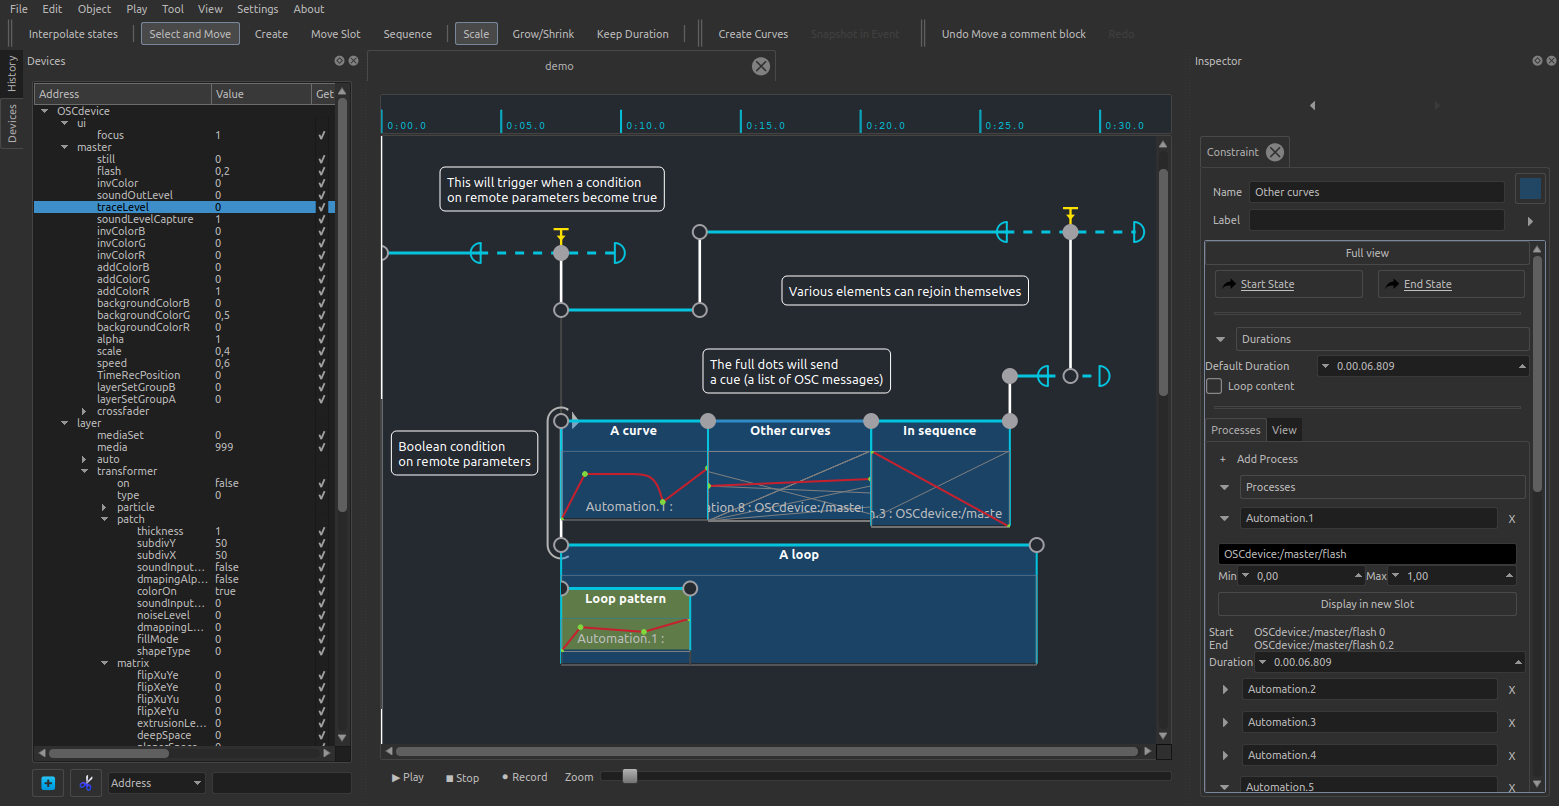
\includegraphics[width=\textwidth]{images/iscore.png}
		\end{figure}
	\end{frame}
	
	\begin{frame}
		\frametitle{Working with distributed software}
		\begin{figure}
			\centering
			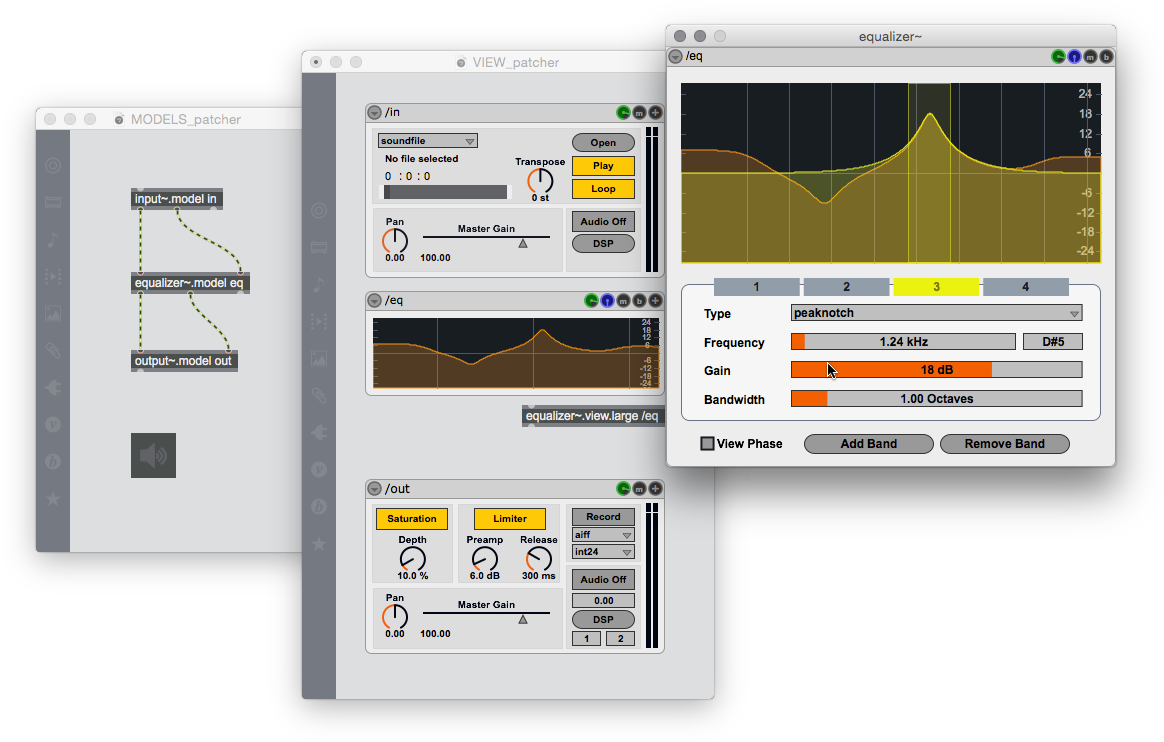
\includegraphics[width=\textwidth]{images/jamoma.jpg}
		\end{figure}
	\end{frame}
	
	\begin{frame}
		\frametitle{Conditions}
		\begin{figure}
			\centering\psscalebox{0.8}{
				%LaTeX with PSTricks extensions
%%Creator: inkscape 0.91
%%Please note this file requires PSTricks extensions
\psset{xunit=.5pt,yunit=.5pt,runit=.5pt}
\begin{pspicture}(744.09448819,1052.36220472)
{
\newrgbcolor{curcolor}{0.56862748 0.48627451 0.43529412}
\pscustom[linestyle=none,fillstyle=solid,fillcolor=curcolor]
{
\newpath
\moveto(413.9,957.89280472)
\lineto(415.9,957.89280472)
\lineto(415.9,589.89280472)
\lineto(413.9,589.89280472)
\closepath
}
}
{
\newrgbcolor{curcolor}{0.36470589 0.47843137 0.21568628}
\pscustom[linestyle=none,fillstyle=solid,fillcolor=curcolor,opacity=0]
{
\newpath
\moveto(421.4,969.39280472)
\lineto(421.6516,969.58579472)
\curveto(419.6656,970.73503172)(417.3596,971.39280472)(414.9,971.39280472)
\curveto(407.44416,971.39280472)(401.4,965.34864472)(401.4,957.89280472)
\lineto(401.4,865.89280472)
\curveto(401.4,858.43680472)(407.44416,852.39280472)(414.9,852.39280472)
\curveto(417.3599,852.39280472)(419.6662,853.05080472)(421.6524,854.19980472)
}
}
{
\newrgbcolor{curcolor}{0.43921569 0.85490197 0.21176471}
\pscustom[linewidth=2,linecolor=curcolor]
{
\newpath
\moveto(421.4,969.39280472)
\lineto(421.6516,969.58579472)
\curveto(419.6656,970.73503172)(417.3596,971.39280472)(414.9,971.39280472)
\curveto(407.44416,971.39280472)(401.4,965.34864472)(401.4,957.89280472)
\lineto(401.4,865.89280472)
\curveto(401.4,858.43680472)(407.44416,852.39280472)(414.9,852.39280472)
\curveto(417.3599,852.39280472)(419.6662,853.05080472)(421.6524,854.19980472)
}
}
{
\newrgbcolor{curcolor}{1 1 1}
\pscustom[linestyle=none,fillstyle=solid,fillcolor=curcolor]
{
\newpath
\moveto(426.4,966.39280472)
\lineto(426.4,950.39280472)
\lineto(433.4,957.39280472)
}
}
{
\newrgbcolor{curcolor}{1 1 1}
\pscustom[linewidth=1,linecolor=curcolor]
{
\newpath
\moveto(426.4,966.39280472)
\lineto(426.4,950.39280472)
\lineto(433.4,957.39280472)
}
}
{
\newrgbcolor{curcolor}{1 1 1}
\pscustom[linestyle=none,fillstyle=solid,fillcolor=curcolor]
{
\newpath
\moveto(413.60000005,957.89280472)
\lineto(416.19999995,957.89280472)
\lineto(416.19999995,865.89280472)
\lineto(413.60000005,865.89280472)
\closepath
}
}
{
\newrgbcolor{curcolor}{0.43921569 0.85490197 0.21176471}
\pscustom[linewidth=1,linecolor=curcolor]
{
\newpath
\moveto(413.60000005,957.89280472)
\lineto(416.19999995,957.89280472)
\lineto(416.19999995,865.89280472)
\lineto(413.60000005,865.89280472)
\closepath
}
}
{
\newrgbcolor{curcolor}{0.36470589 0.47843137 0.21568628}
\pscustom[linestyle=none,fillstyle=solid,fillcolor=curcolor,opacity=0]
{
\newpath
\moveto(421.4,749.39280472)
\lineto(421.6516,749.58579472)
\curveto(419.6656,750.73503172)(417.3596,751.39280472)(414.9,751.39280472)
\curveto(407.44416,751.39280472)(401.4,745.34864472)(401.4,737.89280472)
\lineto(401.4,589.89280472)
\curveto(401.4,582.43680472)(407.44416,576.39280472)(414.9,576.39280472)
\curveto(417.3599,576.39280472)(419.6662,577.05080472)(421.6524,578.19980472)
}
}
{
\newrgbcolor{curcolor}{0.85490197 0.37254903 0.21176471}
\pscustom[linewidth=2,linecolor=curcolor]
{
\newpath
\moveto(421.4,749.39280472)
\lineto(421.6516,749.58579472)
\curveto(419.6656,750.73503172)(417.3596,751.39280472)(414.9,751.39280472)
\curveto(407.44416,751.39280472)(401.4,745.34864472)(401.4,737.89280472)
\lineto(401.4,589.89280472)
\curveto(401.4,582.43680472)(407.44416,576.39280472)(414.9,576.39280472)
\curveto(417.3599,576.39280472)(419.6662,577.05080472)(421.6524,578.19980472)
}
}
{
\newrgbcolor{curcolor}{1 1 1}
\pscustom[linestyle=none,fillstyle=solid,fillcolor=curcolor]
{
\newpath
\moveto(426.4,746.39280472)
\lineto(426.4,730.39280472)
\lineto(433.4,737.39280472)
}
}
{
\newrgbcolor{curcolor}{1 1 1}
\pscustom[linewidth=1,linecolor=curcolor]
{
\newpath
\moveto(426.4,746.39280472)
\lineto(426.4,730.39280472)
\lineto(433.4,737.39280472)
}
}
{
\newrgbcolor{curcolor}{1 1 1}
\pscustom[linestyle=none,fillstyle=solid,fillcolor=curcolor]
{
\newpath
\moveto(413.60000005,737.89280472)
\lineto(416.19999995,737.89280472)
\lineto(416.19999995,589.89280472)
\lineto(413.60000005,589.89280472)
\closepath
}
}
{
\newrgbcolor{curcolor}{0.85490197 0.37254903 0.21176471}
\pscustom[linewidth=1,linecolor=curcolor]
{
\newpath
\moveto(413.60000005,737.89280472)
\lineto(416.19999995,737.89280472)
\lineto(416.19999995,589.89280472)
\lineto(413.60000005,589.89280472)
\closepath
}
}
{
\newrgbcolor{curcolor}{0.01176471 0.7647059 0.86666667}
\pscustom[linewidth=3,linecolor=curcolor]
{
\newpath
\moveto(34.615,957.89280472)
\lineto(414.9,957.89280472)
}
}
{
\newrgbcolor{curcolor}{0.01176471 0.7647059 0.86666667}
\pscustom[linewidth=3,linecolor=curcolor]
{
\newpath
\moveto(414.9,865.89280472)
\lineto(569.319,865.89280472)
}
}
{
\newrgbcolor{curcolor}{0.01176471 0.7647059 0.86666667}
\pscustom[linewidth=3,linecolor=curcolor]
{
\newpath
\moveto(414.9,737.89280472)
\lineto(668.424,737.89280472)
}
}
{
\newrgbcolor{curcolor}{0.01176471 0.7647059 0.86666667}
\pscustom[linewidth=3,linecolor=curcolor]
{
\newpath
\moveto(414.9,656.89280472)
\lineto(631.547,656.89280472)
}
}
{
\newrgbcolor{curcolor}{0.14509805 0.16078432 0.1882353}
\pscustom[linestyle=none,fillstyle=solid,fillcolor=curcolor]
{
\newpath
\moveto(41.615,957.89280472)
\curveto(41.615,954.02681148)(38.48099325,950.89280472)(34.615,950.89280472)
\curveto(30.74900675,950.89280472)(27.615,954.02681148)(27.615,957.89280472)
\curveto(27.615,961.75879797)(30.74900675,964.89280472)(34.615,964.89280472)
\curveto(38.48099325,964.89280472)(41.615,961.75879797)(41.615,957.89280472)
\closepath
}
}
{
\newrgbcolor{curcolor}{0.627451 0.627451 0.64313728}
\pscustom[linewidth=2,linecolor=curcolor]
{
\newpath
\moveto(41.615,957.89280472)
\curveto(41.615,954.02681148)(38.48099325,950.89280472)(34.615,950.89280472)
\curveto(30.74900675,950.89280472)(27.615,954.02681148)(27.615,957.89280472)
\curveto(27.615,961.75879797)(30.74900675,964.89280472)(34.615,964.89280472)
\curveto(38.48099325,964.89280472)(41.615,961.75879797)(41.615,957.89280472)
\closepath
}
}
{
\newrgbcolor{curcolor}{0.14509805 0.16078432 0.1882353}
\pscustom[linestyle=none,fillstyle=solid,fillcolor=curcolor]
{
\newpath
\moveto(421.9,957.89280472)
\curveto(421.9,954.02681148)(418.76599325,950.89280472)(414.9,950.89280472)
\curveto(411.03400675,950.89280472)(407.9,954.02681148)(407.9,957.89280472)
\curveto(407.9,961.75879797)(411.03400675,964.89280472)(414.9,964.89280472)
\curveto(418.76599325,964.89280472)(421.9,961.75879797)(421.9,957.89280472)
\closepath
}
}
{
\newrgbcolor{curcolor}{0.627451 0.627451 0.64313728}
\pscustom[linewidth=2,linecolor=curcolor]
{
\newpath
\moveto(421.9,957.89280472)
\curveto(421.9,954.02681148)(418.76599325,950.89280472)(414.9,950.89280472)
\curveto(411.03400675,950.89280472)(407.9,954.02681148)(407.9,957.89280472)
\curveto(407.9,961.75879797)(411.03400675,964.89280472)(414.9,964.89280472)
\curveto(418.76599325,964.89280472)(421.9,961.75879797)(421.9,957.89280472)
\closepath
}
}
{
\newrgbcolor{curcolor}{0.14509805 0.16078432 0.1882353}
\pscustom[linestyle=none,fillstyle=solid,fillcolor=curcolor]
{
\newpath
\moveto(421.9,865.89280472)
\curveto(421.9,862.02681148)(418.76599325,858.89280472)(414.9,858.89280472)
\curveto(411.03400675,858.89280472)(407.9,862.02681148)(407.9,865.89280472)
\curveto(407.9,869.75879797)(411.03400675,872.89280472)(414.9,872.89280472)
\curveto(418.76599325,872.89280472)(421.9,869.75879797)(421.9,865.89280472)
\closepath
}
}
{
\newrgbcolor{curcolor}{0.627451 0.627451 0.64313728}
\pscustom[linewidth=2,linecolor=curcolor]
{
\newpath
\moveto(421.9,865.89280472)
\curveto(421.9,862.02681148)(418.76599325,858.89280472)(414.9,858.89280472)
\curveto(411.03400675,858.89280472)(407.9,862.02681148)(407.9,865.89280472)
\curveto(407.9,869.75879797)(411.03400675,872.89280472)(414.9,872.89280472)
\curveto(418.76599325,872.89280472)(421.9,869.75879797)(421.9,865.89280472)
\closepath
}
}
{
\newrgbcolor{curcolor}{0.14509805 0.16078432 0.1882353}
\pscustom[linestyle=none,fillstyle=solid,fillcolor=curcolor]
{
\newpath
\moveto(576.318997,865.89280472)
\curveto(576.318997,862.02681148)(573.18499025,858.89280472)(569.318997,858.89280472)
\curveto(565.45300375,858.89280472)(562.318997,862.02681148)(562.318997,865.89280472)
\curveto(562.318997,869.75879797)(565.45300375,872.89280472)(569.318997,872.89280472)
\curveto(573.18499025,872.89280472)(576.318997,869.75879797)(576.318997,865.89280472)
\closepath
}
}
{
\newrgbcolor{curcolor}{0.627451 0.627451 0.64313728}
\pscustom[linewidth=2,linecolor=curcolor]
{
\newpath
\moveto(576.318997,865.89280472)
\curveto(576.318997,862.02681148)(573.18499025,858.89280472)(569.318997,858.89280472)
\curveto(565.45300375,858.89280472)(562.318997,862.02681148)(562.318997,865.89280472)
\curveto(562.318997,869.75879797)(565.45300375,872.89280472)(569.318997,872.89280472)
\curveto(573.18499025,872.89280472)(576.318997,869.75879797)(576.318997,865.89280472)
\closepath
}
}
{
\newrgbcolor{curcolor}{0.14509805 0.16078432 0.1882353}
\pscustom[linestyle=none,fillstyle=solid,fillcolor=curcolor]
{
\newpath
\moveto(421.9,737.89280472)
\curveto(421.9,734.02681148)(418.76599325,730.89280472)(414.9,730.89280472)
\curveto(411.03400675,730.89280472)(407.9,734.02681148)(407.9,737.89280472)
\curveto(407.9,741.75879797)(411.03400675,744.89280472)(414.9,744.89280472)
\curveto(418.76599325,744.89280472)(421.9,741.75879797)(421.9,737.89280472)
\closepath
}
}
{
\newrgbcolor{curcolor}{0.627451 0.627451 0.64313728}
\pscustom[linewidth=2,linecolor=curcolor]
{
\newpath
\moveto(421.9,737.89280472)
\curveto(421.9,734.02681148)(418.76599325,730.89280472)(414.9,730.89280472)
\curveto(411.03400675,730.89280472)(407.9,734.02681148)(407.9,737.89280472)
\curveto(407.9,741.75879797)(411.03400675,744.89280472)(414.9,744.89280472)
\curveto(418.76599325,744.89280472)(421.9,741.75879797)(421.9,737.89280472)
\closepath
}
}
{
\newrgbcolor{curcolor}{0.14509805 0.16078432 0.1882353}
\pscustom[linestyle=none,fillstyle=solid,fillcolor=curcolor]
{
\newpath
\moveto(675.423997,737.89280472)
\curveto(675.423997,734.02681148)(672.28999025,730.89280472)(668.423997,730.89280472)
\curveto(664.55800375,730.89280472)(661.423997,734.02681148)(661.423997,737.89280472)
\curveto(661.423997,741.75879797)(664.55800375,744.89280472)(668.423997,744.89280472)
\curveto(672.28999025,744.89280472)(675.423997,741.75879797)(675.423997,737.89280472)
\closepath
}
}
{
\newrgbcolor{curcolor}{0.627451 0.627451 0.64313728}
\pscustom[linewidth=2,linecolor=curcolor]
{
\newpath
\moveto(675.423997,737.89280472)
\curveto(675.423997,734.02681148)(672.28999025,730.89280472)(668.423997,730.89280472)
\curveto(664.55800375,730.89280472)(661.423997,734.02681148)(661.423997,737.89280472)
\curveto(661.423997,741.75879797)(664.55800375,744.89280472)(668.423997,744.89280472)
\curveto(672.28999025,744.89280472)(675.423997,741.75879797)(675.423997,737.89280472)
\closepath
}
}
{
\newrgbcolor{curcolor}{0.14509805 0.16078432 0.1882353}
\pscustom[linestyle=none,fillstyle=solid,fillcolor=curcolor]
{
\newpath
\moveto(421.9,656.89280472)
\curveto(421.9,653.02681148)(418.76599325,649.89280472)(414.9,649.89280472)
\curveto(411.03400675,649.89280472)(407.9,653.02681148)(407.9,656.89280472)
\curveto(407.9,660.75879797)(411.03400675,663.89280472)(414.9,663.89280472)
\curveto(418.76599325,663.89280472)(421.9,660.75879797)(421.9,656.89280472)
\closepath
}
}
{
\newrgbcolor{curcolor}{0.627451 0.627451 0.64313728}
\pscustom[linewidth=2,linecolor=curcolor]
{
\newpath
\moveto(421.9,656.89280472)
\curveto(421.9,653.02681148)(418.76599325,649.89280472)(414.9,649.89280472)
\curveto(411.03400675,649.89280472)(407.9,653.02681148)(407.9,656.89280472)
\curveto(407.9,660.75879797)(411.03400675,663.89280472)(414.9,663.89280472)
\curveto(418.76599325,663.89280472)(421.9,660.75879797)(421.9,656.89280472)
\closepath
}
}
{
\newrgbcolor{curcolor}{0.14509805 0.16078432 0.1882353}
\pscustom[linestyle=none,fillstyle=solid,fillcolor=curcolor]
{
\newpath
\moveto(638.547997,656.89280472)
\curveto(638.547997,653.02681148)(635.41399025,649.89280472)(631.547997,649.89280472)
\curveto(627.68200375,649.89280472)(624.547997,653.02681148)(624.547997,656.89280472)
\curveto(624.547997,660.75879797)(627.68200375,663.89280472)(631.547997,663.89280472)
\curveto(635.41399025,663.89280472)(638.547997,660.75879797)(638.547997,656.89280472)
\closepath
}
}
{
\newrgbcolor{curcolor}{0.627451 0.627451 0.64313728}
\pscustom[linewidth=2,linecolor=curcolor]
{
\newpath
\moveto(638.547997,656.89280472)
\curveto(638.547997,653.02681148)(635.41399025,649.89280472)(631.547997,649.89280472)
\curveto(627.68200375,649.89280472)(624.547997,653.02681148)(624.547997,656.89280472)
\curveto(624.547997,660.75879797)(627.68200375,663.89280472)(631.547997,663.89280472)
\curveto(635.41399025,663.89280472)(638.547997,660.75879797)(638.547997,656.89280472)
\closepath
}
}
{
\newrgbcolor{curcolor}{0.14509805 0.16078432 0.1882353}
\pscustom[linestyle=none,fillstyle=solid,fillcolor=curcolor]
{
\newpath
\moveto(421.9,589.89280472)
\curveto(421.9,586.02681148)(418.76599325,582.89280472)(414.9,582.89280472)
\curveto(411.03400675,582.89280472)(407.9,586.02681148)(407.9,589.89280472)
\curveto(407.9,593.75879797)(411.03400675,596.89280472)(414.9,596.89280472)
\curveto(418.76599325,596.89280472)(421.9,593.75879797)(421.9,589.89280472)
\closepath
}
}
{
\newrgbcolor{curcolor}{0.627451 0.627451 0.64313728}
\pscustom[linewidth=2,linecolor=curcolor]
{
\newpath
\moveto(421.9,589.89280472)
\curveto(421.9,586.02681148)(418.76599325,582.89280472)(414.9,582.89280472)
\curveto(411.03400675,582.89280472)(407.9,586.02681148)(407.9,589.89280472)
\curveto(407.9,593.75879797)(411.03400675,596.89280472)(414.9,596.89280472)
\curveto(418.76599325,596.89280472)(421.9,593.75879797)(421.9,589.89280472)
\closepath
}
}
{
\newrgbcolor{curcolor}{0 0 0}
\pscustom[linestyle=none,fillstyle=solid,fillcolor=curcolor]
{
\newpath
\moveto(186.5709901,905.5161557)
\lineto(186.5709901,913.1061557)
\curveto(186.5709901,916.2261557)(184.5909901,918.2061557)(180.6609901,918.2061557)
\curveto(179.1009901,918.2061557)(177.4209901,917.9061557)(175.4709901,917.2161557)
\lineto(176.1609901,915.2961557)
\curveto(177.7809901,915.8661557)(179.2209901,916.1061557)(180.2709901,916.1061557)
\curveto(182.6109901,916.1061557)(184.0209901,915.2661557)(184.0209901,912.9561557)
\lineto(184.0209901,911.6661557)
\lineto(181.6809901,911.6661557)
\curveto(176.9109901,911.6661557)(174.3009901,909.8361557)(174.3009901,906.5961557)
\curveto(174.3009901,903.6561557)(176.2209901,901.7361557)(179.4009901,901.7361557)
\curveto(181.4409901,901.7361557)(183.2109901,902.4861557)(184.3509901,903.9561557)
\curveto(184.7709901,902.5161557)(185.8809901,901.8861557)(187.2309901,901.7061557)
\lineto(187.8609901,903.5061557)
\curveto(186.9609901,903.7761557)(186.5709901,904.2561557)(186.5709901,905.5161557)
\closepath
\moveto(180.0309901,903.6261557)
\curveto(177.9609901,903.6261557)(177.0009901,904.6461557)(177.0009901,906.6261557)
\curveto(177.0009901,908.6661557)(178.2609901,909.9261557)(181.7409901,909.9261557)
\lineto(184.0209901,909.9261557)
\lineto(184.0209901,905.8761557)
\curveto(183.0909901,904.4661557)(181.5909901,903.6261557)(180.0309901,903.6261557)
\closepath
}
}
{
\newrgbcolor{curcolor}{0 0 0}
\pscustom[linestyle=none,fillstyle=solid,fillcolor=curcolor]
{
\newpath
\moveto(196.78927135,914.9961557)
\curveto(196.78927135,913.6461557)(197.80927135,912.5361557)(199.18927135,912.5361557)
\curveto(200.59927135,912.5361557)(201.61927135,913.6461557)(201.61927135,914.9961557)
\curveto(201.61927135,916.3161557)(200.59927135,917.3961557)(199.18927135,917.3961557)
\curveto(197.80927135,917.3961557)(196.78927135,916.3161557)(196.78927135,914.9961557)
\closepath
\moveto(196.78927135,904.1661557)
\curveto(196.78927135,902.7861557)(197.80927135,901.7361557)(199.18927135,901.7361557)
\curveto(200.59927135,901.7361557)(201.61927135,902.7861557)(201.61927135,904.1661557)
\curveto(201.61927135,905.4861557)(200.59927135,906.5961557)(199.18927135,906.5961557)
\curveto(197.80927135,906.5961557)(196.78927135,905.4861557)(196.78927135,904.1661557)
\closepath
}
}
{
\newrgbcolor{curcolor}{0 0 0}
\pscustom[linestyle=none,fillstyle=solid,fillcolor=curcolor]
{
\newpath
\moveto(211.8375526,898.9761557)
\lineto(224.6175526,925.3761557)
\lineto(222.6075526,926.3361557)
\lineto(209.7975526,899.8761557)
\lineto(211.8375526,898.9761557)
\closepath
}
}
{
\newrgbcolor{curcolor}{0 0 0}
\pscustom[linestyle=none,fillstyle=solid,fillcolor=curcolor]
{
\newpath
\moveto(238.52583385,924.5361557)
\curveto(235.25583385,924.5361557)(232.76583385,922.7061557)(232.76583385,919.7961557)
\lineto(232.76583385,916.6461557)
\lineto(229.01583385,916.6461557)
\lineto(229.01583385,914.6361557)
\lineto(232.76583385,914.6361557)
\lineto(232.76583385,902.0661557)
\lineto(235.31583385,902.0661557)
\lineto(235.31583385,914.6361557)
\lineto(240.38583385,914.6361557)
\lineto(240.65583385,916.6461557)
\lineto(235.31583385,916.6461557)
\lineto(235.31583385,919.8561557)
\curveto(235.31583385,921.5961557)(236.42583385,922.4661557)(238.61583385,922.4661557)
\curveto(239.81583385,922.4661557)(240.98583385,922.2561557)(242.00583385,921.8061557)
\lineto(242.81583385,923.6961557)
\curveto(241.58583385,924.2061557)(240.23583385,924.5361557)(238.52583385,924.5361557)
\closepath
}
}
{
\newrgbcolor{curcolor}{0 0 0}
\pscustom[linestyle=none,fillstyle=solid,fillcolor=curcolor]
{
\newpath
\moveto(253.2141151,918.2061557)
\curveto(248.7741151,918.2061557)(246.3741151,914.8161557)(246.3741151,909.9561557)
\curveto(246.3741151,904.9761557)(248.7441151,901.7361557)(253.1841151,901.7361557)
\curveto(257.5941151,901.7361557)(259.9941151,905.1261557)(259.9941151,909.9861557)
\curveto(259.9941151,914.9661557)(257.6541151,918.2061557)(253.2141151,918.2061557)
\closepath
\moveto(253.2141151,916.1361557)
\curveto(255.9141151,916.1361557)(257.2641151,914.1561557)(257.2641151,909.9861557)
\curveto(257.2641151,905.7561557)(255.9141151,903.8061557)(253.1841151,903.8061557)
\curveto(250.4541151,903.8061557)(249.1041151,905.7561557)(249.1041151,909.9561557)
\curveto(249.1041151,914.1561557)(250.4841151,916.1361557)(253.2141151,916.1361557)
\closepath
}
}
{
\newrgbcolor{curcolor}{0 0 0}
\pscustom[linestyle=none,fillstyle=solid,fillcolor=curcolor]
{
\newpath
\moveto(271.20239635,918.2061557)
\curveto(266.76239635,918.2061557)(264.36239635,914.8161557)(264.36239635,909.9561557)
\curveto(264.36239635,904.9761557)(266.73239635,901.7361557)(271.17239635,901.7361557)
\curveto(275.58239635,901.7361557)(277.98239635,905.1261557)(277.98239635,909.9861557)
\curveto(277.98239635,914.9661557)(275.64239635,918.2061557)(271.20239635,918.2061557)
\closepath
\moveto(271.20239635,916.1361557)
\curveto(273.90239635,916.1361557)(275.25239635,914.1561557)(275.25239635,909.9861557)
\curveto(275.25239635,905.7561557)(273.90239635,903.8061557)(271.17239635,903.8061557)
\curveto(268.44239635,903.8061557)(267.09239635,905.7561557)(267.09239635,909.9561557)
\curveto(267.09239635,914.1561557)(268.47239635,916.1361557)(271.20239635,916.1361557)
\closepath
}
}
{
\newrgbcolor{curcolor}{0 0 0}
\pscustom[linestyle=none,fillstyle=solid,fillcolor=curcolor]
{
\newpath
\moveto(312.30895885,919.8861557)
\lineto(300.78895885,912.7761557)
\lineto(300.78895885,910.1661557)
\lineto(312.18895885,903.0561557)
\lineto(313.53895885,904.8861557)
\lineto(302.94895885,911.4561557)
\lineto(313.53895885,917.9661557)
\lineto(312.30895885,919.8861557)
\closepath
}
}
{
\newrgbcolor{curcolor}{0 0 0}
\pscustom[linestyle=none,fillstyle=solid,fillcolor=curcolor]
{
\newpath
\moveto(342.19552135,923.0661557)
\curveto(339.40552135,923.0661557)(337.51552135,922.0761557)(335.89552135,920.0961557)
\lineto(337.63552135,918.7461557)
\curveto(338.95552135,920.2761557)(340.06552135,920.9361557)(342.07552135,920.9361557)
\curveto(344.38552135,920.9361557)(345.79552135,919.5261557)(345.79552135,917.2161557)
\curveto(345.79552135,913.8561557)(344.11552135,911.5761557)(336.31552135,904.1061557)
\lineto(336.31552135,902.0661557)
\lineto(348.61552135,902.0661557)
\lineto(348.91552135,904.2261557)
\lineto(339.19552135,904.2261557)
\curveto(346.00552135,910.4361557)(348.43552135,913.4961557)(348.43552135,917.3061557)
\curveto(348.43552135,920.5761557)(346.09552135,923.0661557)(342.19552135,923.0661557)
\closepath
}
}
{
\newrgbcolor{curcolor}{0 0 0}
\pscustom[linestyle=none,fillstyle=solid,fillcolor=curcolor]
{
\newpath
\moveto(358.4438026,904.3761557)
\curveto(358.4438026,902.8761557)(359.5838026,901.7361557)(361.0838026,901.7361557)
\curveto(362.6138026,901.7361557)(363.7238026,902.8761557)(363.7238026,904.3761557)
\curveto(363.7238026,905.8461557)(362.6138026,907.0161557)(361.0838026,907.0161557)
\curveto(359.5838026,907.0161557)(358.4438026,905.8461557)(358.4438026,904.3761557)
\closepath
}
}
{
\newrgbcolor{curcolor}{0 0 0}
\pscustom[linestyle=none,fillstyle=solid,fillcolor=curcolor]
{
\newpath
\moveto(378.17208385,923.0661557)
\curveto(376.04208385,923.0661557)(374.06208385,922.3461557)(372.29208385,920.6661557)
\lineto(373.67208385,919.1361557)
\curveto(375.05208385,920.3961557)(376.28208385,921.0261557)(378.05208385,921.0261557)
\curveto(380.24208385,921.0261557)(381.95208385,919.7961557)(381.95208385,917.5461557)
\curveto(381.95208385,915.0561557)(380.03208385,913.9461557)(378.05208385,913.9461557)
\lineto(376.82208385,913.9461557)
\lineto(376.52208385,911.9361557)
\lineto(378.23208385,911.9361557)
\curveto(380.69208385,911.9361557)(382.52208385,910.9761557)(382.52208385,908.0061557)
\curveto(382.52208385,905.4261557)(380.81208385,903.8061557)(377.93208385,903.8061557)
\curveto(376.25208385,903.8061557)(374.51208385,904.4661557)(373.34208385,905.8461557)
\lineto(371.66208385,904.4661557)
\curveto(373.22208385,902.5761557)(375.68208385,901.7361557)(377.99208385,901.7361557)
\curveto(382.28208385,901.7361557)(385.16208385,904.4361557)(385.16208385,908.0061557)
\curveto(385.16208385,911.2161557)(382.88208385,912.8961557)(380.48208385,913.0761557)
\curveto(382.64208385,913.4961557)(384.50208385,915.3861557)(384.50208385,917.8761557)
\curveto(384.50208385,920.6961557)(382.07208385,923.0661557)(378.17208385,923.0661557)
\closepath
}
}
{
\newrgbcolor{curcolor}{0 0 0}
\pscustom[linestyle=none,fillstyle=solid,fillcolor=curcolor]
{
\newpath
\moveto(143.13446666,661.05924652)
\lineto(143.13446666,668.64924652)
\curveto(143.13446666,671.76924652)(141.15446666,673.74924652)(137.22446666,673.74924652)
\curveto(135.66446666,673.74924652)(133.98446666,673.44924652)(132.03446666,672.75924652)
\lineto(132.72446666,670.83924652)
\curveto(134.34446666,671.40924652)(135.78446666,671.64924652)(136.83446666,671.64924652)
\curveto(139.17446666,671.64924652)(140.58446666,670.80924652)(140.58446666,668.49924652)
\lineto(140.58446666,667.20924652)
\lineto(138.24446666,667.20924652)
\curveto(133.47446666,667.20924652)(130.86446666,665.37924652)(130.86446666,662.13924652)
\curveto(130.86446666,659.19924652)(132.78446666,657.27924652)(135.96446666,657.27924652)
\curveto(138.00446666,657.27924652)(139.77446666,658.02924652)(140.91446666,659.49924652)
\curveto(141.33446666,658.05924652)(142.44446666,657.42924652)(143.79446666,657.24924652)
\lineto(144.42446666,659.04924652)
\curveto(143.52446666,659.31924652)(143.13446666,659.79924652)(143.13446666,661.05924652)
\closepath
\moveto(136.59446666,659.16924652)
\curveto(134.52446666,659.16924652)(133.56446666,660.18924652)(133.56446666,662.16924652)
\curveto(133.56446666,664.20924652)(134.82446666,665.46924652)(138.30446666,665.46924652)
\lineto(140.58446666,665.46924652)
\lineto(140.58446666,661.41924652)
\curveto(139.65446666,660.00924652)(138.15446666,659.16924652)(136.59446666,659.16924652)
\closepath
}
}
{
\newrgbcolor{curcolor}{0 0 0}
\pscustom[linestyle=none,fillstyle=solid,fillcolor=curcolor]
{
\newpath
\moveto(153.35274791,670.53924652)
\curveto(153.35274791,669.18924652)(154.37274791,668.07924652)(155.75274791,668.07924652)
\curveto(157.16274791,668.07924652)(158.18274791,669.18924652)(158.18274791,670.53924652)
\curveto(158.18274791,671.85924652)(157.16274791,672.93924652)(155.75274791,672.93924652)
\curveto(154.37274791,672.93924652)(153.35274791,671.85924652)(153.35274791,670.53924652)
\closepath
\moveto(153.35274791,659.70924652)
\curveto(153.35274791,658.32924652)(154.37274791,657.27924652)(155.75274791,657.27924652)
\curveto(157.16274791,657.27924652)(158.18274791,658.32924652)(158.18274791,659.70924652)
\curveto(158.18274791,661.02924652)(157.16274791,662.13924652)(155.75274791,662.13924652)
\curveto(154.37274791,662.13924652)(153.35274791,661.02924652)(153.35274791,659.70924652)
\closepath
}
}
{
\newrgbcolor{curcolor}{0 0 0}
\pscustom[linestyle=none,fillstyle=solid,fillcolor=curcolor]
{
\newpath
\moveto(168.40102916,654.51924652)
\lineto(181.18102916,680.91924652)
\lineto(179.17102916,681.87924652)
\lineto(166.36102916,655.41924652)
\lineto(168.40102916,654.51924652)
\closepath
}
}
{
\newrgbcolor{curcolor}{0 0 0}
\pscustom[linestyle=none,fillstyle=solid,fillcolor=curcolor]
{
\newpath
\moveto(188.27931041,671.34924652)
\lineto(188.27931041,680.07924652)
\lineto(185.75931041,679.77924652)
\lineto(185.75931041,657.60924652)
\lineto(187.97931041,657.60924652)
\lineto(188.15931041,659.25924652)
\curveto(189.23931041,657.87924652)(190.64931041,657.27924652)(192.44931041,657.27924652)
\curveto(196.52931041,657.27924652)(198.71931041,660.72924652)(198.71931041,665.52924652)
\curveto(198.71931041,670.47924652)(197.00931041,673.74924652)(192.80931041,673.74924652)
\curveto(190.97931041,673.74924652)(189.44931041,672.87924652)(188.27931041,671.34924652)
\closepath
\moveto(191.87931041,659.31924652)
\curveto(190.40931041,659.31924652)(189.11931041,660.06924652)(188.27931041,661.35924652)
\lineto(188.27931041,669.18924652)
\curveto(189.14931041,670.44924652)(190.49931041,671.70924652)(192.23931041,671.70924652)
\curveto(194.69931041,671.70924652)(195.98931041,669.63924652)(195.98931041,665.52924652)
\curveto(195.98931041,661.32924652)(194.48931041,659.31924652)(191.87931041,659.31924652)
\closepath
}
}
{
\newrgbcolor{curcolor}{0 0 0}
\pscustom[linestyle=none,fillstyle=solid,fillcolor=curcolor]
{
\newpath
\moveto(215.08759166,661.05924652)
\lineto(215.08759166,668.64924652)
\curveto(215.08759166,671.76924652)(213.10759166,673.74924652)(209.17759166,673.74924652)
\curveto(207.61759166,673.74924652)(205.93759166,673.44924652)(203.98759166,672.75924652)
\lineto(204.67759166,670.83924652)
\curveto(206.29759166,671.40924652)(207.73759166,671.64924652)(208.78759166,671.64924652)
\curveto(211.12759166,671.64924652)(212.53759166,670.80924652)(212.53759166,668.49924652)
\lineto(212.53759166,667.20924652)
\lineto(210.19759166,667.20924652)
\curveto(205.42759166,667.20924652)(202.81759166,665.37924652)(202.81759166,662.13924652)
\curveto(202.81759166,659.19924652)(204.73759166,657.27924652)(207.91759166,657.27924652)
\curveto(209.95759166,657.27924652)(211.72759166,658.02924652)(212.86759166,659.49924652)
\curveto(213.28759166,658.05924652)(214.39759166,657.42924652)(215.74759166,657.24924652)
\lineto(216.37759166,659.04924652)
\curveto(215.47759166,659.31924652)(215.08759166,659.79924652)(215.08759166,661.05924652)
\closepath
\moveto(208.54759166,659.16924652)
\curveto(206.47759166,659.16924652)(205.51759166,660.18924652)(205.51759166,662.16924652)
\curveto(205.51759166,664.20924652)(206.77759166,665.46924652)(210.25759166,665.46924652)
\lineto(212.53759166,665.46924652)
\lineto(212.53759166,661.41924652)
\curveto(211.60759166,660.00924652)(210.10759166,659.16924652)(208.54759166,659.16924652)
\closepath
}
}
{
\newrgbcolor{curcolor}{0 0 0}
\pscustom[linestyle=none,fillstyle=solid,fillcolor=curcolor]
{
\newpath
\moveto(232.41587291,673.74924652)
\curveto(229.56587291,673.74924652)(227.94587291,672.24924652)(226.74587291,669.66924652)
\lineto(226.26587291,673.41924652)
\lineto(221.88587291,673.41924652)
\lineto(221.88587291,671.46924652)
\lineto(224.37587291,671.46924652)
\lineto(224.37587291,659.55924652)
\lineto(221.88587291,659.55924652)
\lineto(221.88587291,657.60924652)
\lineto(230.10587291,657.60924652)
\lineto(230.10587291,659.55924652)
\lineto(226.89587291,659.55924652)
\lineto(226.89587291,666.21924652)
\curveto(227.91587291,669.69924652)(229.65587291,671.43924652)(232.08587291,671.43924652)
\lineto(232.23587291,671.43924652)
\lineto(232.23587291,668.04924652)
\lineto(234.27587291,668.04924652)
\lineto(234.63587291,673.41924652)
\curveto(233.94587291,673.59924652)(233.28587291,673.74924652)(232.41587291,673.74924652)
\closepath
}
}
{
\newrgbcolor{curcolor}{0 0 0}
\pscustom[linestyle=none,fillstyle=solid,fillcolor=curcolor]
{
\newpath
\moveto(287.52071666,668.70924652)
\lineto(287.52071666,670.86924652)
\lineto(276.24071666,670.86924652)
\lineto(279.45071666,676.26924652)
\lineto(277.50071666,677.25924652)
\lineto(273.69071666,670.86924652)
\lineto(257.88071666,670.86924652)
\lineto(257.88071666,668.70924652)
\lineto(272.37071666,668.70924652)
\lineto(270.27071666,665.16924652)
\lineto(257.88071666,665.16924652)
\lineto(257.88071666,663.00924652)
\lineto(268.98071666,663.00924652)
\lineto(265.95071666,657.96924652)
\lineto(267.96071666,656.94924652)
\lineto(271.56071666,663.00924652)
\lineto(287.52071666,663.00924652)
\lineto(287.52071666,665.16924652)
\lineto(272.85071666,665.16924652)
\lineto(274.95071666,668.70924652)
\lineto(287.52071666,668.70924652)
\closepath
}
}
{
\newrgbcolor{curcolor}{0 0 0}
\pscustom[linestyle=none,fillstyle=solid,fillcolor=curcolor]
{
\newpath
\moveto(314.04727916,671.97924652)
\lineto(316.26727916,671.97924652)
\lineto(316.74727916,679.77924652)
\lineto(313.59727916,679.77924652)
\lineto(314.04727916,671.97924652)
\closepath
\moveto(319.08727916,671.97924652)
\lineto(321.30727916,671.97924652)
\lineto(321.75727916,679.77924652)
\lineto(318.60727916,679.77924652)
\lineto(319.08727916,671.97924652)
\closepath
}
}
{
\newrgbcolor{curcolor}{0 0 0}
\pscustom[linestyle=none,fillstyle=solid,fillcolor=curcolor]
{
\newpath
\moveto(332.18556041,671.34924652)
\lineto(332.18556041,680.07924652)
\lineto(329.66556041,679.77924652)
\lineto(329.66556041,657.60924652)
\lineto(331.88556041,657.60924652)
\lineto(332.06556041,659.25924652)
\curveto(333.14556041,657.87924652)(334.55556041,657.27924652)(336.35556041,657.27924652)
\curveto(340.43556041,657.27924652)(342.62556041,660.72924652)(342.62556041,665.52924652)
\curveto(342.62556041,670.47924652)(340.91556041,673.74924652)(336.71556041,673.74924652)
\curveto(334.88556041,673.74924652)(333.35556041,672.87924652)(332.18556041,671.34924652)
\closepath
\moveto(335.78556041,659.31924652)
\curveto(334.31556041,659.31924652)(333.02556041,660.06924652)(332.18556041,661.35924652)
\lineto(332.18556041,669.18924652)
\curveto(333.05556041,670.44924652)(334.40556041,671.70924652)(336.14556041,671.70924652)
\curveto(338.60556041,671.70924652)(339.89556041,669.63924652)(339.89556041,665.52924652)
\curveto(339.89556041,661.32924652)(338.39556041,659.31924652)(335.78556041,659.31924652)
\closepath
}
}
{
\newrgbcolor{curcolor}{0 0 0}
\pscustom[linestyle=none,fillstyle=solid,fillcolor=curcolor]
{
\newpath
\moveto(353.68384166,673.74924652)
\curveto(349.24384166,673.74924652)(346.84384166,670.35924652)(346.84384166,665.49924652)
\curveto(346.84384166,660.51924652)(349.21384166,657.27924652)(353.65384166,657.27924652)
\curveto(358.06384166,657.27924652)(360.46384166,660.66924652)(360.46384166,665.52924652)
\curveto(360.46384166,670.50924652)(358.12384166,673.74924652)(353.68384166,673.74924652)
\closepath
\moveto(353.68384166,671.67924652)
\curveto(356.38384166,671.67924652)(357.73384166,669.69924652)(357.73384166,665.52924652)
\curveto(357.73384166,661.29924652)(356.38384166,659.34924652)(353.65384166,659.34924652)
\curveto(350.92384166,659.34924652)(349.57384166,661.29924652)(349.57384166,665.49924652)
\curveto(349.57384166,669.69924652)(350.95384166,671.67924652)(353.68384166,671.67924652)
\closepath
}
}
{
\newrgbcolor{curcolor}{0 0 0}
\pscustom[linestyle=none,fillstyle=solid,fillcolor=curcolor]
{
\newpath
\moveto(371.67212291,673.74924652)
\curveto(367.23212291,673.74924652)(364.83212291,670.35924652)(364.83212291,665.49924652)
\curveto(364.83212291,660.51924652)(367.20212291,657.27924652)(371.64212291,657.27924652)
\curveto(376.05212291,657.27924652)(378.45212291,660.66924652)(378.45212291,665.52924652)
\curveto(378.45212291,670.50924652)(376.11212291,673.74924652)(371.67212291,673.74924652)
\closepath
\moveto(371.67212291,671.67924652)
\curveto(374.37212291,671.67924652)(375.72212291,669.69924652)(375.72212291,665.52924652)
\curveto(375.72212291,661.29924652)(374.37212291,659.34924652)(371.64212291,659.34924652)
\curveto(368.91212291,659.34924652)(367.56212291,661.29924652)(367.56212291,665.49924652)
\curveto(367.56212291,669.69924652)(368.94212291,671.67924652)(371.67212291,671.67924652)
\closepath
}
}
{
\newrgbcolor{curcolor}{0 0 0}
\pscustom[linestyle=none,fillstyle=solid,fillcolor=curcolor]
{
\newpath
\moveto(386.00040416,671.97924652)
\lineto(388.22040416,671.97924652)
\lineto(388.70040416,679.77924652)
\lineto(385.55040416,679.77924652)
\lineto(386.00040416,671.97924652)
\closepath
\moveto(391.04040416,671.97924652)
\lineto(393.26040416,671.97924652)
\lineto(393.71040416,679.77924652)
\lineto(390.56040416,679.77924652)
\lineto(391.04040416,671.97924652)
\closepath
}
}
{
\newrgbcolor{curcolor}{0 0 0}
\pscustom[linewidth=4,linecolor=curcolor]
{
\newpath
\moveto(298.50008,1008.13220472)
\curveto(325.64601,1000.55460472)(389.77702,1018.31510472)(412.14224,980.85810472)
}
}
{
\newrgbcolor{curcolor}{0 0 0}
\pscustom[linestyle=none,fillstyle=solid,fillcolor=curcolor]
{
\newpath
\moveto(409.68148269,984.97935131)
\lineto(404.19647944,986.36309238)
\lineto(414.80806042,976.39342092)
\lineto(411.06522375,990.46435457)
\lineto(409.68148269,984.97935131)
\closepath
}
}
{
\newrgbcolor{curcolor}{0 0 0}
\pscustom[linewidth=1,linecolor=curcolor]
{
\newpath
\moveto(409.68148269,984.97935131)
\lineto(404.19647944,986.36309238)
\lineto(414.80806042,976.39342092)
\lineto(411.06522375,990.46435457)
\lineto(409.68148269,984.97935131)
\closepath
}
}
{
\newrgbcolor{curcolor}{0 0 0}
\pscustom[linestyle=none,fillstyle=solid,fillcolor=curcolor]
{
\newpath
\moveto(84.39559947,1040.92414398)
\lineto(73.20559947,1040.92414398)
\lineto(73.20559947,1020.25414398)
\lineto(84.63559947,1020.25414398)
\lineto(84.63559947,1022.53414398)
\lineto(76.05559947,1022.53414398)
\lineto(76.05559947,1029.61414398)
\lineto(83.01559947,1029.61414398)
\lineto(83.01559947,1031.89414398)
\lineto(76.05559947,1031.89414398)
\lineto(76.05559947,1038.64414398)
\lineto(84.06559947,1038.64414398)
\lineto(84.39559947,1040.92414398)
\closepath
}
}
{
\newrgbcolor{curcolor}{0 0 0}
\pscustom[linestyle=none,fillstyle=solid,fillcolor=curcolor]
{
\newpath
\moveto(100.72028697,1036.06414398)
\lineto(97.81028697,1036.06414398)
\lineto(93.70028697,1022.71414398)
\lineto(89.56028697,1036.06414398)
\lineto(86.56028697,1036.06414398)
\lineto(92.02028697,1020.25414398)
\lineto(95.35028697,1020.25414398)
\lineto(100.72028697,1036.06414398)
\closepath
}
}
{
\newrgbcolor{curcolor}{0 0 0}
\pscustom[linestyle=none,fillstyle=solid,fillcolor=curcolor]
{
\newpath
\moveto(114.52591197,1023.94414398)
\lineto(114.52591197,1031.17414398)
\curveto(114.52591197,1034.47414398)(112.78591197,1036.42414398)(108.97591197,1036.42414398)
\curveto(107.20591197,1036.42414398)(105.46591197,1036.06414398)(103.51591197,1035.34414398)
\lineto(104.20591197,1033.33414398)
\curveto(105.82591197,1033.87414398)(107.29591197,1034.17414398)(108.46591197,1034.17414398)
\curveto(110.65591197,1034.17414398)(111.76591197,1033.33414398)(111.76591197,1031.05414398)
\lineto(111.76591197,1029.88414398)
\lineto(109.33591197,1029.88414398)
\curveto(104.92591197,1029.88414398)(102.37591197,1028.05414398)(102.37591197,1024.66414398)
\curveto(102.37591197,1021.84414398)(104.26591197,1019.89414398)(107.41591197,1019.89414398)
\curveto(109.33591197,1019.89414398)(111.01591197,1020.61414398)(112.12591197,1022.26414398)
\curveto(112.60591197,1020.70414398)(113.62591197,1020.07414398)(115.21591197,1019.89414398)
\lineto(115.84591197,1021.81414398)
\curveto(115.03591197,1022.11414398)(114.52591197,1022.56414398)(114.52591197,1023.94414398)
\closepath
\moveto(108.04591197,1021.96414398)
\curveto(106.24591197,1021.96414398)(105.31591197,1022.95414398)(105.31591197,1024.81414398)
\curveto(105.31591197,1026.97414398)(106.78591197,1028.05414398)(109.69591197,1028.05414398)
\lineto(111.76591197,1028.05414398)
\lineto(111.76591197,1024.42414398)
\curveto(110.86591197,1022.77414398)(109.66591197,1021.96414398)(108.04591197,1021.96414398)
\closepath
}
}
{
\newrgbcolor{curcolor}{0 0 0}
\pscustom[linestyle=none,fillstyle=solid,fillcolor=curcolor]
{
\newpath
\moveto(123.37356822,1019.89414398)
\curveto(124.18356822,1019.89414398)(124.96356822,1020.10414398)(125.56356822,1020.43414398)
\lineto(124.84356822,1022.35414398)
\curveto(124.54356822,1022.23414398)(124.21356822,1022.17414398)(123.82356822,1022.17414398)
\curveto(123.10356822,1022.17414398)(122.83356822,1022.59414398)(122.83356822,1023.43414398)
\lineto(122.83356822,1042.75414398)
\lineto(120.07356822,1042.42414398)
\lineto(120.07356822,1023.37414398)
\curveto(120.07356822,1021.12414398)(121.36356822,1019.89414398)(123.37356822,1019.89414398)
\closepath
}
}
{
\newrgbcolor{curcolor}{0 0 0}
\pscustom[linestyle=none,fillstyle=solid,fillcolor=curcolor]
{
\newpath
\moveto(140.77263072,1036.06414398)
\lineto(138.01263072,1036.06414398)
\lineto(138.01263072,1024.78414398)
\curveto(137.05263072,1023.19414398)(135.76263072,1022.05414398)(134.05263072,1022.05414398)
\curveto(132.34263072,1022.05414398)(131.62263072,1022.86414398)(131.62263072,1025.02414398)
\lineto(131.62263072,1036.06414398)
\lineto(128.86263072,1036.06414398)
\lineto(128.86263072,1024.72414398)
\curveto(128.86263072,1021.63414398)(130.51263072,1019.89414398)(133.27263072,1019.89414398)
\curveto(135.52263072,1019.89414398)(136.99263072,1020.79414398)(138.19263072,1022.71414398)
\lineto(138.40263072,1020.25414398)
\lineto(140.77263072,1020.25414398)
\lineto(140.77263072,1036.06414398)
\closepath
}
}
{
\newrgbcolor{curcolor}{0 0 0}
\pscustom[linestyle=none,fillstyle=solid,fillcolor=curcolor]
{
\newpath
\moveto(157.12356822,1023.94414398)
\lineto(157.12356822,1031.17414398)
\curveto(157.12356822,1034.47414398)(155.38356822,1036.42414398)(151.57356822,1036.42414398)
\curveto(149.80356822,1036.42414398)(148.06356822,1036.06414398)(146.11356822,1035.34414398)
\lineto(146.80356822,1033.33414398)
\curveto(148.42356822,1033.87414398)(149.89356822,1034.17414398)(151.06356822,1034.17414398)
\curveto(153.25356822,1034.17414398)(154.36356822,1033.33414398)(154.36356822,1031.05414398)
\lineto(154.36356822,1029.88414398)
\lineto(151.93356822,1029.88414398)
\curveto(147.52356822,1029.88414398)(144.97356822,1028.05414398)(144.97356822,1024.66414398)
\curveto(144.97356822,1021.84414398)(146.86356822,1019.89414398)(150.01356822,1019.89414398)
\curveto(151.93356822,1019.89414398)(153.61356822,1020.61414398)(154.72356822,1022.26414398)
\curveto(155.20356822,1020.70414398)(156.22356822,1020.07414398)(157.81356822,1019.89414398)
\lineto(158.44356822,1021.81414398)
\curveto(157.63356822,1022.11414398)(157.12356822,1022.56414398)(157.12356822,1023.94414398)
\closepath
\moveto(150.64356822,1021.96414398)
\curveto(148.84356822,1021.96414398)(147.91356822,1022.95414398)(147.91356822,1024.81414398)
\curveto(147.91356822,1026.97414398)(149.38356822,1028.05414398)(152.29356822,1028.05414398)
\lineto(154.36356822,1028.05414398)
\lineto(154.36356822,1024.42414398)
\curveto(153.46356822,1022.77414398)(152.26356822,1021.96414398)(150.64356822,1021.96414398)
\closepath
}
}
{
\newrgbcolor{curcolor}{0 0 0}
\pscustom[linestyle=none,fillstyle=solid,fillcolor=curcolor]
{
\newpath
\moveto(169.75122447,1022.86414398)
\curveto(168.97122447,1022.38414398)(168.34122447,1022.17414398)(167.65122447,1022.17414398)
\curveto(166.27122447,1022.17414398)(165.76122447,1022.92414398)(165.76122447,1024.51414398)
\lineto(165.76122447,1033.93414398)
\lineto(169.21122447,1033.93414398)
\lineto(169.51122447,1036.06414398)
\lineto(165.76122447,1036.06414398)
\lineto(165.76122447,1039.96414398)
\lineto(163.00122447,1039.63414398)
\lineto(163.00122447,1036.06414398)
\lineto(160.24122447,1036.06414398)
\lineto(160.24122447,1033.93414398)
\lineto(163.00122447,1033.93414398)
\lineto(163.00122447,1024.39414398)
\curveto(163.00122447,1021.45414398)(164.59122447,1019.89414398)(167.26122447,1019.89414398)
\curveto(168.61122447,1019.89414398)(169.75122447,1020.25414398)(170.80122447,1020.97414398)
\lineto(169.75122447,1022.86414398)
\closepath
}
}
{
\newrgbcolor{curcolor}{0 0 0}
\pscustom[linestyle=none,fillstyle=solid,fillcolor=curcolor]
{
\newpath
\moveto(185.30809947,1028.62414398)
\curveto(185.30809947,1033.45414398)(183.05809947,1036.42414398)(178.79809947,1036.42414398)
\curveto(174.71809947,1036.42414398)(172.22809947,1032.91414398)(172.22809947,1027.99414398)
\curveto(172.22809947,1022.98414398)(174.80809947,1019.89414398)(179.21809947,1019.89414398)
\curveto(181.40809947,1019.89414398)(183.17809947,1020.64414398)(184.73809947,1021.87414398)
\lineto(183.53809947,1023.52414398)
\curveto(182.15809947,1022.56414398)(180.98809947,1022.14414398)(179.42809947,1022.14414398)
\curveto(177.14809947,1022.14414398)(175.43809947,1023.55414398)(175.16809947,1027.21414398)
\lineto(185.24809947,1027.21414398)
\curveto(185.27809947,1027.57414398)(185.30809947,1028.08414398)(185.30809947,1028.62414398)
\closepath
\moveto(182.57809947,1029.25414398)
\lineto(175.16809947,1029.25414398)
\curveto(175.37809947,1032.76414398)(176.75809947,1034.23414398)(178.85809947,1034.23414398)
\curveto(181.34809947,1034.23414398)(182.57809947,1032.52414398)(182.57809947,1029.43414398)
\lineto(182.57809947,1029.25414398)
\closepath
}
}
{
\newrgbcolor{curcolor}{0 0 0}
\pscustom[linestyle=none,fillstyle=solid,fillcolor=curcolor]
{
\newpath
\moveto(199.37153697,1042.75414398)
\lineto(199.37153697,1034.47414398)
\curveto(198.32153697,1035.58414398)(196.97153697,1036.42414398)(195.11153697,1036.42414398)
\curveto(191.24153697,1036.42414398)(188.90153697,1032.91414398)(188.90153697,1028.08414398)
\curveto(188.90153697,1023.16414398)(191.03153697,1019.89414398)(194.87153697,1019.89414398)
\curveto(196.82153697,1019.89414398)(198.41153697,1020.85414398)(199.43153697,1022.44414398)
\lineto(199.70153697,1020.25414398)
\lineto(202.13153697,1020.25414398)
\lineto(202.13153697,1042.42414398)
\lineto(199.37153697,1042.75414398)
\closepath
\moveto(195.47153697,1022.08414398)
\curveto(193.19153697,1022.08414398)(191.87153697,1023.97414398)(191.87153697,1028.14414398)
\curveto(191.87153697,1032.25414398)(193.34153697,1034.23414398)(195.71153697,1034.23414398)
\curveto(197.27153697,1034.23414398)(198.38153697,1033.42414398)(199.37153697,1032.16414398)
\lineto(199.37153697,1024.42414398)
\curveto(198.32153697,1022.95414398)(197.24153697,1022.08414398)(195.47153697,1022.08414398)
\closepath
}
}
{
\newrgbcolor{curcolor}{0 0 0}
\pscustom[linestyle=none,fillstyle=solid,fillcolor=curcolor]
{
\newpath
\moveto(226.43997447,1023.94414398)
\lineto(226.43997447,1031.17414398)
\curveto(226.43997447,1034.47414398)(224.69997447,1036.42414398)(220.88997447,1036.42414398)
\curveto(219.11997447,1036.42414398)(217.37997447,1036.06414398)(215.42997447,1035.34414398)
\lineto(216.11997447,1033.33414398)
\curveto(217.73997447,1033.87414398)(219.20997447,1034.17414398)(220.37997447,1034.17414398)
\curveto(222.56997447,1034.17414398)(223.67997447,1033.33414398)(223.67997447,1031.05414398)
\lineto(223.67997447,1029.88414398)
\lineto(221.24997447,1029.88414398)
\curveto(216.83997447,1029.88414398)(214.28997447,1028.05414398)(214.28997447,1024.66414398)
\curveto(214.28997447,1021.84414398)(216.17997447,1019.89414398)(219.32997447,1019.89414398)
\curveto(221.24997447,1019.89414398)(222.92997447,1020.61414398)(224.03997447,1022.26414398)
\curveto(224.51997447,1020.70414398)(225.53997447,1020.07414398)(227.12997447,1019.89414398)
\lineto(227.75997447,1021.81414398)
\curveto(226.94997447,1022.11414398)(226.43997447,1022.56414398)(226.43997447,1023.94414398)
\closepath
\moveto(219.95997447,1021.96414398)
\curveto(218.15997447,1021.96414398)(217.22997447,1022.95414398)(217.22997447,1024.81414398)
\curveto(217.22997447,1026.97414398)(218.69997447,1028.05414398)(221.60997447,1028.05414398)
\lineto(223.67997447,1028.05414398)
\lineto(223.67997447,1024.42414398)
\curveto(222.77997447,1022.77414398)(221.57997447,1021.96414398)(219.95997447,1021.96414398)
\closepath
}
}
{
\newrgbcolor{curcolor}{0 0 0}
\pscustom[linestyle=none,fillstyle=solid,fillcolor=curcolor]
{
\newpath
\moveto(239.06763072,1022.86414398)
\curveto(238.28763072,1022.38414398)(237.65763072,1022.17414398)(236.96763072,1022.17414398)
\curveto(235.58763072,1022.17414398)(235.07763072,1022.92414398)(235.07763072,1024.51414398)
\lineto(235.07763072,1033.93414398)
\lineto(238.52763072,1033.93414398)
\lineto(238.82763072,1036.06414398)
\lineto(235.07763072,1036.06414398)
\lineto(235.07763072,1039.96414398)
\lineto(232.31763072,1039.63414398)
\lineto(232.31763072,1036.06414398)
\lineto(229.55763072,1036.06414398)
\lineto(229.55763072,1033.93414398)
\lineto(232.31763072,1033.93414398)
\lineto(232.31763072,1024.39414398)
\curveto(232.31763072,1021.45414398)(233.90763072,1019.89414398)(236.57763072,1019.89414398)
\curveto(237.92763072,1019.89414398)(239.06763072,1020.25414398)(240.11763072,1020.97414398)
\lineto(239.06763072,1022.86414398)
\closepath
}
}
{
\newrgbcolor{curcolor}{0 0 0}
\pscustom[linestyle=none,fillstyle=solid,fillcolor=curcolor]
{
\newpath
\moveto(257.87622447,1022.86414398)
\curveto(257.09622447,1022.38414398)(256.46622447,1022.17414398)(255.77622447,1022.17414398)
\curveto(254.39622447,1022.17414398)(253.88622447,1022.92414398)(253.88622447,1024.51414398)
\lineto(253.88622447,1033.93414398)
\lineto(257.33622447,1033.93414398)
\lineto(257.63622447,1036.06414398)
\lineto(253.88622447,1036.06414398)
\lineto(253.88622447,1039.96414398)
\lineto(251.12622447,1039.63414398)
\lineto(251.12622447,1036.06414398)
\lineto(248.36622447,1036.06414398)
\lineto(248.36622447,1033.93414398)
\lineto(251.12622447,1033.93414398)
\lineto(251.12622447,1024.39414398)
\curveto(251.12622447,1021.45414398)(252.71622447,1019.89414398)(255.38622447,1019.89414398)
\curveto(256.73622447,1019.89414398)(257.87622447,1020.25414398)(258.92622447,1020.97414398)
\lineto(257.87622447,1022.86414398)
\closepath
}
}
{
\newrgbcolor{curcolor}{0 0 0}
\pscustom[linestyle=none,fillstyle=solid,fillcolor=curcolor]
{
\newpath
\moveto(269.22606822,1036.42414398)
\curveto(267.24606822,1036.42414398)(265.68606822,1035.43414398)(264.54606822,1033.87414398)
\lineto(264.54606822,1042.69414398)
\lineto(261.78606822,1042.39414398)
\lineto(261.78606822,1020.25414398)
\lineto(264.54606822,1020.25414398)
\lineto(264.54606822,1031.50414398)
\curveto(265.59606822,1033.15414398)(266.82606822,1034.26414398)(268.53606822,1034.26414398)
\curveto(270.03606822,1034.26414398)(271.05606822,1033.57414398)(271.05606822,1031.20414398)
\lineto(271.05606822,1020.25414398)
\lineto(273.81606822,1020.25414398)
\lineto(273.81606822,1031.59414398)
\curveto(273.81606822,1034.56414398)(272.10606822,1036.42414398)(269.22606822,1036.42414398)
\closepath
}
}
{
\newrgbcolor{curcolor}{0 0 0}
\pscustom[linestyle=none,fillstyle=solid,fillcolor=curcolor]
{
\newpath
\moveto(280.71419322,1043.65414398)
\curveto(279.57419322,1043.65414398)(278.79419322,1042.84414398)(278.79419322,1041.76414398)
\curveto(278.79419322,1040.71414398)(279.57419322,1039.90414398)(280.71419322,1039.90414398)
\curveto(281.88419322,1039.90414398)(282.66419322,1040.71414398)(282.66419322,1041.76414398)
\curveto(282.66419322,1042.84414398)(281.88419322,1043.65414398)(280.71419322,1043.65414398)
\closepath
\moveto(282.12419322,1036.06414398)
\lineto(279.36419322,1036.06414398)
\lineto(279.36419322,1020.25414398)
\lineto(282.12419322,1020.25414398)
\lineto(282.12419322,1036.06414398)
\closepath
}
}
{
\newrgbcolor{curcolor}{0 0 0}
\pscustom[linestyle=none,fillstyle=solid,fillcolor=curcolor]
{
\newpath
\moveto(292.09169322,1036.42414398)
\curveto(288.82169322,1036.42414398)(286.39169322,1034.59414398)(286.39169322,1032.07414398)
\curveto(286.39169322,1029.85414398)(287.74169322,1028.38414398)(291.16169322,1027.48414398)
\curveto(294.22169322,1026.67414398)(295.00169322,1026.07414398)(295.00169322,1024.51414398)
\curveto(295.00169322,1023.01414398)(293.68169322,1022.11414398)(291.61169322,1022.11414398)
\curveto(289.90169322,1022.11414398)(288.43169322,1022.68414398)(287.17169322,1023.64414398)
\lineto(285.70169322,1021.96414398)
\curveto(287.08169322,1020.76414398)(289.00169322,1019.89414398)(291.67169322,1019.89414398)
\curveto(294.88169322,1019.89414398)(297.91169322,1021.39414398)(297.91169322,1024.69414398)
\curveto(297.91169322,1027.45414398)(295.99169322,1028.77414398)(292.66169322,1029.61414398)
\curveto(290.11169322,1030.27414398)(289.27169322,1030.87414398)(289.27169322,1032.16414398)
\curveto(289.27169322,1033.42414398)(290.38169322,1034.23414398)(292.18169322,1034.23414398)
\curveto(293.65169322,1034.23414398)(294.88169322,1033.78414398)(296.29169322,1032.88414398)
\lineto(297.46169322,1034.62414398)
\curveto(295.96169322,1035.76414398)(294.31169322,1036.42414398)(292.09169322,1036.42414398)
\closepath
}
}
{
\newrgbcolor{curcolor}{0 0 0}
\pscustom[linestyle=none,fillstyle=solid,fillcolor=curcolor]
{
\newpath
\moveto(317.03434947,1036.42414398)
\curveto(315.23434947,1036.42414398)(313.52434947,1035.55414398)(312.35434947,1033.93414398)
\lineto(312.14434947,1036.06414398)
\lineto(309.77434947,1036.06414398)
\lineto(309.77434947,1013.86414398)
\lineto(312.53434947,1014.19414398)
\lineto(312.53434947,1021.69414398)
\curveto(313.55434947,1020.46414398)(314.96434947,1019.89414398)(316.67434947,1019.89414398)
\curveto(320.75434947,1019.89414398)(322.88434947,1023.37414398)(322.88434947,1028.17414398)
\curveto(322.88434947,1033.15414398)(321.23434947,1036.42414398)(317.03434947,1036.42414398)
\closepath
\moveto(316.01434947,1022.14414398)
\curveto(314.57434947,1022.14414398)(313.34434947,1022.83414398)(312.53434947,1024.06414398)
\lineto(312.53434947,1031.77414398)
\curveto(313.37434947,1033.03414398)(314.66434947,1034.23414398)(316.34434947,1034.23414398)
\curveto(318.71434947,1034.23414398)(319.91434947,1032.28414398)(319.91434947,1028.17414398)
\curveto(319.91434947,1024.03414398)(318.53434947,1022.14414398)(316.01434947,1022.14414398)
\closepath
}
}
{
\newrgbcolor{curcolor}{0 0 0}
\pscustom[linestyle=none,fillstyle=solid,fillcolor=curcolor]
{
\newpath
\moveto(333.52684947,1036.42414398)
\curveto(329.02684947,1036.42414398)(326.44684947,1033.03414398)(326.44684947,1028.14414398)
\curveto(326.44684947,1023.13414398)(328.99684947,1019.89414398)(333.49684947,1019.89414398)
\curveto(337.96684947,1019.89414398)(340.54684947,1023.28414398)(340.54684947,1028.17414398)
\curveto(340.54684947,1033.18414398)(338.02684947,1036.42414398)(333.52684947,1036.42414398)
\closepath
\moveto(333.52684947,1034.20414398)
\curveto(336.13684947,1034.20414398)(337.57684947,1032.28414398)(337.57684947,1028.17414398)
\curveto(337.57684947,1024.03414398)(336.13684947,1022.11414398)(333.49684947,1022.11414398)
\curveto(330.85684947,1022.11414398)(329.41684947,1024.03414398)(329.41684947,1028.14414398)
\curveto(329.41684947,1032.28414398)(330.88684947,1034.20414398)(333.52684947,1034.20414398)
\closepath
}
}
{
\newrgbcolor{curcolor}{0 0 0}
\pscustom[linestyle=none,fillstyle=solid,fillcolor=curcolor]
{
\newpath
\moveto(346.45638072,1043.65414398)
\curveto(345.31638072,1043.65414398)(344.53638072,1042.84414398)(344.53638072,1041.76414398)
\curveto(344.53638072,1040.71414398)(345.31638072,1039.90414398)(346.45638072,1039.90414398)
\curveto(347.62638072,1039.90414398)(348.40638072,1040.71414398)(348.40638072,1041.76414398)
\curveto(348.40638072,1042.84414398)(347.62638072,1043.65414398)(346.45638072,1043.65414398)
\closepath
\moveto(347.86638072,1036.06414398)
\lineto(345.10638072,1036.06414398)
\lineto(345.10638072,1020.25414398)
\lineto(347.86638072,1020.25414398)
\lineto(347.86638072,1036.06414398)
\closepath
}
}
{
\newrgbcolor{curcolor}{0 0 0}
\pscustom[linestyle=none,fillstyle=solid,fillcolor=curcolor]
{
\newpath
\moveto(360.98388072,1036.42414398)
\curveto(358.91388072,1036.42414398)(357.23388072,1035.34414398)(356.15388072,1033.72414398)
\lineto(355.91388072,1036.06414398)
\lineto(353.54388072,1036.06414398)
\lineto(353.54388072,1020.25414398)
\lineto(356.30388072,1020.25414398)
\lineto(356.30388072,1031.47414398)
\curveto(357.35388072,1033.15414398)(358.55388072,1034.26414398)(360.32388072,1034.26414398)
\curveto(361.85388072,1034.26414398)(362.81388072,1033.57414398)(362.81388072,1031.20414398)
\lineto(362.81388072,1020.25414398)
\lineto(365.57388072,1020.25414398)
\lineto(365.57388072,1031.59414398)
\curveto(365.57388072,1034.59414398)(363.89388072,1036.42414398)(360.98388072,1036.42414398)
\closepath
}
}
{
\newrgbcolor{curcolor}{0 0 0}
\pscustom[linestyle=none,fillstyle=solid,fillcolor=curcolor]
{
\newpath
\moveto(378.05200572,1022.86414398)
\curveto(377.27200572,1022.38414398)(376.64200572,1022.17414398)(375.95200572,1022.17414398)
\curveto(374.57200572,1022.17414398)(374.06200572,1022.92414398)(374.06200572,1024.51414398)
\lineto(374.06200572,1033.93414398)
\lineto(377.51200572,1033.93414398)
\lineto(377.81200572,1036.06414398)
\lineto(374.06200572,1036.06414398)
\lineto(374.06200572,1039.96414398)
\lineto(371.30200572,1039.63414398)
\lineto(371.30200572,1036.06414398)
\lineto(368.54200572,1036.06414398)
\lineto(368.54200572,1033.93414398)
\lineto(371.30200572,1033.93414398)
\lineto(371.30200572,1024.39414398)
\curveto(371.30200572,1021.45414398)(372.89200572,1019.89414398)(375.56200572,1019.89414398)
\curveto(376.91200572,1019.89414398)(378.05200572,1020.25414398)(379.10200572,1020.97414398)
\lineto(378.05200572,1022.86414398)
\closepath
}
}
{
\newrgbcolor{curcolor}{0 0 0}
\pscustom[linestyle=none,fillstyle=solid,fillcolor=curcolor]
{
\newpath
\moveto(391.28059947,1043.65414398)
\curveto(390.14059947,1043.65414398)(389.36059947,1042.84414398)(389.36059947,1041.76414398)
\curveto(389.36059947,1040.71414398)(390.14059947,1039.90414398)(391.28059947,1039.90414398)
\curveto(392.45059947,1039.90414398)(393.23059947,1040.71414398)(393.23059947,1041.76414398)
\curveto(393.23059947,1042.84414398)(392.45059947,1043.65414398)(391.28059947,1043.65414398)
\closepath
\moveto(392.69059947,1036.06414398)
\lineto(389.93059947,1036.06414398)
\lineto(389.93059947,1020.25414398)
\lineto(392.69059947,1020.25414398)
\lineto(392.69059947,1036.06414398)
\closepath
}
}
{
\newrgbcolor{curcolor}{0 0 0}
\pscustom[linestyle=none,fillstyle=solid,fillcolor=curcolor]
{
\newpath
\moveto(405.80809947,1036.42414398)
\curveto(403.73809947,1036.42414398)(402.05809947,1035.34414398)(400.97809947,1033.72414398)
\lineto(400.73809947,1036.06414398)
\lineto(398.36809947,1036.06414398)
\lineto(398.36809947,1020.25414398)
\lineto(401.12809947,1020.25414398)
\lineto(401.12809947,1031.47414398)
\curveto(402.17809947,1033.15414398)(403.37809947,1034.26414398)(405.14809947,1034.26414398)
\curveto(406.67809947,1034.26414398)(407.63809947,1033.57414398)(407.63809947,1031.20414398)
\lineto(407.63809947,1020.25414398)
\lineto(410.39809947,1020.25414398)
\lineto(410.39809947,1031.59414398)
\curveto(410.39809947,1034.59414398)(408.71809947,1036.42414398)(405.80809947,1036.42414398)
\closepath
}
}
{
\newrgbcolor{curcolor}{0 0 0}
\pscustom[linestyle=none,fillstyle=solid,fillcolor=curcolor]
{
\newpath
\moveto(430.84497447,1022.86414398)
\curveto(430.06497447,1022.38414398)(429.43497447,1022.17414398)(428.74497447,1022.17414398)
\curveto(427.36497447,1022.17414398)(426.85497447,1022.92414398)(426.85497447,1024.51414398)
\lineto(426.85497447,1033.93414398)
\lineto(430.30497447,1033.93414398)
\lineto(430.60497447,1036.06414398)
\lineto(426.85497447,1036.06414398)
\lineto(426.85497447,1039.96414398)
\lineto(424.09497447,1039.63414398)
\lineto(424.09497447,1036.06414398)
\lineto(421.33497447,1036.06414398)
\lineto(421.33497447,1033.93414398)
\lineto(424.09497447,1033.93414398)
\lineto(424.09497447,1024.39414398)
\curveto(424.09497447,1021.45414398)(425.68497447,1019.89414398)(428.35497447,1019.89414398)
\curveto(429.70497447,1019.89414398)(430.84497447,1020.25414398)(431.89497447,1020.97414398)
\lineto(430.84497447,1022.86414398)
\closepath
}
}
{
\newrgbcolor{curcolor}{0 0 0}
\pscustom[linestyle=none,fillstyle=solid,fillcolor=curcolor]
{
\newpath
\moveto(436.10481822,1043.65414398)
\curveto(434.96481822,1043.65414398)(434.18481822,1042.84414398)(434.18481822,1041.76414398)
\curveto(434.18481822,1040.71414398)(434.96481822,1039.90414398)(436.10481822,1039.90414398)
\curveto(437.27481822,1039.90414398)(438.05481822,1040.71414398)(438.05481822,1041.76414398)
\curveto(438.05481822,1042.84414398)(437.27481822,1043.65414398)(436.10481822,1043.65414398)
\closepath
\moveto(437.51481822,1036.06414398)
\lineto(434.75481822,1036.06414398)
\lineto(434.75481822,1020.25414398)
\lineto(437.51481822,1020.25414398)
\lineto(437.51481822,1036.06414398)
\closepath
}
}
{
\newrgbcolor{curcolor}{0 0 0}
\pscustom[linestyle=none,fillstyle=solid,fillcolor=curcolor]
{
\newpath
\moveto(459.06231822,1036.42414398)
\curveto(456.93231822,1036.42414398)(455.49231822,1035.28414398)(454.35231822,1033.57414398)
\curveto(453.75231822,1035.37414398)(452.31231822,1036.42414398)(450.36231822,1036.42414398)
\curveto(448.29231822,1036.42414398)(446.85231822,1035.34414398)(445.80231822,1033.75414398)
\lineto(445.56231822,1036.06414398)
\lineto(443.19231822,1036.06414398)
\lineto(443.19231822,1020.25414398)
\lineto(445.95231822,1020.25414398)
\lineto(445.95231822,1031.47414398)
\curveto(447.00231822,1033.15414398)(447.96231822,1034.26414398)(449.67231822,1034.26414398)
\curveto(450.87231822,1034.26414398)(451.89231822,1033.57414398)(451.89231822,1031.20414398)
\lineto(451.89231822,1020.25414398)
\lineto(454.65231822,1020.25414398)
\lineto(454.65231822,1031.47414398)
\curveto(455.73231822,1033.15414398)(456.66231822,1034.26414398)(458.37231822,1034.26414398)
\curveto(459.57231822,1034.26414398)(460.59231822,1033.57414398)(460.59231822,1031.20414398)
\lineto(460.59231822,1020.25414398)
\lineto(463.35231822,1020.25414398)
\lineto(463.35231822,1031.59414398)
\curveto(463.35231822,1034.56414398)(461.64231822,1036.42414398)(459.06231822,1036.42414398)
\closepath
}
}
{
\newrgbcolor{curcolor}{0 0 0}
\pscustom[linestyle=none,fillstyle=solid,fillcolor=curcolor]
{
\newpath
\moveto(480.85497447,1028.62414398)
\curveto(480.85497447,1033.45414398)(478.60497447,1036.42414398)(474.34497447,1036.42414398)
\curveto(470.26497447,1036.42414398)(467.77497447,1032.91414398)(467.77497447,1027.99414398)
\curveto(467.77497447,1022.98414398)(470.35497447,1019.89414398)(474.76497447,1019.89414398)
\curveto(476.95497447,1019.89414398)(478.72497447,1020.64414398)(480.28497447,1021.87414398)
\lineto(479.08497447,1023.52414398)
\curveto(477.70497447,1022.56414398)(476.53497447,1022.14414398)(474.97497447,1022.14414398)
\curveto(472.69497447,1022.14414398)(470.98497447,1023.55414398)(470.71497447,1027.21414398)
\lineto(480.79497447,1027.21414398)
\curveto(480.82497447,1027.57414398)(480.85497447,1028.08414398)(480.85497447,1028.62414398)
\closepath
\moveto(478.12497447,1029.25414398)
\lineto(470.71497447,1029.25414398)
\curveto(470.92497447,1032.76414398)(472.30497447,1034.23414398)(474.40497447,1034.23414398)
\curveto(476.89497447,1034.23414398)(478.12497447,1032.52414398)(478.12497447,1029.43414398)
\lineto(478.12497447,1029.25414398)
\closepath
}
}
\end{pspicture}
}
		\end{figure}    
	\end{frame}
	
	\begin{frame}
		\frametitle{Interactive triggering}
		\begin{figure}
			\centering\psscalebox{0.8}{
				%LaTeX with PSTricks extensions
%%Creator: inkscape 0.91
%%Please note this file requires PSTricks extensions
\psset{xunit=.5pt,yunit=.5pt,runit=.5pt}
\begin{pspicture}(744.09448819,1052.36220472)
{
\newrgbcolor{curcolor}{0.14509805 0.16078432 0.1882353}
\pscustom[linewidth=1,linecolor=curcolor,strokeopacity=0.15686299]
{
\newpath
\moveto(-245.56764,-12.59498528)
\lineto(1005.20236,-12.59498528)
}
}
{
\newrgbcolor{curcolor}{1 0.88235295 0}
\pscustom[linestyle=none,fillstyle=solid,fillcolor=curcolor]
{
\newpath
\moveto(389.38222392,980.01760285)
\lineto(376.69013899,980.01760285)
\lineto(376.69013899,948.48101971)
\lineto(372.03022871,948.48101971)
\lineto(372.03022871,980.01760285)
\lineto(359.33517,980.01760285)
\lineto(359.33517,984.53749472)
\lineto(389.38222392,984.53749472)
\lineto(389.38222392,980.01760285)
}
}
{
\newrgbcolor{curcolor}{1 0.88235295 0}
\pscustom[linestyle=none,fillstyle=solid,fillcolor=curcolor]
{
\newpath
\moveto(383.28003126,969.25256068)
\lineto(374.35869696,958.67572852)
\lineto(365.43736266,969.25256068)
\lineto(383.28003126,969.25256068)
}
}
{
\newrgbcolor{curcolor}{0.27450982 0.27450982 0.27450982}
\pscustom[linestyle=none,fillstyle=solid,fillcolor=curcolor]
{
\newpath
\moveto(373.43236,943.69072472)
\lineto(375.43236,943.69072472)
\lineto(375.43236,673.69072472)
\lineto(373.43236,673.69072472)
\closepath
}
}
{
\newrgbcolor{curcolor}{0.48627451 0.48627451 0.48627451}
\pscustom[linestyle=none,fillstyle=solid,fillcolor=curcolor]
{
\newpath
\moveto(373.13236005,943.69072472)
\lineto(375.73235995,943.69072472)
\lineto(375.73235995,673.69072472)
\lineto(373.13236005,673.69072472)
\closepath
}
}
{
\newrgbcolor{curcolor}{0.01176471 0.7647059 0.86666667}
\pscustom[linewidth=2.28296474,linecolor=curcolor]
{
\newpath
\moveto(111.98631,943.69072472)
\lineto(204.06370449,943.69072472)
}
}
{
\newrgbcolor{curcolor}{0.01176471 0.7647059 0.86666667}
\pscustom[linewidth=3,linecolor=curcolor,linestyle=dashed,dash=6 18]
{
\newpath
\moveto(203.43236,943.69072472)
\lineto(440.43236,943.69072472)
}
}
{
\newrgbcolor{curcolor}{0.01176471 0.7647059 0.86666667}
\pscustom[linewidth=2,linecolor=curcolor]
{
\newpath
\moveto(203.43236,953.69072472)
\curveto(197.90951,953.69072472)(193.43236,949.21357472)(193.43236,943.69072472)
\curveto(193.43236,938.16787472)(197.90951,933.69072472)(203.43236,933.69072472)
\lineto(203.43236,953.69072472)
}
}
{
\newrgbcolor{curcolor}{0.01176471 0.7647059 0.86666667}
\pscustom[linewidth=2,linecolor=curcolor]
{
\newpath
\moveto(440.43236,933.69072472)
\curveto(445.95521,933.69072472)(450.43236,938.16787472)(450.43236,943.69072472)
\curveto(450.43236,949.21357472)(445.95521,953.69072472)(440.43236,953.69072472)
\lineto(440.43236,933.69072472)
}
}
{
\newrgbcolor{curcolor}{0.01176471 0.7647059 0.86666667}
\pscustom[linewidth=3,linecolor=curcolor]
{
\newpath
\moveto(44.43236,803.69072472)
\lineto(308.43236,803.69072472)
}
}
{
\newrgbcolor{curcolor}{0.01176471 0.7647059 0.86666667}
\pscustom[linewidth=3,linecolor=curcolor,linestyle=dashed,dash=6 18]
{
\newpath
\moveto(308.43236,803.69072472)
\lineto(525.43236,803.69072472)
}
}
{
\newrgbcolor{curcolor}{0.01176471 0.7647059 0.86666667}
\pscustom[linewidth=2,linecolor=curcolor]
{
\newpath
\moveto(308.43236,813.69072472)
\curveto(302.90951,813.69072472)(298.43236,809.21357472)(298.43236,803.69072472)
\curveto(298.43236,798.16787472)(302.90951,793.69072472)(308.43236,793.69072472)
\lineto(308.43236,813.69072472)
}
}
{
\newrgbcolor{curcolor}{0.01176471 0.7647059 0.86666667}
\pscustom[linewidth=2,linecolor=curcolor]
{
\newpath
\moveto(525.43236,793.69072472)
\curveto(530.95521,793.69072472)(535.43236,798.16787472)(535.43236,803.69072472)
\curveto(535.43236,809.21357472)(530.95521,813.69072472)(525.43236,813.69072472)
\lineto(525.43236,793.69072472)
}
}
{
\newrgbcolor{curcolor}{0.01176471 0.7647059 0.86666667}
\pscustom[linewidth=3,linecolor=curcolor]
{
\newpath
\moveto(374.43236,673.69072472)
\lineto(563.43236,673.69072472)
}
}
{
\newrgbcolor{curcolor}{0.14509805 0.16078432 0.1882353}
\pscustom[linestyle=none,fillstyle=solid,fillcolor=curcolor]
{
\newpath
\moveto(115.07197,943.69072472)
\curveto(115.07197,939.82473148)(111.93796325,936.69072472)(108.07197,936.69072472)
\curveto(104.20597675,936.69072472)(101.07197,939.82473148)(101.07197,943.69072472)
\curveto(101.07197,947.55671797)(104.20597675,950.69072472)(108.07197,950.69072472)
\curveto(111.93796325,950.69072472)(115.07197,947.55671797)(115.07197,943.69072472)
\closepath
}
}
{
\newrgbcolor{curcolor}{0.627451 0.627451 0.64313728}
\pscustom[linewidth=2,linecolor=curcolor]
{
\newpath
\moveto(115.07197,943.69072472)
\curveto(115.07197,939.82473148)(111.93796325,936.69072472)(108.07197,936.69072472)
\curveto(104.20597675,936.69072472)(101.07197,939.82473148)(101.07197,943.69072472)
\curveto(101.07197,947.55671797)(104.20597675,950.69072472)(108.07197,950.69072472)
\curveto(111.93796325,950.69072472)(115.07197,947.55671797)(115.07197,943.69072472)
\closepath
}
}
{
\newrgbcolor{curcolor}{0.14509805 0.16078432 0.1882353}
\pscustom[linestyle=none,fillstyle=solid,fillcolor=curcolor]
{
\newpath
\moveto(381.43236,943.69072472)
\curveto(381.43236,939.82473148)(378.29835325,936.69072472)(374.43236,936.69072472)
\curveto(370.56636675,936.69072472)(367.43236,939.82473148)(367.43236,943.69072472)
\curveto(367.43236,947.55671797)(370.56636675,950.69072472)(374.43236,950.69072472)
\curveto(378.29835325,950.69072472)(381.43236,947.55671797)(381.43236,943.69072472)
\closepath
}
}
{
\newrgbcolor{curcolor}{0.627451 0.627451 0.64313728}
\pscustom[linewidth=2,linecolor=curcolor]
{
\newpath
\moveto(381.43236,943.69072472)
\curveto(381.43236,939.82473148)(378.29835325,936.69072472)(374.43236,936.69072472)
\curveto(370.56636675,936.69072472)(367.43236,939.82473148)(367.43236,943.69072472)
\curveto(367.43236,947.55671797)(370.56636675,950.69072472)(374.43236,950.69072472)
\curveto(378.29835325,950.69072472)(381.43236,947.55671797)(381.43236,943.69072472)
\closepath
}
}
{
\newrgbcolor{curcolor}{0.14509805 0.16078432 0.1882353}
\pscustom[linestyle=none,fillstyle=solid,fillcolor=curcolor]
{
\newpath
\moveto(381.43236,803.69072472)
\curveto(381.43236,799.82473148)(378.29835325,796.69072472)(374.43236,796.69072472)
\curveto(370.56636675,796.69072472)(367.43236,799.82473148)(367.43236,803.69072472)
\curveto(367.43236,807.55671797)(370.56636675,810.69072472)(374.43236,810.69072472)
\curveto(378.29835325,810.69072472)(381.43236,807.55671797)(381.43236,803.69072472)
\closepath
}
}
{
\newrgbcolor{curcolor}{0.627451 0.627451 0.64313728}
\pscustom[linewidth=2,linecolor=curcolor]
{
\newpath
\moveto(381.43236,803.69072472)
\curveto(381.43236,799.82473148)(378.29835325,796.69072472)(374.43236,796.69072472)
\curveto(370.56636675,796.69072472)(367.43236,799.82473148)(367.43236,803.69072472)
\curveto(367.43236,807.55671797)(370.56636675,810.69072472)(374.43236,810.69072472)
\curveto(378.29835325,810.69072472)(381.43236,807.55671797)(381.43236,803.69072472)
\closepath
}
}
{
\newrgbcolor{curcolor}{0.14509805 0.16078432 0.1882353}
\pscustom[linestyle=none,fillstyle=solid,fillcolor=curcolor]
{
\newpath
\moveto(51.43236,803.69072472)
\curveto(51.43236,799.82473148)(48.29835325,796.69072472)(44.43236,796.69072472)
\curveto(40.56636675,796.69072472)(37.43236,799.82473148)(37.43236,803.69072472)
\curveto(37.43236,807.55671797)(40.56636675,810.69072472)(44.43236,810.69072472)
\curveto(48.29835325,810.69072472)(51.43236,807.55671797)(51.43236,803.69072472)
\closepath
}
}
{
\newrgbcolor{curcolor}{0.627451 0.627451 0.64313728}
\pscustom[linewidth=2,linecolor=curcolor]
{
\newpath
\moveto(51.43236,803.69072472)
\curveto(51.43236,799.82473148)(48.29835325,796.69072472)(44.43236,796.69072472)
\curveto(40.56636675,796.69072472)(37.43236,799.82473148)(37.43236,803.69072472)
\curveto(37.43236,807.55671797)(40.56636675,810.69072472)(44.43236,810.69072472)
\curveto(48.29835325,810.69072472)(51.43236,807.55671797)(51.43236,803.69072472)
\closepath
}
}
{
\newrgbcolor{curcolor}{0.14509805 0.16078432 0.1882353}
\pscustom[linestyle=none,fillstyle=solid,fillcolor=curcolor]
{
\newpath
\moveto(381.43236,673.69072472)
\curveto(381.43236,669.82473148)(378.29835325,666.69072472)(374.43236,666.69072472)
\curveto(370.56636675,666.69072472)(367.43236,669.82473148)(367.43236,673.69072472)
\curveto(367.43236,677.55671797)(370.56636675,680.69072472)(374.43236,680.69072472)
\curveto(378.29835325,680.69072472)(381.43236,677.55671797)(381.43236,673.69072472)
\closepath
}
}
{
\newrgbcolor{curcolor}{0.627451 0.627451 0.64313728}
\pscustom[linewidth=2,linecolor=curcolor]
{
\newpath
\moveto(381.43236,673.69072472)
\curveto(381.43236,669.82473148)(378.29835325,666.69072472)(374.43236,666.69072472)
\curveto(370.56636675,666.69072472)(367.43236,669.82473148)(367.43236,673.69072472)
\curveto(367.43236,677.55671797)(370.56636675,680.69072472)(374.43236,680.69072472)
\curveto(378.29835325,680.69072472)(381.43236,677.55671797)(381.43236,673.69072472)
\closepath
}
}
{
\newrgbcolor{curcolor}{0.14509805 0.16078432 0.1882353}
\pscustom[linestyle=none,fillstyle=solid,fillcolor=curcolor]
{
\newpath
\moveto(570.43236,673.69072472)
\curveto(570.43236,669.82473148)(567.29835325,666.69072472)(563.43236,666.69072472)
\curveto(559.56636675,666.69072472)(556.43236,669.82473148)(556.43236,673.69072472)
\curveto(556.43236,677.55671797)(559.56636675,680.69072472)(563.43236,680.69072472)
\curveto(567.29835325,680.69072472)(570.43236,677.55671797)(570.43236,673.69072472)
\closepath
}
}
{
\newrgbcolor{curcolor}{0.627451 0.627451 0.64313728}
\pscustom[linewidth=2,linecolor=curcolor]
{
\newpath
\moveto(570.43236,673.69072472)
\curveto(570.43236,669.82473148)(567.29835325,666.69072472)(563.43236,666.69072472)
\curveto(559.56636675,666.69072472)(556.43236,669.82473148)(556.43236,673.69072472)
\curveto(556.43236,677.55671797)(559.56636675,680.69072472)(563.43236,680.69072472)
\curveto(567.29835325,680.69072472)(570.43236,677.55671797)(570.43236,673.69072472)
\closepath
}
}
{
\newrgbcolor{curcolor}{0 0 0}
\pscustom[linestyle=none,fillstyle=solid,fillcolor=curcolor]
{
\newpath
\moveto(215.28508217,999.47593758)
\lineto(217.46008217,999.47593758)
\lineto(217.46008217,1016.70093758)
\lineto(215.28508217,1016.70093758)
\lineto(215.28508217,1009.42593758)
\lineto(208.78508217,1009.42593758)
\lineto(208.78508217,1016.70093758)
\lineto(206.61008217,1016.70093758)
\lineto(206.61008217,999.47593758)
\lineto(208.78508217,999.47593758)
\lineto(208.78508217,1007.65093758)
\lineto(215.28508217,1007.65093758)
\lineto(215.28508217,999.47593758)
\closepath
}
}
{
\newrgbcolor{curcolor}{0 0 0}
\pscustom[linestyle=none,fillstyle=solid,fillcolor=curcolor]
{
\newpath
\moveto(231.47531654,1002.35093758)
\lineto(231.47531654,1008.67593758)
\curveto(231.47531654,1011.27593758)(229.82531654,1012.92593758)(226.55031654,1012.92593758)
\curveto(225.25031654,1012.92593758)(223.85031654,1012.67593758)(222.22531654,1012.10093758)
\lineto(222.80031654,1010.50093758)
\curveto(224.15031654,1010.97593758)(225.35031654,1011.17593758)(226.22531654,1011.17593758)
\curveto(228.17531654,1011.17593758)(229.35031654,1010.47593758)(229.35031654,1008.55093758)
\lineto(229.35031654,1007.47593758)
\lineto(227.40031654,1007.47593758)
\curveto(223.42531654,1007.47593758)(221.25031654,1005.95093758)(221.25031654,1003.25093758)
\curveto(221.25031654,1000.80093758)(222.85031654,999.20093758)(225.50031654,999.20093758)
\curveto(227.20031654,999.20093758)(228.67531654,999.82593758)(229.62531654,1001.05093758)
\curveto(229.97531654,999.85093758)(230.90031654,999.32593758)(232.02531654,999.17593758)
\lineto(232.55031654,1000.67593758)
\curveto(231.80031654,1000.90093758)(231.47531654,1001.30093758)(231.47531654,1002.35093758)
\closepath
\moveto(226.02531654,1000.77593758)
\curveto(224.30031654,1000.77593758)(223.50031654,1001.62593758)(223.50031654,1003.27593758)
\curveto(223.50031654,1004.97593758)(224.55031654,1006.02593758)(227.45031654,1006.02593758)
\lineto(229.35031654,1006.02593758)
\lineto(229.35031654,1002.65093758)
\curveto(228.57531654,1001.47593758)(227.32531654,1000.77593758)(226.02531654,1000.77593758)
\closepath
}
}
{
\newrgbcolor{curcolor}{0 0 0}
\pscustom[linestyle=none,fillstyle=solid,fillcolor=curcolor]
{
\newpath
\moveto(237.01555092,999.47593758)
\lineto(239.11555092,999.47593758)
\lineto(239.11555092,1009.05093758)
\curveto(239.81555092,1010.10093758)(241.14055092,1011.25093758)(242.69055092,1011.25093758)
\curveto(244.66555092,1011.25093758)(244.94055092,1010.17593758)(244.94055092,1007.47593758)
\lineto(244.94055092,999.47593758)
\lineto(247.04055092,999.47593758)
\lineto(247.04055092,1009.02593758)
\curveto(247.04055092,1011.47593758)(245.91555092,1012.92593758)(243.34055092,1012.92593758)
\curveto(241.79055092,1012.92593758)(240.04055092,1012.15093758)(238.99055092,1010.80093758)
\lineto(238.81555092,1012.65093758)
\lineto(237.01555092,1012.65093758)
\lineto(237.01555092,999.47593758)
\closepath
}
}
{
\newrgbcolor{curcolor}{0 0 0}
\pscustom[linestyle=none,fillstyle=solid,fillcolor=curcolor]
{
\newpath
\moveto(259.90578529,1018.20093758)
\lineto(259.90578529,1011.35093758)
\curveto(259.00578529,1012.37593758)(257.88078529,1012.92593758)(256.35578529,1012.92593758)
\curveto(253.13078529,1012.92593758)(251.20578529,1010.00093758)(251.20578529,1006.05093758)
\curveto(251.20578529,1001.95093758)(252.78078529,999.20093758)(256.23078529,999.20093758)
\curveto(257.65578529,999.20093758)(258.98078529,999.82593758)(259.95578529,1001.20093758)
\lineto(260.15578529,999.47593758)
\lineto(262.00578529,999.47593758)
\lineto(262.00578529,1017.95093758)
\lineto(259.90578529,1018.20093758)
\closepath
\moveto(256.90578529,1011.22593758)
\curveto(258.13078529,1011.22593758)(259.18078529,1010.60093758)(259.90578529,1009.52593758)
\lineto(259.90578529,1002.97593758)
\curveto(259.18078529,1001.87593758)(258.15578529,1000.87593758)(256.65578529,1000.87593758)
\curveto(254.58078529,1000.87593758)(253.48078529,1002.62593758)(253.48078529,1006.05093758)
\curveto(253.48078529,1009.52593758)(254.73078529,1011.22593758)(256.90578529,1011.22593758)
\closepath
}
}
{
\newrgbcolor{curcolor}{0 0 0}
\pscustom[linestyle=none,fillstyle=solid,fillcolor=curcolor]
{
\newpath
\moveto(269.97101967,1010.25093758)
\curveto(269.97101967,1009.12593758)(270.82101967,1008.20093758)(271.97101967,1008.20093758)
\curveto(273.14601967,1008.20093758)(273.99601967,1009.12593758)(273.99601967,1010.25093758)
\curveto(273.99601967,1011.35093758)(273.14601967,1012.25093758)(271.97101967,1012.25093758)
\curveto(270.82101967,1012.25093758)(269.97101967,1011.35093758)(269.97101967,1010.25093758)
\closepath
\moveto(269.97101967,1001.22593758)
\curveto(269.97101967,1000.07593758)(270.82101967,999.20093758)(271.97101967,999.20093758)
\curveto(273.14601967,999.20093758)(273.99601967,1000.07593758)(273.99601967,1001.22593758)
\curveto(273.99601967,1002.32593758)(273.14601967,1003.25093758)(271.97101967,1003.25093758)
\curveto(270.82101967,1003.25093758)(269.97101967,1002.32593758)(269.97101967,1001.22593758)
\closepath
}
}
{
\newrgbcolor{curcolor}{0 0 0}
\pscustom[linestyle=none,fillstyle=solid,fillcolor=curcolor]
{
\newpath
\moveto(282.51125404,996.90093758)
\lineto(293.16125404,1018.90093758)
\lineto(291.48625404,1019.70093758)
\lineto(280.81125404,997.65093758)
\lineto(282.51125404,996.90093758)
\closepath
}
}
{
\newrgbcolor{curcolor}{0 0 0}
\pscustom[linestyle=none,fillstyle=solid,fillcolor=curcolor]
{
\newpath
\moveto(302.87648842,1012.92593758)
\curveto(301.30148842,1012.92593758)(299.90148842,1012.15093758)(298.95148842,1010.80093758)
\lineto(298.77648842,1012.65093758)
\lineto(296.97648842,1012.65093758)
\lineto(296.97648842,994.17593758)
\lineto(299.07648842,994.42593758)
\lineto(299.07648842,1000.70093758)
\curveto(299.97648842,999.70093758)(301.12648842,999.20093758)(302.57648842,999.20093758)
\curveto(306.00148842,999.20093758)(307.65148842,1002.07593758)(307.65148842,1006.07593758)
\curveto(307.65148842,1010.20093758)(306.37648842,1012.92593758)(302.87648842,1012.92593758)
\closepath
\moveto(302.37648842,1011.22593758)
\curveto(304.45148842,1011.22593758)(305.37648842,1009.50093758)(305.37648842,1006.07593758)
\curveto(305.37648842,1002.57593758)(304.27648842,1000.95093758)(302.10148842,1000.95093758)
\curveto(300.85148842,1000.95093758)(299.77648842,1001.57593758)(299.07648842,1002.60093758)
\lineto(299.07648842,1009.12593758)
\curveto(299.80148842,1010.17593758)(300.92648842,1011.22593758)(302.37648842,1011.22593758)
\closepath
}
}
{
\newrgbcolor{curcolor}{0 0 0}
\pscustom[linestyle=none,fillstyle=solid,fillcolor=curcolor]
{
\newpath
\moveto(316.99172279,1012.92593758)
\curveto(313.29172279,1012.92593758)(311.29172279,1010.10093758)(311.29172279,1006.05093758)
\curveto(311.29172279,1001.90093758)(313.26672279,999.20093758)(316.96672279,999.20093758)
\curveto(320.64172279,999.20093758)(322.64172279,1002.02593758)(322.64172279,1006.07593758)
\curveto(322.64172279,1010.22593758)(320.69172279,1012.92593758)(316.99172279,1012.92593758)
\closepath
\moveto(316.99172279,1011.20093758)
\curveto(319.24172279,1011.20093758)(320.36672279,1009.55093758)(320.36672279,1006.07593758)
\curveto(320.36672279,1002.55093758)(319.24172279,1000.92593758)(316.96672279,1000.92593758)
\curveto(314.69172279,1000.92593758)(313.56672279,1002.55093758)(313.56672279,1006.05093758)
\curveto(313.56672279,1009.55093758)(314.71672279,1011.20093758)(316.99172279,1011.20093758)
\closepath
}
}
{
\newrgbcolor{curcolor}{0 0 0}
\pscustom[linestyle=none,fillstyle=solid,fillcolor=curcolor]
{
\newpath
\moveto(331.45695717,1000.92593758)
\curveto(329.90695717,1000.92593758)(328.50695717,1001.50093758)(327.48195717,1002.35093758)
\lineto(326.30695717,1000.97593758)
\curveto(327.43195717,1000.00093758)(329.05695717,999.20093758)(331.45695717,999.20093758)
\curveto(334.25695717,999.20093758)(336.98195717,1000.30093758)(336.98195717,1003.12593758)
\curveto(336.98195717,1005.57593758)(335.28195717,1006.47593758)(332.70695717,1007.17593758)
\curveto(330.05695717,1007.90093758)(329.23195717,1008.30093758)(329.23195717,1009.50093758)
\curveto(329.23195717,1010.50093758)(329.98195717,1011.22593758)(332.08195717,1011.22593758)
\curveto(333.78195717,1011.22593758)(334.90695717,1010.70093758)(335.88195717,1010.02593758)
\lineto(336.83195717,1011.47593758)
\curveto(335.70695717,1012.27593758)(334.15695717,1012.92593758)(332.03195717,1012.92593758)
\curveto(329.05695717,1012.92593758)(327.03195717,1011.52593758)(327.03195717,1009.32593758)
\curveto(327.03195717,1007.02593758)(328.80695717,1006.20093758)(331.53195717,1005.52593758)
\curveto(334.33195717,1004.82593758)(334.70695717,1004.20093758)(334.70695717,1003.02593758)
\curveto(334.70695717,1001.75093758)(333.48195717,1000.92593758)(331.45695717,1000.92593758)
\closepath
}
}
{
\newrgbcolor{curcolor}{0 0 0}
\pscustom[linestyle=none,fillstyle=solid,fillcolor=curcolor]
{
\newpath
\moveto(346.94719154,1018.80093758)
\curveto(346.04719154,1018.80093758)(345.44719154,1018.17593758)(345.44719154,1017.32593758)
\curveto(345.44719154,1016.47593758)(346.04719154,1015.85093758)(346.94719154,1015.85093758)
\curveto(347.87219154,1015.85093758)(348.49719154,1016.47593758)(348.49719154,1017.32593758)
\curveto(348.49719154,1018.17593758)(347.87219154,1018.80093758)(346.94719154,1018.80093758)
\closepath
\moveto(348.62219154,1012.65093758)
\lineto(342.59719154,1012.65093758)
\lineto(342.59719154,1010.97593758)
\lineto(346.52219154,1010.97593758)
\lineto(346.52219154,1001.15093758)
\lineto(342.47219154,1001.15093758)
\lineto(342.47219154,999.47593758)
\lineto(352.32219154,999.47593758)
\lineto(352.32219154,1001.15093758)
\lineto(348.62219154,1001.15093758)
\lineto(348.62219154,1012.65093758)
\closepath
}
}
{
\newrgbcolor{curcolor}{0 0 0}
\pscustom[linestyle=none,fillstyle=solid,fillcolor=curcolor]
{
\newpath
\moveto(367.41242592,1000.15093758)
\lineto(366.58742592,1001.57593758)
\curveto(365.88742592,1001.20093758)(365.03742592,1000.95093758)(364.06242592,1000.95093758)
\curveto(362.26242592,1000.95093758)(361.53742592,1001.72593758)(361.53742592,1003.17593758)
\lineto(361.53742592,1011.00093758)
\lineto(365.83742592,1011.00093758)
\lineto(366.11242592,1012.65093758)
\lineto(361.53742592,1012.65093758)
\lineto(361.53742592,1015.87593758)
\lineto(359.43742592,1015.62593758)
\lineto(359.43742592,1012.65093758)
\lineto(356.41242592,1012.65093758)
\lineto(356.41242592,1011.00093758)
\lineto(359.43742592,1011.00093758)
\lineto(359.43742592,1003.15093758)
\curveto(359.43742592,1000.85093758)(361.03742592,999.20093758)(363.86242592,999.20093758)
\curveto(365.11242592,999.20093758)(366.48742592,999.55093758)(367.41242592,1000.15093758)
\closepath
}
}
{
\newrgbcolor{curcolor}{0 0 0}
\pscustom[linestyle=none,fillstyle=solid,fillcolor=curcolor]
{
\newpath
\moveto(376.92766029,1018.80093758)
\curveto(376.02766029,1018.80093758)(375.42766029,1018.17593758)(375.42766029,1017.32593758)
\curveto(375.42766029,1016.47593758)(376.02766029,1015.85093758)(376.92766029,1015.85093758)
\curveto(377.85266029,1015.85093758)(378.47766029,1016.47593758)(378.47766029,1017.32593758)
\curveto(378.47766029,1018.17593758)(377.85266029,1018.80093758)(376.92766029,1018.80093758)
\closepath
\moveto(378.60266029,1012.65093758)
\lineto(372.57766029,1012.65093758)
\lineto(372.57766029,1010.97593758)
\lineto(376.50266029,1010.97593758)
\lineto(376.50266029,1001.15093758)
\lineto(372.45266029,1001.15093758)
\lineto(372.45266029,999.47593758)
\lineto(382.30266029,999.47593758)
\lineto(382.30266029,1001.15093758)
\lineto(378.60266029,1001.15093758)
\lineto(378.60266029,1012.65093758)
\closepath
}
}
{
\newrgbcolor{curcolor}{0 0 0}
\pscustom[linestyle=none,fillstyle=solid,fillcolor=curcolor]
{
\newpath
\moveto(391.94289467,1012.92593758)
\curveto(388.24289467,1012.92593758)(386.24289467,1010.10093758)(386.24289467,1006.05093758)
\curveto(386.24289467,1001.90093758)(388.21789467,999.20093758)(391.91789467,999.20093758)
\curveto(395.59289467,999.20093758)(397.59289467,1002.02593758)(397.59289467,1006.07593758)
\curveto(397.59289467,1010.22593758)(395.64289467,1012.92593758)(391.94289467,1012.92593758)
\closepath
\moveto(391.94289467,1011.20093758)
\curveto(394.19289467,1011.20093758)(395.31789467,1009.55093758)(395.31789467,1006.07593758)
\curveto(395.31789467,1002.55093758)(394.19289467,1000.92593758)(391.91789467,1000.92593758)
\curveto(389.64289467,1000.92593758)(388.51789467,1002.55093758)(388.51789467,1006.05093758)
\curveto(388.51789467,1009.55093758)(389.66789467,1011.20093758)(391.94289467,1011.20093758)
\closepath
}
}
{
\newrgbcolor{curcolor}{0 0 0}
\pscustom[linestyle=none,fillstyle=solid,fillcolor=curcolor]
{
\newpath
\moveto(401.90812904,999.47593758)
\lineto(404.00812904,999.47593758)
\lineto(404.00812904,1009.05093758)
\curveto(404.70812904,1010.10093758)(406.03312904,1011.25093758)(407.58312904,1011.25093758)
\curveto(409.55812904,1011.25093758)(409.83312904,1010.17593758)(409.83312904,1007.47593758)
\lineto(409.83312904,999.47593758)
\lineto(411.93312904,999.47593758)
\lineto(411.93312904,1009.02593758)
\curveto(411.93312904,1011.47593758)(410.80812904,1012.92593758)(408.23312904,1012.92593758)
\curveto(406.68312904,1012.92593758)(404.93312904,1012.15093758)(403.88312904,1010.80093758)
\lineto(403.70812904,1012.65093758)
\lineto(401.90812904,1012.65093758)
\lineto(401.90812904,999.47593758)
\closepath
}
}
{
\newrgbcolor{curcolor}{0 0 0}
\pscustom[linestyle=none,fillstyle=solid,fillcolor=curcolor]
{
\newpath
\moveto(417.42336342,996.90093758)
\lineto(428.07336342,1018.90093758)
\lineto(426.39836342,1019.70093758)
\lineto(415.72336342,997.65093758)
\lineto(417.42336342,996.90093758)
\closepath
}
}
{
\newrgbcolor{curcolor}{0 0 0}
\pscustom[linestyle=none,fillstyle=solid,fillcolor=curcolor]
{
\newpath
\moveto(433.18859779,999.47593758)
\lineto(436.81359779,1005.12593758)
\lineto(440.43859779,999.47593758)
\lineto(442.98859779,999.47593758)
\lineto(438.13859779,1006.52593758)
\lineto(442.41359779,1012.65093758)
\lineto(439.98859779,1012.65093758)
\lineto(436.91359779,1007.75093758)
\lineto(433.86359779,1012.65093758)
\lineto(431.36359779,1012.65093758)
\lineto(435.63859779,1006.42593758)
\lineto(430.78859779,999.47593758)
\lineto(433.18859779,999.47593758)
\closepath
}
}
{
\newrgbcolor{curcolor}{0 0 0}
\pscustom[linestyle=none,fillstyle=solid,fillcolor=curcolor]
{
\newpath
\moveto(481.58430092,1012.72593758)
\lineto(480.83430092,1014.42593758)
\lineto(467.10930092,1008.32593758)
\lineto(467.10930092,1006.32593758)
\lineto(480.83430092,1000.22593758)
\lineto(481.58430092,1001.92593758)
\lineto(469.28430092,1007.32593758)
\lineto(481.58430092,1012.72593758)
\closepath
\moveto(466.65930092,1002.27593758)
\lineto(480.35930092,996.17593758)
\lineto(481.10930092,997.87593758)
\lineto(467.40930092,1003.90093758)
\lineto(466.65930092,1002.27593758)
\closepath
}
}
{
\newrgbcolor{curcolor}{0 0 0}
\pscustom[linestyle=none,fillstyle=solid,fillcolor=curcolor]
{
\newpath
\moveto(516.51476967,1016.70093758)
\lineto(507.38976967,1016.70093758)
\lineto(507.38976967,1008.10093758)
\lineto(509.08976967,1008.10093758)
\curveto(510.08976967,1008.45093758)(510.76476967,1008.67593758)(511.76476967,1008.67593758)
\curveto(513.51476967,1008.67593758)(514.88976967,1007.75093758)(514.88976967,1005.00093758)
\curveto(514.88976967,1002.32593758)(513.53976967,1000.92593758)(511.26476967,1000.92593758)
\curveto(509.78976967,1000.92593758)(508.61476967,1001.45093758)(507.56476967,1002.52593758)
\lineto(506.26476967,1001.25093758)
\curveto(507.58976967,999.97593758)(509.18976967,999.20093758)(511.26476967,999.20093758)
\curveto(514.81476967,999.20093758)(517.08976967,1001.47593758)(517.08976967,1004.92593758)
\curveto(517.08976967,1008.37593758)(515.18976967,1010.32593758)(512.36476967,1010.32593758)
\curveto(511.33976967,1010.32593758)(510.43976967,1010.15093758)(509.41476967,1009.57593758)
\lineto(509.41476967,1015.00093758)
\lineto(516.21476967,1015.00093758)
\lineto(516.51476967,1016.70093758)
\closepath
}
}
{
\newrgbcolor{curcolor}{0 0 0}
\pscustom[linestyle=none,fillstyle=solid,fillcolor=curcolor]
{
\newpath
\moveto(526.83000404,1016.97593758)
\curveto(523.13000404,1016.97593758)(521.20500404,1013.80093758)(521.20500404,1008.10093758)
\curveto(521.20500404,1002.37593758)(523.13000404,999.20093758)(526.83000404,999.20093758)
\curveto(530.53000404,999.20093758)(532.45500404,1002.37593758)(532.45500404,1008.10093758)
\curveto(532.45500404,1013.80093758)(530.53000404,1016.97593758)(526.83000404,1016.97593758)
\closepath
\moveto(526.83000404,1015.27593758)
\curveto(528.98000404,1015.27593758)(530.25500404,1013.17593758)(530.25500404,1008.10093758)
\curveto(530.25500404,1003.00093758)(528.98000404,1000.90093758)(526.83000404,1000.90093758)
\curveto(524.70500404,1000.90093758)(523.40500404,1003.00093758)(523.40500404,1008.10093758)
\curveto(523.40500404,1013.17593758)(524.70500404,1015.27593758)(526.83000404,1015.27593758)
\closepath
\moveto(526.83000404,1009.72593758)
\curveto(525.90500404,1009.72593758)(525.20500404,1009.00093758)(525.20500404,1008.10093758)
\curveto(525.20500404,1007.17593758)(525.90500404,1006.45093758)(526.83000404,1006.45093758)
\curveto(527.78000404,1006.45093758)(528.48000404,1007.17593758)(528.48000404,1008.10093758)
\curveto(528.48000404,1009.00093758)(527.78000404,1009.72593758)(526.83000404,1009.72593758)
\closepath
}
}
{
\newrgbcolor{curcolor}{0 0 0}
\pscustom[linewidth=5,linecolor=curcolor,linestyle=dashed,dash=5 15]
{
\newpath
\moveto(308.21383,819.87605472)
\lineto(308.21383,925.94207472)
}
}
{
\newrgbcolor{curcolor}{0 0 0}
\pscustom[linewidth=5,linecolor=curcolor,linestyle=dashed,dash=5 15]
{
\newpath
\moveto(441.04888,819.87605472)
\lineto(441.04888,925.94207472)
}
}
\end{pspicture}
}
		\end{figure}    
	\end{frame}
	
	\begin{frame}
		\frametitle{Mapping, looping, and computations}
		\hspace{-1cm}
		\begin{columns}
			\begin{column}{0.5\textwidth}
				\centering
				%LaTeX with PSTricks extensions
%%Creator: inkscape 0.91
%%Please note this file requires PSTricks extensions
\psset{xunit=.5pt,yunit=.5pt,runit=.5pt}
\begin{pspicture}(744.09448819,1052.36220472)
{
\newrgbcolor{curcolor}{0.01176471 0.7647059 0.86666667}
\pscustom[linewidth=3,linecolor=curcolor]
{
\newpath
\moveto(32.9660487,963.84244472)
\lineto(305.9660487,963.84244472)
}
}
{
\newrgbcolor{curcolor}{0 0 0}
\pscustom[linestyle=none,fillstyle=solid,fillcolor=curcolor]
{
\newpath
\moveto(144.23233997,955.23758826)
\curveto(144.45200385,954.83487116)(144.7021766,954.33452566)(144.98285821,953.73655178)
\curveto(145.27574338,953.15078144)(145.57473033,952.51009514)(145.87981904,951.81449286)
\curveto(146.19711131,951.13109414)(146.5083018,950.42939009)(146.81339051,949.70938072)
\curveto(147.11847923,948.98937135)(147.40526263,948.3120744)(147.6737407,947.67748986)
\curveto(147.94221877,948.3120744)(148.22900216,948.98937135)(148.53409088,949.70938072)
\curveto(148.83917959,950.42939009)(149.14426831,951.13109414)(149.44935703,951.81449286)
\curveto(149.76664929,952.51009514)(150.06563623,953.15078144)(150.34631785,953.73655178)
\curveto(150.63920302,954.33452566)(150.89547754,954.83487116)(151.11514142,955.23758826)
\lineto(153.71449729,955.23758826)
\curveto(153.83653277,954.39554341)(153.94636471,953.44976838)(154.0439931,952.4002632)
\curveto(154.15382504,951.36296156)(154.24535165,950.27684573)(154.31857294,949.1419157)
\curveto(154.40399779,948.01918923)(154.47721908,946.89036098)(154.53823682,945.75543095)
\curveto(154.61145811,944.62050092)(154.67247586,943.55269042)(154.72129005,942.55199942)
\lineto(151.93888095,942.55199942)
\curveto(151.90227031,943.78455784)(151.85345611,945.12694819)(151.79243837,946.57917048)
\curveto(151.73142063,948.03139278)(151.63989401,949.49581862)(151.51785853,950.972448)
\curveto(151.29819465,950.45989896)(151.05412368,949.89243395)(150.78564561,949.27005297)
\lineto(149.98021139,947.40291002)
\curveto(149.72393687,946.78052904)(149.47376412,946.18255515)(149.22969315,945.60898837)
\curveto(148.98562218,945.04762513)(148.77816185,944.56558495)(148.60731217,944.16286785)
\lineto(146.61203196,944.16286785)
\curveto(146.44118228,944.56558495)(146.23372195,945.04762513)(145.98965098,945.60898837)
\curveto(145.74558001,946.18255515)(145.48930548,946.78052904)(145.22082741,947.40291002)
\curveto(144.96455289,948.025291)(144.7021766,948.64767198)(144.43369853,949.27005297)
\curveto(144.16522045,949.89243395)(143.92114948,950.45989896)(143.7014856,950.972448)
\curveto(143.57945012,949.49581862)(143.4879235,948.03139278)(143.42690576,946.57917048)
\curveto(143.36588802,945.12694819)(143.31707382,943.78455784)(143.28046318,942.55199942)
\lineto(140.49805408,942.55199942)
\curveto(140.54686827,943.55269042)(140.60178424,944.62050092)(140.66280199,945.75543095)
\curveto(140.73602328,946.89036098)(140.80924457,948.01918923)(140.88246586,949.1419157)
\curveto(140.9678907,950.27684573)(141.05941732,951.36296156)(141.15704571,952.4002632)
\curveto(141.26687765,953.44976838)(141.38281136,954.39554341)(141.50484685,955.23758826)
\lineto(144.23233997,955.23758826)
\closepath
}
}
{
\newrgbcolor{curcolor}{0 0 0}
\pscustom[linestyle=none,fillstyle=solid,fillcolor=curcolor]
{
\newpath
\moveto(160.77091328,944.45575302)
\curveto(161.03939135,944.45575302)(161.29566587,944.46185479)(161.53973685,944.47405834)
\curveto(161.78380782,944.48626189)(161.9790646,944.50456721)(162.12550718,944.52897431)
\lineto(162.12550718,946.59747581)
\curveto(162.01567525,946.6218829)(161.85092734,946.64629)(161.63126346,946.6706971)
\curveto(161.41159959,946.6951042)(161.21024103,946.70730775)(161.0271878,946.70730775)
\curveto(160.77091328,946.70730775)(160.52684231,946.68900242)(160.29497488,946.65239178)
\curveto(160.07531101,946.62798468)(159.88005423,946.57306871)(159.70920455,946.48764387)
\curveto(159.53835487,946.40221903)(159.40411583,946.28628532)(159.30648744,946.13984273)
\curveto(159.20885905,945.99340015)(159.16004486,945.81034692)(159.16004486,945.59068304)
\curveto(159.16004486,945.16355884)(159.30038567,944.8645719)(159.58106729,944.69372222)
\curveto(159.87395245,944.53507608)(160.27056779,944.45575302)(160.77091328,944.45575302)
\closepath
\moveto(160.55124941,952.43687384)
\curveto(161.35668362,952.43687384)(162.02787879,952.34534723)(162.56483494,952.162294)
\curveto(163.10179108,951.97924077)(163.52891528,951.71686447)(163.84620755,951.37516511)
\curveto(164.17570336,951.03346575)(164.40757078,950.61854509)(164.54180982,950.13040315)
\curveto(164.67604886,949.6422612)(164.74316837,949.09920328)(164.74316837,948.5012294)
\lineto(164.74316837,942.82657927)
\curveto(164.35265482,942.74115443)(163.8095969,942.64352604)(163.11399463,942.5336941)
\curveto(162.41839235,942.41165861)(161.57634749,942.35064087)(160.58786005,942.35064087)
\curveto(159.96547907,942.35064087)(159.39801406,942.40555684)(158.88546501,942.51538878)
\curveto(158.38511952,942.62522072)(157.95189354,942.80217217)(157.58578708,943.04624315)
\curveto(157.21968062,943.30251767)(156.938999,943.63201348)(156.74374222,944.03473059)
\curveto(156.54848544,944.43744769)(156.45085705,944.93169141)(156.45085705,945.51746175)
\curveto(156.45085705,946.07882499)(156.56068899,946.55476339)(156.78035287,946.94527694)
\curveto(157.01222029,947.3357905)(157.31730901,947.64698099)(157.69561902,947.87884842)
\curveto(158.07392903,948.11071584)(158.507155,948.27546375)(158.99529695,948.37309214)
\curveto(159.4834389,948.48292408)(159.98988617,948.53784005)(160.51463876,948.53784005)
\curveto(160.86854167,948.53784005)(161.17973216,948.51953472)(161.44821023,948.48292408)
\curveto(161.72889185,948.45851698)(161.9546575,948.42190633)(162.12550718,948.37309214)
\lineto(162.12550718,948.62936666)
\curveto(162.12550718,949.09310151)(161.98516637,949.46530974)(161.70448475,949.74599136)
\curveto(161.42380314,950.02667298)(160.93566119,950.16701379)(160.24005891,950.16701379)
\curveto(159.77632407,950.16701379)(159.31869099,950.13040315)(158.86715969,950.05718185)
\curveto(158.41562839,949.99616411)(158.02511483,949.9046375)(157.69561902,949.78260201)
\lineto(157.34781788,951.97924077)
\curveto(157.50646401,952.02805496)(157.70172079,952.07686916)(157.93358822,952.12568335)
\curveto(158.17765919,952.1867011)(158.44003549,952.23551529)(158.72071711,952.27212594)
\curveto(159.00139873,952.32094013)(159.29428389,952.35755078)(159.59937261,952.38195788)
\curveto(159.91666488,952.41856852)(160.23395714,952.43687384)(160.55124941,952.43687384)
\closepath
}
}
{
\newrgbcolor{curcolor}{0 0 0}
\pscustom[linestyle=none,fillstyle=solid,fillcolor=curcolor]
{
\newpath
\moveto(173.37841848,947.29307808)
\curveto(173.37841848,948.13512294)(173.18926347,948.80631812)(172.81095346,949.30666361)
\curveto(172.43264346,949.81921266)(171.87128022,950.07548718)(171.12686375,950.07548718)
\curveto(170.88279278,950.07548718)(170.65702712,950.06328363)(170.4495668,950.03887653)
\curveto(170.24210647,950.02667298)(170.07125679,950.00836766)(169.93701775,949.98396056)
\lineto(169.93701775,945.05982868)
\curveto(170.10786743,944.94999674)(170.32753131,944.85847012)(170.59600938,944.78524883)
\curveto(170.876691,944.71202754)(171.15737262,944.67541689)(171.43805424,944.67541689)
\curveto(172.7316304,944.67541689)(173.37841848,945.54797062)(173.37841848,947.29307808)
\closepath
\moveto(176.16082757,947.36629937)
\curveto(176.16082757,946.6218829)(176.06930096,945.94458595)(175.88624773,945.33440852)
\curveto(175.7031945,944.72423109)(175.43471643,944.19947849)(175.08081352,943.76015074)
\curveto(174.72691061,943.32082299)(174.28758285,942.97912363)(173.76283026,942.73505265)
\curveto(173.23807767,942.49098168)(172.63400201,942.36894619)(171.95060328,942.36894619)
\curveto(171.57229327,942.36894619)(171.21839036,942.40555684)(170.88889455,942.47877813)
\curveto(170.55939874,942.55199942)(170.24210647,942.65572959)(169.93701775,942.78996862)
\lineto(169.93701775,939.16551467)
\lineto(167.20952463,939.16551467)
\lineto(167.20952463,951.85110351)
\curveto(167.4535956,951.9243248)(167.73427722,951.99144432)(168.05156948,952.05246206)
\curveto(168.36886175,952.12568335)(168.69835756,952.1867011)(169.04005693,952.23551529)
\curveto(169.39395984,952.28432949)(169.74786275,952.32094013)(170.10176566,952.34534723)
\curveto(170.46787212,952.38195788)(170.81567326,952.4002632)(171.14516907,952.4002632)
\curveto(171.93839973,952.4002632)(172.64620556,952.27822771)(173.26858654,952.03415674)
\curveto(173.89096752,951.80228931)(174.41572011,951.46669173)(174.84284432,951.02736397)
\curveto(175.26996852,950.60023977)(175.59336256,950.07548718)(175.81302644,949.4531062)
\curveto(176.04489386,948.83072521)(176.16082757,948.13512294)(176.16082757,947.36629937)
\closepath
}
}
{
\newrgbcolor{curcolor}{0 0 0}
\pscustom[linestyle=none,fillstyle=solid,fillcolor=curcolor]
{
\newpath
\moveto(184.42596693,947.29307808)
\curveto(184.42596693,948.13512294)(184.23681192,948.80631812)(183.85850192,949.30666361)
\curveto(183.48019191,949.81921266)(182.91882867,950.07548718)(182.1744122,950.07548718)
\curveto(181.93034123,950.07548718)(181.70457558,950.06328363)(181.49711525,950.03887653)
\curveto(181.28965492,950.02667298)(181.11880524,950.00836766)(180.9845662,949.98396056)
\lineto(180.9845662,945.05982868)
\curveto(181.15541589,944.94999674)(181.37507976,944.85847012)(181.64355783,944.78524883)
\curveto(181.92423945,944.71202754)(182.20492107,944.67541689)(182.48560269,944.67541689)
\curveto(183.77917885,944.67541689)(184.42596693,945.54797062)(184.42596693,947.29307808)
\closepath
\moveto(187.20837602,947.36629937)
\curveto(187.20837602,946.6218829)(187.11684941,945.94458595)(186.93379618,945.33440852)
\curveto(186.75074295,944.72423109)(186.48226488,944.19947849)(186.12836197,943.76015074)
\curveto(185.77445906,943.32082299)(185.3351313,942.97912363)(184.81037871,942.73505265)
\curveto(184.28562612,942.49098168)(183.68155046,942.36894619)(182.99815173,942.36894619)
\curveto(182.61984173,942.36894619)(182.26593881,942.40555684)(181.936443,942.47877813)
\curveto(181.60694719,942.55199942)(181.28965492,942.65572959)(180.9845662,942.78996862)
\lineto(180.9845662,939.16551467)
\lineto(178.25707308,939.16551467)
\lineto(178.25707308,951.85110351)
\curveto(178.50114405,951.9243248)(178.78182567,951.99144432)(179.09911794,952.05246206)
\curveto(179.4164102,952.12568335)(179.74590601,952.1867011)(180.08760538,952.23551529)
\curveto(180.44150829,952.28432949)(180.7954112,952.32094013)(181.14931411,952.34534723)
\curveto(181.51542057,952.38195788)(181.86322171,952.4002632)(182.19271752,952.4002632)
\curveto(182.98594819,952.4002632)(183.69375401,952.27822771)(184.31613499,952.03415674)
\curveto(184.93851597,951.80228931)(185.46326857,951.46669173)(185.89039277,951.02736397)
\curveto(186.31751697,950.60023977)(186.64091101,950.07548718)(186.86057489,949.4531062)
\curveto(187.09244231,948.83072521)(187.20837602,948.13512294)(187.20837602,947.36629937)
\closepath
}
}
{
\newrgbcolor{curcolor}{0 0 0}
\pscustom[linestyle=none,fillstyle=solid,fillcolor=curcolor]
{
\newpath
\moveto(192.03211466,942.55199942)
\lineto(189.30462153,942.55199942)
\lineto(189.30462153,952.18059932)
\lineto(192.03211466,952.18059932)
\lineto(192.03211466,942.55199942)
\closepath
\moveto(192.28838918,954.96300842)
\curveto(192.28838918,954.46266292)(192.12364127,954.06604759)(191.79414546,953.77316242)
\curveto(191.47685319,953.4924808)(191.09854318,953.35213999)(190.65921543,953.35213999)
\curveto(190.21988768,953.35213999)(189.8354759,953.4924808)(189.50598008,953.77316242)
\curveto(189.18868782,954.06604759)(189.03004168,954.46266292)(189.03004168,954.96300842)
\curveto(189.03004168,955.46335391)(189.18868782,955.85386747)(189.50598008,956.13454909)
\curveto(189.8354759,956.42743426)(190.21988768,956.57387684)(190.65921543,956.57387684)
\curveto(191.09854318,956.57387684)(191.47685319,956.42743426)(191.79414546,956.13454909)
\curveto(192.12364127,955.85386747)(192.28838918,955.46335391)(192.28838918,954.96300842)
\closepath
}
}
{
\newrgbcolor{curcolor}{0 0 0}
\pscustom[linestyle=none,fillstyle=solid,fillcolor=curcolor]
{
\newpath
\moveto(194.59600396,951.85110351)
\curveto(195.05973881,951.98534254)(195.65771269,952.10737803)(196.38992561,952.21720997)
\curveto(197.12213853,952.33924546)(197.8909621,952.4002632)(198.69639631,952.4002632)
\curveto(199.51403407,952.4002632)(200.19133102,952.29043126)(200.72828716,952.07076738)
\curveto(201.27744685,951.86330706)(201.71067283,951.56432011)(202.0279651,951.17380656)
\curveto(202.34525736,950.783293)(202.57102301,950.31955815)(202.70526205,949.78260201)
\curveto(202.83950108,949.24564587)(202.9066206,948.64767198)(202.9066206,947.98868036)
\lineto(202.9066206,942.55199942)
\lineto(200.17912747,942.55199942)
\lineto(200.17912747,947.65918454)
\curveto(200.17912747,948.53784005)(200.06319376,949.16022103)(199.83132634,949.52632749)
\curveto(199.59945891,949.89243395)(199.16623293,950.07548718)(198.5316484,950.07548718)
\curveto(198.33639162,950.07548718)(198.1289313,950.06328363)(197.90926742,950.03887653)
\curveto(197.68960355,950.02667298)(197.49434677,950.00836766)(197.32349709,949.98396056)
\lineto(197.32349709,942.55199942)
\lineto(194.59600396,942.55199942)
\lineto(194.59600396,951.85110351)
\closepath
}
}
{
\newrgbcolor{curcolor}{0 0 0}
\pscustom[linestyle=none,fillstyle=solid,fillcolor=curcolor]
{
\newpath
\moveto(207.71806034,947.67748986)
\curveto(207.71806034,946.15204628)(208.33433955,945.38932449)(209.56689797,945.38932449)
\curveto(209.84757959,945.38932449)(210.10995588,945.42593514)(210.35402685,945.49915643)
\curveto(210.59809783,945.57237772)(210.80555816,945.65780256)(210.97640784,945.75543095)
\lineto(210.97640784,950.11209782)
\curveto(210.8421688,950.13650492)(210.68352267,950.15481024)(210.50046944,950.16701379)
\curveto(210.31741621,950.19142089)(210.10385411,950.20362444)(209.85978313,950.20362444)
\curveto(209.13977376,950.20362444)(208.60281762,949.96565524)(208.24891471,949.48971684)
\curveto(207.8950118,949.01377844)(207.71806034,948.40970278)(207.71806034,947.67748986)
\closepath
\moveto(213.70390096,943.76015074)
\curveto(213.70390096,942.18589296)(213.30118386,941.02045407)(212.49574965,940.26383405)
\curveto(211.70251898,939.49501048)(210.46996057,939.1105987)(208.7980744,939.1105987)
\curveto(208.21230406,939.1105987)(207.62653373,939.16551467)(207.04076339,939.27534661)
\curveto(206.45499306,939.372975)(205.91193514,939.50721403)(205.41158964,939.67806371)
\lineto(205.88752804,941.96622909)
\curveto(206.31465225,941.79537941)(206.76008177,941.66114037)(207.22381662,941.56351198)
\curveto(207.69975502,941.46588359)(208.23671116,941.4170694)(208.83468505,941.4170694)
\curveto(209.61571216,941.4170694)(210.16487185,941.58791908)(210.48216412,941.92961844)
\curveto(210.81165993,942.27131781)(210.97640784,942.71064556)(210.97640784,943.2476017)
\lineto(210.97640784,943.59540284)
\curveto(210.68352267,943.4611638)(210.37843395,943.35743364)(210.06114169,943.28421234)
\curveto(209.75605297,943.2231946)(209.42045538,943.19268573)(209.05434892,943.19268573)
\curveto(207.72416212,943.19268573)(206.7051658,943.58319929)(205.99735998,944.3642264)
\curveto(205.28955416,945.15745706)(204.93565125,946.26187822)(204.93565125,947.67748986)
\curveto(204.93565125,948.38529569)(205.04548318,949.02598199)(205.26514706,949.59954878)
\curveto(205.48481094,950.18531912)(205.8021032,950.68566461)(206.21702386,951.10058527)
\curveto(206.64414806,951.51550592)(207.16279888,951.83279819)(207.77297631,952.05246206)
\curveto(208.38315375,952.28432949)(209.07265424,952.4002632)(209.84147781,952.4002632)
\curveto(210.17097362,952.4002632)(210.50657121,952.38195788)(210.84827058,952.34534723)
\curveto(211.20217349,952.32094013)(211.54997462,952.28432949)(211.89167399,952.23551529)
\curveto(212.23337335,952.1867011)(212.55676739,952.12568335)(212.86185611,952.05246206)
\curveto(213.17914837,951.99144432)(213.45982999,951.9243248)(213.70390096,951.85110351)
\lineto(213.70390096,943.76015074)
\closepath
}
}
{
\newrgbcolor{curcolor}{0 0 0}
\pscustom[linestyle=none,fillstyle=solid,fillcolor=curcolor,opacity=0]
{
\newpath
\moveto(32.9660487,933.84244472)
\lineto(305.9660487,933.84244472)
\lineto(305.9660487,840.84244472)
\lineto(32.9660487,840.84244472)
\closepath
}
}
{
\newrgbcolor{curcolor}{0 0 0}
\pscustom[linewidth=1,linecolor=curcolor,strokeopacity=0]
{
\newpath
\moveto(32.9660487,933.84244472)
\lineto(305.9660487,933.84244472)
\lineto(305.9660487,840.84244472)
\lineto(32.9660487,840.84244472)
\closepath
}
}
{
\newrgbcolor{curcolor}{0.7019608 0.35294119 0.81960785}
\pscustom[linewidth=2,linecolor=curcolor]
{
\newpath
\moveto(32.9660487,840.84244472)
\lineto(36.6060487,840.84264472)
\lineto(40.2460487,840.84404472)
\lineto(43.8860487,840.84784472)
\lineto(47.5260487,840.85524472)
\lineto(51.1660487,840.86774472)
\lineto(54.8060487,840.88634472)
\lineto(58.4460487,840.91244472)
\lineto(62.0860487,840.94744472)
\lineto(65.7260487,840.99254472)
\lineto(69.3660487,841.04904472)
\lineto(73.0060487,841.11824472)
\lineto(76.6460487,841.20154472)
\lineto(80.2860487,841.30014472)
\lineto(83.9260487,841.41544472)
\lineto(87.5660487,841.54884472)
\lineto(91.2060487,841.70144472)
\lineto(94.8460487,841.87484472)
\lineto(98.4860487,842.07024472)
\lineto(102.1260487,842.28894472)
\lineto(105.7660487,842.53234472)
\lineto(109.4060487,842.80184472)
\lineto(113.0460487,843.09864472)
\lineto(116.6860487,843.42424472)
\lineto(120.3260487,843.77984472)
\lineto(123.9660487,844.16694472)
\lineto(127.6060487,844.58684472)
\lineto(131.2460487,845.04074472)
\lineto(134.8860487,845.53024472)
\lineto(138.5260487,846.05654472)
\lineto(142.1660487,846.62104472)
\lineto(145.8060487,847.22514472)
\lineto(149.4460487,847.87024472)
\lineto(153.0860487,848.55754472)
\lineto(156.7260487,849.28844472)
\lineto(160.3660487,850.06444472)
\lineto(164.0060487,850.88684472)
\lineto(167.6460487,851.75694472)
\lineto(171.2860487,852.67624472)
\lineto(174.9260487,853.64604472)
\lineto(178.5660487,854.66764472)
\lineto(182.2060487,855.74254472)
\lineto(185.8460487,856.87214472)
\lineto(189.4860487,858.05764472)
\lineto(193.1260487,859.30054472)
\lineto(196.7660487,860.60214472)
\lineto(200.4060487,861.96394472)
\lineto(204.0460487,863.38724472)
\lineto(207.6860487,864.87334472)
\lineto(211.3260487,866.42384472)
\lineto(214.9660487,868.03994472)
\lineto(218.6060487,869.72304472)
\lineto(222.2460487,871.47464472)
\lineto(225.8860487,873.29604472)
\lineto(229.5260487,875.18864472)
\lineto(233.1660487,877.15374472)
\lineto(236.8060487,879.19294472)
\lineto(240.4460487,881.30734472)
\lineto(244.0860487,883.49864472)
\lineto(247.7260487,885.76804472)
\lineto(251.3660487,888.11694472)
\lineto(255.0060487,890.54674472)
\lineto(258.6460487,893.05894472)
\lineto(262.2860487,895.65474472)
\lineto(265.9260487,898.33574472)
\lineto(269.5660487,901.10314472)
\lineto(273.2060487,903.95854472)
\lineto(276.8460487,906.90314472)
\lineto(280.4860487,909.93854472)
\lineto(284.1260487,913.06594472)
\lineto(287.7660487,916.28684472)
\lineto(291.4060487,919.60254472)
\lineto(295.0460487,923.01464472)
\lineto(298.6860487,926.52434472)
\lineto(302.3260487,930.13315472)
\lineto(305.9660487,933.84244472)
}
}
{
\newrgbcolor{curcolor}{0.50196081 0.84313726 0.24313726}
\pscustom[linestyle=none,fillstyle=solid,fillcolor=curcolor]
{
\newpath
\moveto(35.4660487,840.84244472)
\curveto(35.4660487,839.46173285)(34.34676057,838.34244472)(32.9660487,838.34244472)
\curveto(31.58533683,838.34244472)(30.4660487,839.46173285)(30.4660487,840.84244472)
\curveto(30.4660487,842.2231566)(31.58533683,843.34244472)(32.9660487,843.34244472)
\curveto(34.34676057,843.34244472)(35.4660487,842.2231566)(35.4660487,840.84244472)
\closepath
}
}
{
\newrgbcolor{curcolor}{0.50196081 0.84313726 0.24313726}
\pscustom[linewidth=1,linecolor=curcolor]
{
\newpath
\moveto(35.4660487,840.84244472)
\curveto(35.4660487,839.46173285)(34.34676057,838.34244472)(32.9660487,838.34244472)
\curveto(31.58533683,838.34244472)(30.4660487,839.46173285)(30.4660487,840.84244472)
\curveto(30.4660487,842.2231566)(31.58533683,843.34244472)(32.9660487,843.34244472)
\curveto(34.34676057,843.34244472)(35.4660487,842.2231566)(35.4660487,840.84244472)
\closepath
}
}
{
\newrgbcolor{curcolor}{0.50196081 0.84313726 0.24313726}
\pscustom[linestyle=none,fillstyle=solid,fillcolor=curcolor]
{
\newpath
\moveto(308.466053,933.84244472)
\curveto(308.466053,932.46173285)(307.34676487,931.34244472)(305.966053,931.34244472)
\curveto(304.58534113,931.34244472)(303.466053,932.46173285)(303.466053,933.84244472)
\curveto(303.466053,935.2231566)(304.58534113,936.34244472)(305.966053,936.34244472)
\curveto(307.34676487,936.34244472)(308.466053,935.2231566)(308.466053,933.84244472)
\closepath
}
}
{
\newrgbcolor{curcolor}{0.50196081 0.84313726 0.24313726}
\pscustom[linewidth=1,linecolor=curcolor]
{
\newpath
\moveto(308.466053,933.84244472)
\curveto(308.466053,932.46173285)(307.34676487,931.34244472)(305.966053,931.34244472)
\curveto(304.58534113,931.34244472)(303.466053,932.46173285)(303.466053,933.84244472)
\curveto(303.466053,935.2231566)(304.58534113,936.34244472)(305.966053,936.34244472)
\curveto(307.34676487,936.34244472)(308.466053,935.2231566)(308.466053,933.84244472)
\closepath
}
}
{
\newrgbcolor{curcolor}{0.01176471 0.7647059 0.86666667}
\pscustom[linestyle=none,fillstyle=solid,fillcolor=curcolor]
{
\newpath
\moveto(36.4660487,963.84244472)
\curveto(36.4660487,961.9094481)(34.89904532,960.34244472)(32.9660487,960.34244472)
\curveto(31.03305208,960.34244472)(29.4660487,961.9094481)(29.4660487,963.84244472)
\curveto(29.4660487,965.77544135)(31.03305208,967.34244472)(32.9660487,967.34244472)
\curveto(34.89904532,967.34244472)(36.4660487,965.77544135)(36.4660487,963.84244472)
\closepath
}
}
{
\newrgbcolor{curcolor}{0.01176471 0.7647059 0.86666667}
\pscustom[linestyle=none,fillstyle=solid,fillcolor=curcolor]
{
\newpath
\moveto(309.466053,963.84244472)
\curveto(309.466053,961.9094481)(307.89904962,960.34244472)(305.966053,960.34244472)
\curveto(304.03305638,960.34244472)(302.466053,961.9094481)(302.466053,963.84244472)
\curveto(302.466053,965.77544135)(304.03305638,967.34244472)(305.966053,967.34244472)
\curveto(307.89904962,967.34244472)(309.466053,965.77544135)(309.466053,963.84244472)
\closepath
}
}
{
\newrgbcolor{curcolor}{0 0 0}
\pscustom[linewidth=0.6498214,linecolor=curcolor]
{
\newpath
\moveto(177.100983,900.40126472)
\lineto(177.100983,875.66107472)
}
}
{
\newrgbcolor{curcolor}{0 0 0}
\pscustom[linestyle=none,fillstyle=solid,fillcolor=curcolor]
{
\newpath
\moveto(177.100983,882.15928873)
\lineto(174.5016974,884.75857433)
\lineto(177.100983,875.66107472)
\lineto(179.7002686,884.75857433)
\lineto(177.100983,882.15928873)
\closepath
}
}
{
\newrgbcolor{curcolor}{0 0 0}
\pscustom[linewidth=0.6498214,linecolor=curcolor]
{
\newpath
\moveto(177.100983,882.15928873)
\lineto(174.5016974,884.75857433)
\lineto(177.100983,875.66107472)
\lineto(179.7002686,884.75857433)
\lineto(177.100983,882.15928873)
\closepath
}
}
{
\newrgbcolor{curcolor}{0 0 0}
\pscustom[linestyle=none,fillstyle=solid,fillcolor=curcolor]
{
\newpath
\moveto(147.66024073,909.65544683)
\lineto(149.18274073,909.65544683)
\lineto(149.18274073,921.71294683)
\lineto(147.66024073,921.71294683)
\lineto(147.66024073,916.62044683)
\lineto(143.11024073,916.62044683)
\lineto(143.11024073,921.71294683)
\lineto(141.58774073,921.71294683)
\lineto(141.58774073,909.65544683)
\lineto(143.11024073,909.65544683)
\lineto(143.11024073,915.37794683)
\lineto(147.66024073,915.37794683)
\lineto(147.66024073,909.65544683)
\closepath
}
}
{
\newrgbcolor{curcolor}{0 0 0}
\pscustom[linestyle=none,fillstyle=solid,fillcolor=curcolor]
{
\newpath
\moveto(158.99340479,911.66794683)
\lineto(158.99340479,916.09544683)
\curveto(158.99340479,917.91544683)(157.83840479,919.07044683)(155.54590479,919.07044683)
\curveto(154.63590479,919.07044683)(153.65590479,918.89544683)(152.51840479,918.49294683)
\lineto(152.92090479,917.37294683)
\curveto(153.86590479,917.70544683)(154.70590479,917.84544683)(155.31840479,917.84544683)
\curveto(156.68340479,917.84544683)(157.50590479,917.35544683)(157.50590479,916.00794683)
\lineto(157.50590479,915.25544683)
\lineto(156.14090479,915.25544683)
\curveto(153.35840479,915.25544683)(151.83590479,914.18794683)(151.83590479,912.29794683)
\curveto(151.83590479,910.58294683)(152.95590479,909.46294683)(154.81090479,909.46294683)
\curveto(156.00090479,909.46294683)(157.03340479,909.90044683)(157.69840479,910.75794683)
\curveto(157.94340479,909.91794683)(158.59090479,909.55044683)(159.37840479,909.44544683)
\lineto(159.74590479,910.49544683)
\curveto(159.22090479,910.65294683)(158.99340479,910.93294683)(158.99340479,911.66794683)
\closepath
\moveto(155.17840479,910.56544683)
\curveto(153.97090479,910.56544683)(153.41090479,911.16044683)(153.41090479,912.31544683)
\curveto(153.41090479,913.50544683)(154.14590479,914.24044683)(156.17590479,914.24044683)
\lineto(157.50590479,914.24044683)
\lineto(157.50590479,911.87794683)
\curveto(156.96340479,911.05544683)(156.08840479,910.56544683)(155.17840479,910.56544683)
\closepath
}
}
{
\newrgbcolor{curcolor}{0 0 0}
\pscustom[linestyle=none,fillstyle=solid,fillcolor=curcolor]
{
\newpath
\moveto(162.87156886,909.65544683)
\lineto(164.34156886,909.65544683)
\lineto(164.34156886,916.35794683)
\curveto(164.83156886,917.09294683)(165.75906886,917.89794683)(166.84406886,917.89794683)
\curveto(168.22656886,917.89794683)(168.41906886,917.14544683)(168.41906886,915.25544683)
\lineto(168.41906886,909.65544683)
\lineto(169.88906886,909.65544683)
\lineto(169.88906886,916.34044683)
\curveto(169.88906886,918.05544683)(169.10156886,919.07044683)(167.29906886,919.07044683)
\curveto(166.21406886,919.07044683)(164.98906886,918.52794683)(164.25406886,917.58294683)
\lineto(164.13156886,918.87794683)
\lineto(162.87156886,918.87794683)
\lineto(162.87156886,909.65544683)
\closepath
}
}
{
\newrgbcolor{curcolor}{0 0 0}
\pscustom[linestyle=none,fillstyle=solid,fillcolor=curcolor]
{
\newpath
\moveto(178.89473292,922.76294683)
\lineto(178.89473292,917.96794683)
\curveto(178.26473292,918.68544683)(177.47723292,919.07044683)(176.40973292,919.07044683)
\curveto(174.15223292,919.07044683)(172.80473292,917.02294683)(172.80473292,914.25794683)
\curveto(172.80473292,911.38794683)(173.90723292,909.46294683)(176.32223292,909.46294683)
\curveto(177.31973292,909.46294683)(178.24723292,909.90044683)(178.92973292,910.86294683)
\lineto(179.06973292,909.65544683)
\lineto(180.36473292,909.65544683)
\lineto(180.36473292,922.58794683)
\lineto(178.89473292,922.76294683)
\closepath
\moveto(176.79473292,917.88044683)
\curveto(177.65223292,917.88044683)(178.38723292,917.44294683)(178.89473292,916.69044683)
\lineto(178.89473292,912.10544683)
\curveto(178.38723292,911.33544683)(177.66973292,910.63544683)(176.61973292,910.63544683)
\curveto(175.16723292,910.63544683)(174.39723292,911.86044683)(174.39723292,914.25794683)
\curveto(174.39723292,916.69044683)(175.27223292,917.88044683)(176.79473292,917.88044683)
\closepath
}
}
{
\newrgbcolor{curcolor}{0 0 0}
\pscustom[linestyle=none,fillstyle=solid,fillcolor=curcolor]
{
\newpath
\moveto(185.94039698,917.19794683)
\curveto(185.94039698,916.41044683)(186.53539698,915.76294683)(187.34039698,915.76294683)
\curveto(188.16289698,915.76294683)(188.75789698,916.41044683)(188.75789698,917.19794683)
\curveto(188.75789698,917.96794683)(188.16289698,918.59794683)(187.34039698,918.59794683)
\curveto(186.53539698,918.59794683)(185.94039698,917.96794683)(185.94039698,917.19794683)
\closepath
\moveto(185.94039698,910.88044683)
\curveto(185.94039698,910.07544683)(186.53539698,909.46294683)(187.34039698,909.46294683)
\curveto(188.16289698,909.46294683)(188.75789698,910.07544683)(188.75789698,910.88044683)
\curveto(188.75789698,911.65044683)(188.16289698,912.29794683)(187.34039698,912.29794683)
\curveto(186.53539698,912.29794683)(185.94039698,911.65044683)(185.94039698,910.88044683)
\closepath
}
}
{
\newrgbcolor{curcolor}{0 0 0}
\pscustom[linestyle=none,fillstyle=solid,fillcolor=curcolor]
{
\newpath
\moveto(194.71856104,907.85294683)
\lineto(202.17356104,923.25294683)
\lineto(201.00106104,923.81294683)
\lineto(193.52856104,908.37794683)
\lineto(194.71856104,907.85294683)
\closepath
}
}
{
\newrgbcolor{curcolor}{0 0 0}
\pscustom[linestyle=none,fillstyle=solid,fillcolor=curcolor]
{
\newpath
\moveto(205.75422511,909.65544683)
\lineto(208.29172511,913.61044683)
\lineto(210.82922511,909.65544683)
\lineto(212.61422511,909.65544683)
\lineto(209.21922511,914.59044683)
\lineto(212.21172511,918.87794683)
\lineto(210.51422511,918.87794683)
\lineto(208.36172511,915.44794683)
\lineto(206.22672511,918.87794683)
\lineto(204.47672511,918.87794683)
\lineto(207.46922511,914.52044683)
\lineto(204.07422511,909.65544683)
\lineto(205.75422511,909.65544683)
\closepath
}
}
{
\newrgbcolor{curcolor}{0 0 0}
\pscustom[linestyle=none,fillstyle=solid,fillcolor=curcolor]
{
\newpath
\moveto(116.98574915,796.64487066)
\lineto(117.94824915,793.56487066)
\lineto(119.52324915,793.56487066)
\lineto(115.60324915,805.62237066)
\lineto(113.67824915,805.62237066)
\lineto(109.74074915,793.56487066)
\lineto(111.24574915,793.56487066)
\lineto(112.20824915,796.64487066)
\lineto(116.98574915,796.64487066)
\closepath
\moveto(112.61074915,797.90487066)
\lineto(114.60574915,804.32737066)
\lineto(116.58324915,797.90487066)
\lineto(112.61074915,797.90487066)
\closepath
}
}
{
\newrgbcolor{curcolor}{0 0 0}
\pscustom[linestyle=none,fillstyle=solid,fillcolor=curcolor]
{
\newpath
\moveto(123.10391322,802.78737066)
\lineto(121.63391322,802.78737066)
\lineto(121.63391322,796.08487066)
\curveto(121.63391322,794.36987066)(122.50891322,793.37237066)(124.29391322,793.37237066)
\curveto(125.37891322,793.37237066)(126.51641322,793.87987066)(127.25141322,794.80737066)
\lineto(127.37391322,793.56487066)
\lineto(128.63391322,793.56487066)
\lineto(128.63391322,802.78737066)
\lineto(127.16391322,802.78737066)
\lineto(127.16391322,795.99737066)
\curveto(126.65641322,795.20987066)(125.67641322,794.52737066)(124.66141322,794.52737066)
\curveto(123.59391322,794.52737066)(123.10391322,795.05237066)(123.10391322,796.24237066)
\lineto(123.10391322,802.78737066)
\closepath
}
}
{
\newrgbcolor{curcolor}{0 0 0}
\pscustom[linestyle=none,fillstyle=solid,fillcolor=curcolor]
{
\newpath
\moveto(137.65707728,806.67237066)
\lineto(137.65707728,801.87737066)
\curveto(137.02707728,802.59487066)(136.23957728,802.97987066)(135.17207728,802.97987066)
\curveto(132.91457728,802.97987066)(131.56707728,800.93237066)(131.56707728,798.16737066)
\curveto(131.56707728,795.29737066)(132.66957728,793.37237066)(135.08457728,793.37237066)
\curveto(136.08207728,793.37237066)(137.00957728,793.80987066)(137.69207728,794.77237066)
\lineto(137.83207728,793.56487066)
\lineto(139.12707728,793.56487066)
\lineto(139.12707728,806.49737066)
\lineto(137.65707728,806.67237066)
\closepath
\moveto(135.55707728,801.78987066)
\curveto(136.41457728,801.78987066)(137.14957728,801.35237066)(137.65707728,800.59987066)
\lineto(137.65707728,796.01487066)
\curveto(137.14957728,795.24487066)(136.43207728,794.54487066)(135.38207728,794.54487066)
\curveto(133.92957728,794.54487066)(133.15957728,795.76987066)(133.15957728,798.16737066)
\curveto(133.15957728,800.59987066)(134.03457728,801.78987066)(135.55707728,801.78987066)
\closepath
}
}
{
\newrgbcolor{curcolor}{0 0 0}
\pscustom[linestyle=none,fillstyle=solid,fillcolor=curcolor]
{
\newpath
\moveto(146.12024134,807.09237066)
\curveto(145.49024134,807.09237066)(145.07024134,806.65487066)(145.07024134,806.05987066)
\curveto(145.07024134,805.46487066)(145.49024134,805.02737066)(146.12024134,805.02737066)
\curveto(146.76774134,805.02737066)(147.20524134,805.46487066)(147.20524134,806.05987066)
\curveto(147.20524134,806.65487066)(146.76774134,807.09237066)(146.12024134,807.09237066)
\closepath
\moveto(147.29274134,802.78737066)
\lineto(143.07524134,802.78737066)
\lineto(143.07524134,801.61487066)
\lineto(145.82274134,801.61487066)
\lineto(145.82274134,794.73737066)
\lineto(142.98774134,794.73737066)
\lineto(142.98774134,793.56487066)
\lineto(149.88274134,793.56487066)
\lineto(149.88274134,794.73737066)
\lineto(147.29274134,794.73737066)
\lineto(147.29274134,802.78737066)
\closepath
}
}
{
\newrgbcolor{curcolor}{0 0 0}
\pscustom[linestyle=none,fillstyle=solid,fillcolor=curcolor]
{
\newpath
\moveto(156.6309054,802.97987066)
\curveto(154.0409054,802.97987066)(152.6409054,801.00237066)(152.6409054,798.16737066)
\curveto(152.6409054,795.26237066)(154.0234054,793.37237066)(156.6134054,793.37237066)
\curveto(159.1859054,793.37237066)(160.5859054,795.34987066)(160.5859054,798.18487066)
\curveto(160.5859054,801.08987066)(159.2209054,802.97987066)(156.6309054,802.97987066)
\closepath
\moveto(156.6309054,801.77237066)
\curveto(158.2059054,801.77237066)(158.9934054,800.61737066)(158.9934054,798.18487066)
\curveto(158.9934054,795.71737066)(158.2059054,794.57987066)(156.6134054,794.57987066)
\curveto(155.0209054,794.57987066)(154.2334054,795.71737066)(154.2334054,798.16737066)
\curveto(154.2334054,800.61737066)(155.0384054,801.77237066)(156.6309054,801.77237066)
\closepath
}
}
{
\newrgbcolor{curcolor}{0 0 0}
\pscustom[linestyle=none,fillstyle=solid,fillcolor=curcolor]
{
\newpath
\moveto(165.68906947,801.10737066)
\curveto(165.68906947,800.31987066)(166.28406947,799.67237066)(167.08906947,799.67237066)
\curveto(167.91156947,799.67237066)(168.50656947,800.31987066)(168.50656947,801.10737066)
\curveto(168.50656947,801.87737066)(167.91156947,802.50737066)(167.08906947,802.50737066)
\curveto(166.28406947,802.50737066)(165.68906947,801.87737066)(165.68906947,801.10737066)
\closepath
\moveto(165.68906947,794.78987066)
\curveto(165.68906947,793.98487066)(166.28406947,793.37237066)(167.08906947,793.37237066)
\curveto(167.91156947,793.37237066)(168.50656947,793.98487066)(168.50656947,794.78987066)
\curveto(168.50656947,795.55987066)(167.91156947,796.20737066)(167.08906947,796.20737066)
\curveto(166.28406947,796.20737066)(165.68906947,795.55987066)(165.68906947,794.78987066)
\closepath
}
}
{
\newrgbcolor{curcolor}{0 0 0}
\pscustom[linestyle=none,fillstyle=solid,fillcolor=curcolor]
{
\newpath
\moveto(174.46723353,791.76237066)
\lineto(181.92223353,807.16237066)
\lineto(180.74973353,807.72237066)
\lineto(173.27723353,792.28737066)
\lineto(174.46723353,791.76237066)
\closepath
}
}
{
\newrgbcolor{curcolor}{0 0 0}
\pscustom[linestyle=none,fillstyle=solid,fillcolor=curcolor]
{
\newpath
\moveto(192.29289759,802.78737066)
\lineto(190.75289759,802.78737066)
\lineto(188.12789759,794.89487066)
\lineto(185.46789759,802.78737066)
\lineto(183.89289759,802.78737066)
\lineto(187.23539759,793.56487066)
\lineto(188.93289759,793.56487066)
\lineto(192.29289759,802.78737066)
\closepath
}
}
{
\newrgbcolor{curcolor}{0 0 0}
\pscustom[linestyle=none,fillstyle=solid,fillcolor=curcolor]
{
\newpath
\moveto(198.60356165,802.97987066)
\curveto(196.01356165,802.97987066)(194.61356165,801.00237066)(194.61356165,798.16737066)
\curveto(194.61356165,795.26237066)(195.99606165,793.37237066)(198.58606165,793.37237066)
\curveto(201.15856165,793.37237066)(202.55856165,795.34987066)(202.55856165,798.18487066)
\curveto(202.55856165,801.08987066)(201.19356165,802.97987066)(198.60356165,802.97987066)
\closepath
\moveto(198.60356165,801.77237066)
\curveto(200.17856165,801.77237066)(200.96606165,800.61737066)(200.96606165,798.18487066)
\curveto(200.96606165,795.71737066)(200.17856165,794.57987066)(198.58606165,794.57987066)
\curveto(196.99356165,794.57987066)(196.20606165,795.71737066)(196.20606165,798.16737066)
\curveto(196.20606165,800.61737066)(197.01106165,801.77237066)(198.60356165,801.77237066)
\closepath
}
}
{
\newrgbcolor{curcolor}{0 0 0}
\pscustom[linestyle=none,fillstyle=solid,fillcolor=curcolor]
{
\newpath
\moveto(209.18422572,806.49737066)
\lineto(204.87922572,806.49737066)
\lineto(204.87922572,805.32487066)
\lineto(207.71422572,805.32487066)
\lineto(207.71422572,795.90987066)
\curveto(207.71422572,794.31737066)(208.81672572,793.37237066)(210.44422572,793.37237066)
\curveto(211.38922572,793.37237066)(212.14172572,793.58237066)(212.63172572,793.84487066)
\lineto(212.24672572,794.91237066)
\curveto(211.73922572,794.71987066)(211.24922572,794.59737066)(210.70672572,794.59737066)
\curveto(209.81422572,794.59737066)(209.18422572,794.92987066)(209.18422572,795.83987066)
\lineto(209.18422572,806.49737066)
\closepath
}
}
{
\newrgbcolor{curcolor}{0 0 0}
\pscustom[linestyle=none,fillstyle=solid,fillcolor=curcolor]
{
\newpath
\moveto(217.54238978,802.78737066)
\lineto(216.07238978,802.78737066)
\lineto(216.07238978,796.08487066)
\curveto(216.07238978,794.36987066)(216.94738978,793.37237066)(218.73238978,793.37237066)
\curveto(219.81738978,793.37237066)(220.95488978,793.87987066)(221.68988978,794.80737066)
\lineto(221.81238978,793.56487066)
\lineto(223.07238978,793.56487066)
\lineto(223.07238978,802.78737066)
\lineto(221.60238978,802.78737066)
\lineto(221.60238978,795.99737066)
\curveto(221.09488978,795.20987066)(220.11488978,794.52737066)(219.09988978,794.52737066)
\curveto(218.03238978,794.52737066)(217.54238978,795.05237066)(217.54238978,796.24237066)
\lineto(217.54238978,802.78737066)
\closepath
}
}
{
\newrgbcolor{curcolor}{0 0 0}
\pscustom[linestyle=none,fillstyle=solid,fillcolor=curcolor]
{
\newpath
\moveto(232.63805384,802.97987066)
\curveto(231.71055384,802.97987066)(231.11555384,802.48987066)(230.60805384,801.75487066)
\curveto(230.32805384,802.69987066)(229.64555384,802.97987066)(228.94555384,802.97987066)
\curveto(228.01805384,802.97987066)(227.44055384,802.41987066)(226.95055384,801.70237066)
\lineto(226.84555384,802.78737066)
\lineto(225.70805384,802.78737066)
\lineto(225.70805384,793.56487066)
\lineto(227.05555384,793.56487066)
\lineto(227.05555384,800.72237066)
\curveto(227.56305384,801.50987066)(228.08805384,801.82487066)(228.66555384,801.82487066)
\curveto(229.33055384,801.82487066)(229.38305384,801.35237066)(229.38305384,800.17987066)
\lineto(229.38305384,793.56487066)
\lineto(230.74805384,793.56487066)
\lineto(230.74805384,800.72237066)
\curveto(231.25555384,801.50987066)(231.79805384,801.82487066)(232.35805384,801.82487066)
\curveto(233.02305384,801.82487066)(233.07555384,801.35237066)(233.07555384,800.17987066)
\lineto(233.07555384,793.56487066)
\lineto(234.42305384,793.56487066)
\lineto(234.42305384,800.42487066)
\curveto(234.42305384,802.54237066)(233.53055384,802.97987066)(232.63805384,802.97987066)
\closepath
}
}
{
\newrgbcolor{curcolor}{0 0 0}
\pscustom[linestyle=none,fillstyle=solid,fillcolor=curcolor]
{
\newpath
\moveto(238.2312179,797.65987066)
\lineto(244.4262179,797.65987066)
\curveto(244.4437179,797.85237066)(244.4612179,798.13237066)(244.4612179,798.44737066)
\curveto(244.4612179,801.24737066)(243.0262179,802.97987066)(240.6987179,802.97987066)
\curveto(238.2487179,802.97987066)(236.6912179,800.94987066)(236.6912179,798.16737066)
\curveto(236.6912179,795.29737066)(238.2137179,793.37237066)(240.9087179,793.37237066)
\curveto(242.0462179,793.37237066)(243.2012179,793.77487066)(244.0587179,794.43987066)
\lineto(243.3762179,795.41987066)
\curveto(242.5537179,794.87737066)(241.8537179,794.59737066)(240.9087179,794.59737066)
\curveto(239.4912179,794.59737066)(238.3012179,795.52487066)(238.2312179,797.65987066)
\closepath
\moveto(240.7162179,801.77237066)
\curveto(242.1162179,801.77237066)(242.9912179,800.75737066)(243.0262179,798.77987066)
\lineto(238.2312179,798.77987066)
\curveto(238.3537179,800.80987066)(239.3512179,801.77237066)(240.7162179,801.77237066)
\closepath
}
}
{
\newrgbcolor{curcolor}{0 0 0}
\pscustom[linewidth=0.6498214,linecolor=curcolor]
{
\newpath
\moveto(177.100983,838.13639472)
\lineto(177.100983,813.39620472)
}
}
{
\newrgbcolor{curcolor}{0 0 0}
\pscustom[linestyle=none,fillstyle=solid,fillcolor=curcolor]
{
\newpath
\moveto(177.100983,819.89441873)
\lineto(174.5016974,822.49370433)
\lineto(177.100983,813.39620472)
\lineto(179.7002686,822.49370433)
\lineto(177.100983,819.89441873)
\closepath
}
}
{
\newrgbcolor{curcolor}{0 0 0}
\pscustom[linewidth=0.6498214,linecolor=curcolor]
{
\newpath
\moveto(177.100983,819.89441873)
\lineto(174.5016974,822.49370433)
\lineto(177.100983,813.39620472)
\lineto(179.7002686,822.49370433)
\lineto(177.100983,819.89441873)
\closepath
}
}
\end{pspicture}

	    	\end{column}
	    	\hspace{-1cm}
	    	
			\begin{column}{0.5\textwidth}
				\centering
				%LaTeX with PSTricks extensions
%%Creator: inkscape 0.91
%%Please note this file requires PSTricks extensions
\psset{xunit=.5pt,yunit=.5pt,runit=.5pt}
\begin{pspicture}(744.09448819,1052.36220472)
{
\newrgbcolor{curcolor}{0 0 0}
\pscustom[linestyle=none,fillstyle=solid,fillcolor=curcolor,opacity=0.0653951]
{
\newpath
\moveto(11.58464,1012.96428472)
\lineto(345.58464,1012.96428472)
\lineto(345.58464,672.96428472)
\lineto(11.58464,672.96428472)
\closepath
}
}
{
\newrgbcolor{curcolor}{0.01176471 0.7647059 0.86666667}
\pscustom[linewidth=2,linecolor=curcolor]
{
\newpath
\moveto(11.58464,1012.96428472)
\lineto(11.58464,672.96428472)
}
}
{
\newrgbcolor{curcolor}{0.01176471 0.7647059 0.86666667}
\pscustom[linewidth=2,linecolor=curcolor]
{
\newpath
\moveto(345.58464,1012.96428472)
\lineto(345.58464,672.96428472)
}
}
{
\newrgbcolor{curcolor}{0.01176471 0.7647059 0.86666667}
\pscustom[linewidth=3,linecolor=curcolor]
{
\newpath
\moveto(11.58464,1012.96428472)
\lineto(345.58464,1012.96428472)
}
}
{
\newrgbcolor{curcolor}{0 0 0}
\pscustom[linestyle=none,fillstyle=solid,fillcolor=curcolor]
{
\newpath
\moveto(167.70491247,994.78438147)
\lineto(167.70491247,992.08693882)
\lineto(158.38464422,992.08693882)
\lineto(158.38464422,1006.03714594)
\lineto(161.52495058,1006.03714594)
\lineto(161.52495058,994.78438147)
\lineto(167.70491247,994.78438147)
\closepath
}
}
{
\newrgbcolor{curcolor}{0 0 0}
\pscustom[linestyle=none,fillstyle=solid,fillcolor=curcolor]
{
\newpath
\moveto(179.41060574,997.40130344)
\curveto(179.41060574,996.56925646)(179.28982473,995.80431003)(179.0482627,995.10646417)
\curveto(178.80670067,994.42203843)(178.45777774,993.83155347)(178.00149391,993.3350093)
\curveto(177.54521008,992.85188525)(176.99498546,992.47612209)(176.35082005,992.20771984)
\curveto(175.72007476,991.93931759)(175.00880879,991.80511646)(174.21702214,991.80511646)
\curveto(173.4386556,991.80511646)(172.72738963,991.93931759)(172.08322422,992.20771984)
\curveto(171.45247893,992.47612209)(170.90896437,992.85188525)(170.45268054,993.3350093)
\curveto(169.9963967,993.83155347)(169.64076372,994.42203843)(169.38578158,995.10646417)
\curveto(169.13079944,995.80431003)(169.00330837,996.56925646)(169.00330837,997.40130344)
\curveto(169.00330837,998.23335043)(169.13079944,998.99158679)(169.38578158,999.67601254)
\curveto(169.65418383,1000.36043828)(170.01652687,1000.94421318)(170.4728107,1001.42733724)
\curveto(170.94251465,1001.9104613)(171.49273927,1002.28622445)(172.12348456,1002.5546267)
\curveto(172.76764997,1002.82302896)(173.46549583,1002.95723008)(174.21702214,1002.95723008)
\curveto(174.98196856,1002.95723008)(175.67981442,1002.82302896)(176.31055971,1002.5546267)
\curveto(176.95472512,1002.28622445)(177.50494974,1001.9104613)(177.96123357,1001.42733724)
\curveto(178.4175174,1000.94421318)(178.77315039,1000.36043828)(179.02813253,999.67601254)
\curveto(179.28311467,998.99158679)(179.41060574,998.23335043)(179.41060574,997.40130344)
\closepath
\moveto(176.35082005,997.40130344)
\curveto(176.35082005,998.32729121)(176.16293848,999.0519773)(175.78717532,999.57536169)
\curveto(175.42483228,1000.1121662)(174.90144788,1000.38056845)(174.21702214,1000.38056845)
\curveto(173.53259639,1000.38056845)(173.00250194,1000.1121662)(172.62673879,999.57536169)
\curveto(172.25097563,999.0519773)(172.06309406,998.32729121)(172.06309406,997.40130344)
\curveto(172.06309406,996.47531567)(172.25097563,995.73720947)(172.62673879,995.18698485)
\curveto(173.00250194,994.65018034)(173.53259639,994.38177809)(174.21702214,994.38177809)
\curveto(174.90144788,994.38177809)(175.42483228,994.65018034)(175.78717532,995.18698485)
\curveto(176.16293848,995.73720947)(176.35082005,996.47531567)(176.35082005,997.40130344)
\closepath
}
}
{
\newrgbcolor{curcolor}{0 0 0}
\pscustom[linestyle=none,fillstyle=solid,fillcolor=curcolor]
{
\newpath
\moveto(191.63811074,997.40130344)
\curveto(191.63811074,996.56925646)(191.51732972,995.80431003)(191.2757677,995.10646417)
\curveto(191.03420567,994.42203843)(190.68528274,993.83155347)(190.22899891,993.3350093)
\curveto(189.77271508,992.85188525)(189.22249046,992.47612209)(188.57832505,992.20771984)
\curveto(187.94757976,991.93931759)(187.23631378,991.80511646)(186.44452714,991.80511646)
\curveto(185.6661606,991.80511646)(184.95489463,991.93931759)(184.31072922,992.20771984)
\curveto(183.67998393,992.47612209)(183.13646936,992.85188525)(182.68018553,993.3350093)
\curveto(182.2239017,993.83155347)(181.86826872,994.42203843)(181.61328658,995.10646417)
\curveto(181.35830444,995.80431003)(181.23081337,996.56925646)(181.23081337,997.40130344)
\curveto(181.23081337,998.23335043)(181.35830444,998.99158679)(181.61328658,999.67601254)
\curveto(181.88168883,1000.36043828)(182.24403187,1000.94421318)(182.7003157,1001.42733724)
\curveto(183.17001965,1001.9104613)(183.72024427,1002.28622445)(184.35098956,1002.5546267)
\curveto(184.99515497,1002.82302896)(185.69300083,1002.95723008)(186.44452714,1002.95723008)
\curveto(187.20947356,1002.95723008)(187.90731942,1002.82302896)(188.53806471,1002.5546267)
\curveto(189.18223012,1002.28622445)(189.73245474,1001.9104613)(190.18873857,1001.42733724)
\curveto(190.6450224,1000.94421318)(191.00065539,1000.36043828)(191.25563753,999.67601254)
\curveto(191.51061967,998.99158679)(191.63811074,998.23335043)(191.63811074,997.40130344)
\closepath
\moveto(188.57832505,997.40130344)
\curveto(188.57832505,998.32729121)(188.39044347,999.0519773)(188.01468032,999.57536169)
\curveto(187.65233728,1000.1121662)(187.12895288,1000.38056845)(186.44452714,1000.38056845)
\curveto(185.76010139,1000.38056845)(185.23000694,1000.1121662)(184.85424379,999.57536169)
\curveto(184.47848063,999.0519773)(184.29059905,998.32729121)(184.29059905,997.40130344)
\curveto(184.29059905,996.47531567)(184.47848063,995.73720947)(184.85424379,995.18698485)
\curveto(185.23000694,994.65018034)(185.76010139,994.38177809)(186.44452714,994.38177809)
\curveto(187.12895288,994.38177809)(187.65233728,994.65018034)(188.01468032,995.18698485)
\curveto(188.39044347,995.73720947)(188.57832505,996.47531567)(188.57832505,997.40130344)
\closepath
}
}
{
\newrgbcolor{curcolor}{0 0 0}
\pscustom[linestyle=none,fillstyle=solid,fillcolor=curcolor]
{
\newpath
\moveto(200.74543954,997.3006526)
\curveto(200.74543954,998.22664037)(200.5374278,998.96474657)(200.1214043,999.51497119)
\curveto(199.70538081,1000.07861592)(199.08805563,1000.36043828)(198.26942875,1000.36043828)
\curveto(198.0010265,1000.36043828)(197.75275442,1000.34701817)(197.5246125,1000.32017795)
\curveto(197.29647059,1000.30675783)(197.10858901,1000.28662766)(196.96096777,1000.25978744)
\lineto(196.96096777,994.84477198)
\curveto(197.14884935,994.72399096)(197.39041137,994.62334012)(197.68565385,994.54281944)
\curveto(197.99431644,994.46229877)(198.30297904,994.42203843)(198.61164163,994.42203843)
\curveto(200.03417357,994.42203843)(200.74543954,995.38157648)(200.74543954,997.3006526)
\closepath
\moveto(203.80522523,997.38117327)
\curveto(203.80522523,996.5625464)(203.70457438,995.81773015)(203.50327269,995.14672451)
\curveto(203.301971,994.47571888)(203.00672853,993.89865403)(202.61754526,993.41552998)
\curveto(202.22836199,992.93240592)(201.74523794,992.55664277)(201.16817309,992.28824051)
\curveto(200.59110825,992.01983826)(199.92681267,991.88563713)(199.17528636,991.88563713)
\curveto(198.75926287,991.88563713)(198.3700796,991.92589747)(198.00773656,992.00641815)
\curveto(197.64539352,992.08693882)(197.29647059,992.20100978)(196.96096777,992.34863102)
\lineto(196.96096777,988.36285756)
\lineto(193.96157259,988.36285756)
\lineto(193.96157259,1002.31306468)
\curveto(194.22997484,1002.39358535)(194.53863743,1002.46739597)(194.88756036,1002.53449654)
\curveto(195.23648329,1002.61501721)(195.59882633,1002.68211777)(195.97458949,1002.73579823)
\curveto(196.36377276,1002.78947868)(196.75295602,1002.82973901)(197.14213929,1002.85657924)
\curveto(197.54474267,1002.89683958)(197.92721588,1002.91696975)(198.28955892,1002.91696975)
\curveto(199.16186625,1002.91696975)(199.94023278,1002.78276862)(200.62465853,1002.51436637)
\curveto(201.30908427,1002.25938423)(201.88614912,1001.89033113)(202.35585306,1001.40720707)
\curveto(202.825557,1000.93750313)(203.18118999,1000.36043828)(203.42275202,999.67601254)
\curveto(203.67773416,998.99158679)(203.80522523,998.22664037)(203.80522523,997.38117327)
\closepath
}
}
{
\newrgbcolor{curcolor}{0 0.49803922 0.89803922}
\pscustom[linewidth=1,linecolor=curcolor,strokeopacity=0.29803899]
{
\newpath
\moveto(11.58464,982.96428472)
\lineto(345.58464,982.96428472)
}
}
{
\newrgbcolor{curcolor}{0.14509805 0.16078432 0.1882353}
\pscustom[linewidth=1,linecolor=curcolor,strokeopacity=0.15686299]
{
\newpath
\moveto(11.58464,671.96428472)
\lineto(345.58464,671.96428472)
}
}
{
\newrgbcolor{curcolor}{0.49803922 0.49803922 0.49803922}
\pscustom[linewidth=1,linecolor=curcolor]
{
\newpath
\moveto(11.58464,982.96428472)
\lineto(345.58464,982.96428472)
\lineto(345.58464,671.96428472)
\lineto(11.58464,671.96428472)
\closepath
}
}
{
\newrgbcolor{curcolor}{1 0.40000001 0}
\pscustom[linestyle=none,fillstyle=solid,fillcolor=curcolor]
{
\newpath
\moveto(307.08463424,959.05787872)
\lineto(300.74853216,959.05787872)
\lineto(300.74853216,943.31428632)
\lineto(298.42222664,943.31428632)
\lineto(298.42222664,959.05787872)
\lineto(292.08464,959.05787872)
\lineto(292.08464,961.31428472)
\lineto(307.08463424,961.31428472)
\lineto(307.08463424,959.05787872)
}
}
{
\newrgbcolor{curcolor}{1 0.40000001 0}
\pscustom[linestyle=none,fillstyle=solid,fillcolor=curcolor]
{
\newpath
\moveto(304.03831712,953.68378872)
\lineto(299.58463712,948.40365632)
\lineto(295.13095712,953.68378872)
\lineto(304.03831712,953.68378872)
}
}
{
\newrgbcolor{curcolor}{1 1 1}
\pscustom[linestyle=none,fillstyle=solid,fillcolor=curcolor]
{
\newpath
\moveto(10.28464005,936.31428472)
\lineto(12.88463995,936.31428472)
\lineto(12.88463995,920.76428453)
\lineto(10.28464005,920.76428453)
\closepath
}
}
{
\newrgbcolor{curcolor}{1 1 1}
\pscustom[linestyle=none,fillstyle=solid,fillcolor=curcolor]
{
\newpath
\moveto(298.28464005,936.31428472)
\lineto(300.88463995,936.31428472)
\lineto(300.88463995,920.76428453)
\lineto(298.28464005,920.76428453)
\closepath
}
}
{
\newrgbcolor{curcolor}{0 0 0}
\pscustom[linestyle=none,fillstyle=solid,fillcolor=curcolor,opacity=0.03529412]
{
\newpath
\moveto(11.58464,936.31428472)
\lineto(299.58464,936.31428472)
\lineto(299.58464,704.31428472)
\lineto(11.58464,704.31428472)
\closepath
}
}
{
\newrgbcolor{curcolor}{0.01176471 0.7647059 0.86666667}
\pscustom[linewidth=2,linecolor=curcolor]
{
\newpath
\moveto(11.58464,936.31428472)
\lineto(11.58464,704.31428472)
}
}
{
\newrgbcolor{curcolor}{0.01176471 0.7647059 0.86666667}
\pscustom[linewidth=2,linecolor=curcolor]
{
\newpath
\moveto(299.58464,936.31428472)
\lineto(299.58464,704.31428472)
}
}
{
\newrgbcolor{curcolor}{0.01176471 0.7647059 0.86666667}
\pscustom[linewidth=3,linecolor=curcolor,linestyle=dashed,dash=6 6]
{
\newpath
\moveto(11.58464,936.31428472)
\lineto(299.58464,936.31428472)
}
}
{
\newrgbcolor{curcolor}{0 0 0}
\pscustom[linestyle=none,fillstyle=solid,fillcolor=curcolor]
{
\newpath
\moveto(108.43335328,918.95528625)
\lineto(108.43335328,916.62585182)
\lineto(100.38463582,916.62585182)
\lineto(100.38463582,928.67285225)
\lineto(103.0965147,928.67285225)
\lineto(103.0965147,918.95528625)
\lineto(108.43335328,918.95528625)
\closepath
}
}
{
\newrgbcolor{curcolor}{0 0 0}
\pscustom[linestyle=none,fillstyle=solid,fillcolor=curcolor]
{
\newpath
\moveto(118.54205566,921.21518532)
\curveto(118.54205566,920.49665331)(118.43775262,919.83606743)(118.22914655,919.23342767)
\curveto(118.02054049,918.64237715)(117.71922061,918.1324512)(117.32518693,917.70364984)
\curveto(116.93115324,917.28643771)(116.45599498,916.96193938)(115.89971213,916.73015486)
\curveto(115.35501851,916.49837034)(114.74078953,916.38247808)(114.05702519,916.38247808)
\curveto(113.38485009,916.38247808)(112.77062111,916.49837034)(112.21433826,916.73015486)
\curveto(111.66964464,916.96193938)(111.20028098,917.28643771)(110.8062473,917.70364984)
\curveto(110.41221362,918.1324512)(110.10509913,918.64237715)(109.88490383,919.23342767)
\curveto(109.66470854,919.83606743)(109.55461089,920.49665331)(109.55461089,921.21518532)
\curveto(109.55461089,921.93371733)(109.66470854,922.5885086)(109.88490383,923.17955913)
\curveto(110.11668835,923.77060965)(110.42959746,924.27474098)(110.82363114,924.69195312)
\curveto(111.22925405,925.10916526)(111.70441232,925.43366358)(112.24910594,925.6654481)
\curveto(112.80538879,925.89723262)(113.40802854,926.01312488)(114.05702519,926.01312488)
\curveto(114.71761108,926.01312488)(115.32025083,925.89723262)(115.86494445,925.6654481)
\curveto(116.4212273,925.43366358)(116.89638556,925.10916526)(117.29041925,924.69195312)
\curveto(117.68445293,924.27474098)(117.99156742,923.77060965)(118.21176271,923.17955913)
\curveto(118.43195801,922.5885086)(118.54205566,921.93371733)(118.54205566,921.21518532)
\closepath
\moveto(115.89971213,921.21518532)
\curveto(115.89971213,922.01484191)(115.73746296,922.64066012)(115.41296464,923.09263993)
\curveto(115.10005553,923.55620897)(114.64807572,923.78799349)(114.05702519,923.78799349)
\curveto(113.46597467,923.78799349)(113.00820024,923.55620897)(112.68370191,923.09263993)
\curveto(112.35920358,922.64066012)(112.19695442,922.01484191)(112.19695442,921.21518532)
\curveto(112.19695442,920.41552873)(112.35920358,919.7781213)(112.68370191,919.30296303)
\curveto(113.00820024,918.83939399)(113.46597467,918.60760947)(114.05702519,918.60760947)
\curveto(114.64807572,918.60760947)(115.10005553,918.83939399)(115.41296464,919.30296303)
\curveto(115.73746296,919.7781213)(115.89971213,920.41552873)(115.89971213,921.21518532)
\closepath
}
}
{
\newrgbcolor{curcolor}{0 0 0}
\pscustom[linestyle=none,fillstyle=solid,fillcolor=curcolor]
{
\newpath
\moveto(129.10137974,921.21518532)
\curveto(129.10137974,920.49665331)(128.9970767,919.83606743)(128.78847063,919.23342767)
\curveto(128.57986457,918.64237715)(128.27854469,918.1324512)(127.88451101,917.70364984)
\curveto(127.49047732,917.28643771)(127.01531906,916.96193938)(126.45903621,916.73015486)
\curveto(125.91434259,916.49837034)(125.30011361,916.38247808)(124.61634927,916.38247808)
\curveto(123.94417417,916.38247808)(123.32994519,916.49837034)(122.77366234,916.73015486)
\curveto(122.22896872,916.96193938)(121.75960506,917.28643771)(121.36557138,917.70364984)
\curveto(120.9715377,918.1324512)(120.66442321,918.64237715)(120.44422791,919.23342767)
\curveto(120.22403262,919.83606743)(120.11393497,920.49665331)(120.11393497,921.21518532)
\curveto(120.11393497,921.93371733)(120.22403262,922.5885086)(120.44422791,923.17955913)
\curveto(120.67601243,923.77060965)(120.98892154,924.27474098)(121.38295522,924.69195312)
\curveto(121.78857813,925.10916526)(122.2637364,925.43366358)(122.80843002,925.6654481)
\curveto(123.36471287,925.89723262)(123.96735262,926.01312488)(124.61634927,926.01312488)
\curveto(125.27693516,926.01312488)(125.87957491,925.89723262)(126.42426853,925.6654481)
\curveto(126.98055138,925.43366358)(127.45570964,925.10916526)(127.84974333,924.69195312)
\curveto(128.24377701,924.27474098)(128.5508915,923.77060965)(128.77108679,923.17955913)
\curveto(128.99128209,922.5885086)(129.10137974,921.93371733)(129.10137974,921.21518532)
\closepath
\moveto(126.45903621,921.21518532)
\curveto(126.45903621,922.01484191)(126.29678704,922.64066012)(125.97228872,923.09263993)
\curveto(125.65937961,923.55620897)(125.2073998,923.78799349)(124.61634927,923.78799349)
\curveto(124.02529875,923.78799349)(123.56752432,923.55620897)(123.24302599,923.09263993)
\curveto(122.91852766,922.64066012)(122.7562785,922.01484191)(122.7562785,921.21518532)
\curveto(122.7562785,920.41552873)(122.91852766,919.7781213)(123.24302599,919.30296303)
\curveto(123.56752432,918.83939399)(124.02529875,918.60760947)(124.61634927,918.60760947)
\curveto(125.2073998,918.60760947)(125.65937961,918.83939399)(125.97228872,919.30296303)
\curveto(126.29678704,919.7781213)(126.45903621,920.41552873)(126.45903621,921.21518532)
\closepath
}
}
{
\newrgbcolor{curcolor}{0 0 0}
\pscustom[linestyle=none,fillstyle=solid,fillcolor=curcolor]
{
\newpath
\moveto(136.96620877,921.12826613)
\curveto(136.96620877,921.92792272)(136.78657577,922.56533015)(136.42730976,923.04048842)
\curveto(136.06804376,923.52723591)(135.53493936,923.77060965)(134.82799657,923.77060965)
\curveto(134.59621205,923.77060965)(134.38181137,923.75902043)(134.18479453,923.73584198)
\curveto(133.98777769,923.72425275)(133.82552852,923.70686891)(133.69804704,923.68369046)
\lineto(133.69804704,919.00743777)
\curveto(133.8602962,918.90313473)(134.06890227,918.81621554)(134.32386524,918.74668018)
\curveto(134.59041744,918.67714483)(134.85696964,918.64237715)(135.12352184,918.64237715)
\curveto(136.35197979,918.64237715)(136.96620877,919.47100681)(136.96620877,921.12826613)
\closepath
\moveto(139.6085523,921.19780148)
\curveto(139.6085523,920.4908587)(139.5216331,919.84765665)(139.34779471,919.26819535)
\curveto(139.17395632,918.68873405)(138.91899335,918.19039733)(138.5829058,917.7731852)
\curveto(138.24681824,917.35597306)(137.82960611,917.03147473)(137.33126939,916.79969021)
\curveto(136.83293267,916.56790569)(136.25926598,916.45201343)(135.61026933,916.45201343)
\curveto(135.25100332,916.45201343)(134.91491577,916.48678111)(134.60200667,916.55631647)
\curveto(134.28909756,916.62585182)(133.98777769,916.72436025)(133.69804704,916.85184173)
\lineto(133.69804704,913.40984161)
\lineto(131.10785503,913.40984161)
\lineto(131.10785503,925.45684204)
\curveto(131.33963955,925.52637739)(131.60619175,925.59011814)(131.90751162,925.64806427)
\curveto(132.2088315,925.71759962)(132.5217406,925.77554575)(132.84623893,925.82190266)
\curveto(133.18232648,925.86825956)(133.51841404,925.90302724)(133.85450159,925.92620569)
\curveto(134.20217837,925.96097337)(134.53247131,925.97835721)(134.84538041,925.97835721)
\curveto(135.5986801,925.97835721)(136.27085521,925.86246495)(136.86190574,925.63068043)
\curveto(137.45295626,925.41048513)(137.95129298,925.09178142)(138.35691589,924.67456928)
\curveto(138.7625388,924.26894637)(139.06965329,923.77060965)(139.27825936,923.17955913)
\curveto(139.49845465,922.5885086)(139.6085523,921.92792272)(139.6085523,921.19780148)
\closepath
}
}
{
\newrgbcolor{curcolor}{0 0 0}
\pscustom[linestyle=none,fillstyle=solid,fillcolor=curcolor]
{
\newpath
\moveto(151.63382293,921.12826613)
\curveto(151.63382293,921.92792272)(151.45418992,922.56533015)(151.09492392,923.04048842)
\curveto(150.73565791,923.52723591)(150.20255352,923.77060965)(149.49561073,923.77060965)
\curveto(149.26382621,923.77060965)(149.04942553,923.75902043)(148.85240869,923.73584198)
\curveto(148.65539184,923.72425275)(148.49314268,923.70686891)(148.36566119,923.68369046)
\lineto(148.36566119,919.00743777)
\curveto(148.52791036,918.90313473)(148.73651643,918.81621554)(148.9914794,918.74668018)
\curveto(149.2580316,918.67714483)(149.52458379,918.64237715)(149.79113599,918.64237715)
\curveto(151.01959395,918.64237715)(151.63382293,919.47100681)(151.63382293,921.12826613)
\closepath
\moveto(154.27616645,921.19780148)
\curveto(154.27616645,920.4908587)(154.18924726,919.84765665)(154.01540887,919.26819535)
\curveto(153.84157048,918.68873405)(153.58660751,918.19039733)(153.25051995,917.7731852)
\curveto(152.9144324,917.35597306)(152.49722026,917.03147473)(151.99888355,916.79969021)
\curveto(151.50054683,916.56790569)(150.92688014,916.45201343)(150.27788348,916.45201343)
\curveto(149.91861748,916.45201343)(149.58252992,916.48678111)(149.26962082,916.55631647)
\curveto(148.95671172,916.62585182)(148.65539184,916.72436025)(148.36566119,916.85184173)
\lineto(148.36566119,913.40984161)
\lineto(145.77546918,913.40984161)
\lineto(145.77546918,925.45684204)
\curveto(146.0072537,925.52637739)(146.2738059,925.59011814)(146.57512578,925.64806427)
\curveto(146.87644565,925.71759962)(147.18935476,925.77554575)(147.51385308,925.82190266)
\curveto(147.84994064,925.86825956)(148.18602819,925.90302724)(148.52211575,925.92620569)
\curveto(148.86979253,925.96097337)(149.20008547,925.97835721)(149.51299457,925.97835721)
\curveto(150.26629426,925.97835721)(150.93846937,925.86246495)(151.52951989,925.63068043)
\curveto(152.12057042,925.41048513)(152.61890714,925.09178142)(153.02453005,924.67456928)
\curveto(153.43015296,924.26894637)(153.73726745,923.77060965)(153.94587351,923.17955913)
\curveto(154.16606881,922.5885086)(154.27616645,921.92792272)(154.27616645,921.19780148)
\closepath
}
}
{
\newrgbcolor{curcolor}{0 0 0}
\pscustom[linestyle=none,fillstyle=solid,fillcolor=curcolor]
{
\newpath
\moveto(159.76103928,918.43377108)
\curveto(160.01600225,918.43377108)(160.259376,918.43956569)(160.49116052,918.45115492)
\curveto(160.72294504,918.46274415)(160.90837266,918.48012798)(161.04744337,918.50330644)
\lineto(161.04744337,920.46768024)
\curveto(160.94314033,920.4908587)(160.78668578,920.51403715)(160.57807971,920.5372156)
\curveto(160.36947365,920.56039405)(160.17825142,920.57198328)(160.00441303,920.57198328)
\curveto(159.76103928,920.57198328)(159.52925476,920.55459944)(159.30905947,920.51983176)
\curveto(159.1004534,920.49665331)(158.91502578,920.44450179)(158.75277662,920.36337721)
\curveto(158.59052746,920.28225263)(158.46304597,920.17215498)(158.37033216,920.03308427)
\curveto(158.27761835,919.89401356)(158.23126145,919.72017517)(158.23126145,919.5115691)
\curveto(158.23126145,919.10594619)(158.36453755,918.82201015)(158.63108975,918.65976099)
\curveto(158.90923117,918.50910105)(159.28588102,918.43377108)(159.76103928,918.43377108)
\closepath
\moveto(159.55243321,926.01312488)
\curveto(160.31732213,926.01312488)(160.95472956,925.92620569)(161.4646555,925.7523673)
\curveto(161.97458145,925.57852891)(162.38020436,925.32936055)(162.68152423,925.00486222)
\curveto(162.99443334,924.68036389)(163.21462863,924.28633021)(163.34211012,923.82276117)
\curveto(163.4695916,923.35919213)(163.53333234,922.84347157)(163.53333234,922.2755995)
\lineto(163.53333234,916.88660941)
\curveto(163.16247711,916.80548483)(162.64675656,916.71277102)(161.98617067,916.60846799)
\curveto(161.32558479,916.49257573)(160.5259282,916.4346296)(159.58720089,916.4346296)
\curveto(158.99615037,916.4346296)(158.45725136,916.48678111)(157.97050386,916.59108415)
\curveto(157.4953456,916.69538718)(157.08392808,916.86343096)(156.7362513,917.09521548)
\curveto(156.38857452,917.33858922)(156.12202232,917.65149833)(155.9365947,918.03394278)
\curveto(155.75116709,918.41638724)(155.65845328,918.88575089)(155.65845328,919.44203374)
\curveto(155.65845328,919.97513814)(155.76275631,920.42711795)(155.97136238,920.79797318)
\curveto(156.19155767,921.16882842)(156.48128832,921.46435368)(156.84055433,921.68454897)
\curveto(157.19982034,921.90474427)(157.61123786,922.06119882)(158.0748069,922.15391263)
\curveto(158.53837594,922.25821566)(159.01932882,922.31036718)(159.51766554,922.31036718)
\curveto(159.85375309,922.31036718)(160.14927835,922.29298334)(160.40424132,922.25821566)
\curveto(160.67079352,922.23503721)(160.8851942,922.20026953)(161.04744337,922.15391263)
\lineto(161.04744337,922.39728637)
\curveto(161.04744337,922.83767696)(160.91416727,923.19114835)(160.64761507,923.45770055)
\curveto(160.38106287,923.72425275)(159.91749383,923.85752885)(159.25690795,923.85752885)
\curveto(158.81651736,923.85752885)(158.38192139,923.82276117)(157.95312003,923.75322581)
\curveto(157.52431866,923.69527968)(157.15346343,923.60836049)(156.84055433,923.49246823)
\lineto(156.51026139,925.57852891)
\curveto(156.66092133,925.62488581)(156.84634894,925.67124272)(157.06654424,925.71759962)
\curveto(157.29832876,925.77554575)(157.54749712,925.82190266)(157.81404931,925.85667033)
\curveto(158.08060151,925.90302724)(158.35874294,925.93779492)(158.64847359,925.96097337)
\curveto(158.94979346,925.99574105)(159.25111334,926.01312488)(159.55243321,926.01312488)
\closepath
}
}
{
\newrgbcolor{curcolor}{0 0 0}
\pscustom[linestyle=none,fillstyle=solid,fillcolor=curcolor]
{
\newpath
\moveto(165.78861383,928.04703405)
\lineto(168.37880584,928.46424618)
\lineto(168.37880584,925.76975114)
\lineto(171.49051302,925.76975114)
\lineto(171.49051302,923.6141551)
\lineto(168.37880584,923.6141551)
\lineto(168.37880584,920.39814489)
\curveto(168.37880584,919.85345127)(168.47151965,919.41885529)(168.65694727,919.09435696)
\curveto(168.85396411,918.76985863)(169.24220318,918.60760947)(169.82166448,918.60760947)
\curveto(170.0998059,918.60760947)(170.38374194,918.63078792)(170.67347259,918.67714483)
\curveto(170.97479247,918.73509096)(171.24713928,918.81042093)(171.49051302,918.90313473)
\lineto(171.85557364,916.88660941)
\curveto(171.54266454,916.75912792)(171.19498776,916.64903028)(170.8125433,916.55631647)
\curveto(170.43009885,916.46360266)(169.96073519,916.41724576)(169.40445234,916.41724576)
\curveto(168.69750956,916.41724576)(168.11225365,916.50995956)(167.64868461,916.69538718)
\curveto(167.18511557,916.89240402)(166.81426033,917.15895622)(166.53611891,917.49504377)
\curveto(166.25797749,917.84272055)(166.06096064,918.25993269)(165.94506838,918.74668018)
\curveto(165.84076535,919.23342767)(165.78861383,919.77232668)(165.78861383,920.36337721)
\lineto(165.78861383,928.04703405)
\closepath
}
}
{
\newrgbcolor{curcolor}{0 0 0}
\pscustom[linestyle=none,fillstyle=solid,fillcolor=curcolor]
{
\newpath
\moveto(173.49590183,928.04703405)
\lineto(176.08609384,928.46424618)
\lineto(176.08609384,925.76975114)
\lineto(179.19780102,925.76975114)
\lineto(179.19780102,923.6141551)
\lineto(176.08609384,923.6141551)
\lineto(176.08609384,920.39814489)
\curveto(176.08609384,919.85345127)(176.17880765,919.41885529)(176.36423526,919.09435696)
\curveto(176.5612521,918.76985863)(176.94949117,918.60760947)(177.52895247,918.60760947)
\curveto(177.8070939,918.60760947)(178.09102994,918.63078792)(178.38076059,918.67714483)
\curveto(178.68208046,918.73509096)(178.95442727,918.81042093)(179.19780102,918.90313473)
\lineto(179.56286164,916.88660941)
\curveto(179.24995254,916.75912792)(178.90227576,916.64903028)(178.5198313,916.55631647)
\curveto(178.13738684,916.46360266)(177.66802319,916.41724576)(177.11174034,916.41724576)
\curveto(176.40479755,916.41724576)(175.81954164,916.50995956)(175.3559726,916.69538718)
\curveto(174.89240356,916.89240402)(174.52154833,917.15895622)(174.2434069,917.49504377)
\curveto(173.96526548,917.84272055)(173.76824864,918.25993269)(173.65235638,918.74668018)
\curveto(173.54805334,919.23342767)(173.49590183,919.77232668)(173.49590183,920.36337721)
\lineto(173.49590183,928.04703405)
\closepath
}
}
{
\newrgbcolor{curcolor}{0 0 0}
\pscustom[linestyle=none,fillstyle=solid,fillcolor=curcolor]
{
\newpath
\moveto(180.51598494,921.12826613)
\curveto(180.51598494,921.93951195)(180.63767181,922.64645473)(180.88104555,923.24909448)
\curveto(181.13600853,923.86332346)(181.46630147,924.37324941)(181.87192438,924.77887232)
\curveto(182.27754729,925.18449523)(182.74111633,925.49160971)(183.2626315,925.70021578)
\curveto(183.79573589,925.90882185)(184.34042952,926.01312488)(184.89671236,926.01312488)
\curveto(186.19470568,926.01312488)(187.22035218,925.61329659)(187.97365187,924.81363999)
\curveto(188.72695156,924.02557263)(189.1036014,922.86085541)(189.1036014,921.31948835)
\curveto(189.1036014,921.16882842)(189.09780679,921.00078464)(189.08621756,920.81535702)
\curveto(189.07462834,920.64151863)(189.06303911,920.48506408)(189.05144988,920.34599337)
\lineto(183.1757123,920.34599337)
\curveto(183.23365843,919.81288897)(183.48282679,919.38988223)(183.92321738,919.07697312)
\curveto(184.36360797,918.76406402)(184.95465849,918.60760947)(185.69636896,918.60760947)
\curveto(186.17152722,918.60760947)(186.63509626,918.64817176)(187.08707608,918.72929634)
\curveto(187.55064512,918.82201015)(187.92729496,918.9321078)(188.21702561,919.05958928)
\lineto(188.56470239,916.95614477)
\curveto(188.42563168,916.88660941)(188.24020406,916.81707405)(188.00841954,916.7475387)
\curveto(187.77663502,916.67800334)(187.51587744,916.62005721)(187.22614679,916.57370031)
\curveto(186.94800537,916.51575418)(186.64668549,916.46939727)(186.32218716,916.4346296)
\curveto(185.99768883,916.39986192)(185.67319051,916.38247808)(185.34869218,916.38247808)
\curveto(184.52585713,916.38247808)(183.80732512,916.50416495)(183.19309614,916.7475387)
\curveto(182.59045639,916.99091244)(182.08632506,917.32120538)(181.68070215,917.73841752)
\curveto(181.28666846,918.16721888)(180.9911432,918.67135021)(180.79412636,919.25081151)
\curveto(180.60869874,919.83027281)(180.51598494,920.45609102)(180.51598494,921.12826613)
\closepath
\moveto(186.60032859,922.11914495)
\curveto(186.58873936,922.33934024)(186.54817707,922.55374092)(186.47864171,922.76234699)
\curveto(186.42069558,922.97095306)(186.32218716,923.15638068)(186.18311645,923.31862984)
\curveto(186.05563496,923.480879)(185.88759119,923.6141551)(185.67898512,923.71845814)
\curveto(185.48196828,923.82276117)(185.23279992,923.87491269)(184.93148004,923.87491269)
\curveto(184.64174939,923.87491269)(184.39258103,923.82276117)(184.18397496,923.71845814)
\curveto(183.9753689,923.62574433)(183.80153051,923.49826284)(183.66245979,923.33601368)
\curveto(183.52338908,923.17376451)(183.41329144,922.98254229)(183.33216685,922.76234699)
\curveto(183.2626315,922.55374092)(183.21047998,922.33934024)(183.1757123,922.11914495)
\lineto(186.60032859,922.11914495)
\closepath
}
}
{
\newrgbcolor{curcolor}{0 0 0}
\pscustom[linestyle=none,fillstyle=solid,fillcolor=curcolor]
{
\newpath
\moveto(196.61314823,923.47508439)
\curveto(196.38136371,923.53303052)(196.1090169,923.59097665)(195.79610779,923.64892278)
\curveto(195.48319869,923.71845814)(195.14711114,923.75322581)(194.78784513,923.75322581)
\curveto(194.62559597,923.75322581)(194.42857913,923.73584198)(194.19679461,923.7010743)
\curveto(193.97659931,923.67789585)(193.80855553,923.64892278)(193.69266327,923.6141551)
\lineto(193.69266327,916.62585182)
\lineto(191.10247126,916.62585182)
\lineto(191.10247126,925.28300365)
\curveto(191.5660403,925.44525281)(192.11073393,925.59591275)(192.73655213,925.73498346)
\curveto(193.37395956,925.8856434)(194.08090235,925.96097337)(194.85738049,925.96097337)
\curveto(194.9964512,925.96097337)(195.16449498,925.94938414)(195.36151182,925.92620569)
\curveto(195.55852866,925.91461646)(195.7555455,925.89143801)(195.95256234,925.85667033)
\curveto(196.14957919,925.83349188)(196.34659603,925.7987242)(196.54361287,925.7523673)
\curveto(196.74062971,925.71759962)(196.90867349,925.67124272)(197.0477442,925.61329659)
\lineto(196.61314823,923.47508439)
\closepath
}
}
{
\newrgbcolor{curcolor}{0 0 0}
\pscustom[linestyle=none,fillstyle=solid,fillcolor=curcolor]
{
\newpath
\moveto(198.43627834,925.45684204)
\curveto(198.87666893,925.58432352)(199.444541,925.70021578)(200.13989456,925.80451882)
\curveto(200.83524812,925.92041108)(201.56536936,925.97835721)(202.33025828,925.97835721)
\curveto(203.10673642,925.97835721)(203.74993846,925.87405417)(204.25986441,925.6654481)
\curveto(204.78137958,925.46843126)(205.1927971,925.18449523)(205.49411698,924.81363999)
\curveto(205.79543685,924.44278476)(206.00983753,924.00239417)(206.13731902,923.49246823)
\curveto(206.26480051,922.98254229)(206.32854125,922.41467021)(206.32854125,921.78885201)
\lineto(206.32854125,916.62585182)
\lineto(203.73834924,916.62585182)
\lineto(203.73834924,921.47594291)
\curveto(203.73834924,922.31036718)(203.62825159,922.9014177)(203.4080563,923.24909448)
\curveto(203.187861,923.59677126)(202.77644348,923.77060965)(202.17380373,923.77060965)
\curveto(201.98837611,923.77060965)(201.79135927,923.75902043)(201.5827532,923.73584198)
\curveto(201.37414713,923.72425275)(201.18871952,923.70686891)(201.02647035,923.68369046)
\lineto(201.02647035,916.62585182)
\lineto(198.43627834,916.62585182)
\lineto(198.43627834,925.45684204)
\closepath
}
}
{
\newrgbcolor{curcolor}{0 0.49803922 0.89803922}
\pscustom[linewidth=1,linecolor=curcolor,strokeopacity=0.29803899]
{
\newpath
\moveto(11.58464,906.31428472)
\lineto(299.58464,906.31428472)
}
}
{
\newrgbcolor{curcolor}{0.14509805 0.16078432 0.1882353}
\pscustom[linewidth=1,linecolor=curcolor,strokeopacity=0.15686299]
{
\newpath
\moveto(10.87035,826.31428472)
\lineto(298.87035,826.31428472)
}
}
{
\newrgbcolor{curcolor}{0 0 0}
\pscustom[linestyle=none,fillstyle=solid,fillcolor=curcolor,opacity=0]
{
\newpath
\moveto(11.58464,906.31428472)
\lineto(299.58464,906.31428472)
\lineto(299.58464,826.31428472)
\lineto(11.58464,826.31428472)
\closepath
}
}
{
\newrgbcolor{curcolor}{0 0 0}
\pscustom[linewidth=1,linecolor=curcolor,strokeopacity=0]
{
\newpath
\moveto(11.58464,906.31428472)
\lineto(299.58464,906.31428472)
\lineto(299.58464,826.31428472)
\lineto(11.58464,826.31428472)
\closepath
}
}
{
\newrgbcolor{curcolor}{0.78039217 0.12156863 0.17254902}
\pscustom[linewidth=2,linecolor=curcolor]
{
\newpath
\moveto(11.58464,862.06428472)
\lineto(63.79514,883.06428472)
}
}
{
\newrgbcolor{curcolor}{0.78039217 0.12156863 0.17254902}
\pscustom[linewidth=2,linecolor=curcolor]
{
\newpath
\moveto(63.79564,883.06428472)
\lineto(64.536693,883.06428472)
\lineto(65.27775,883.06428472)
\lineto(66.0188,883.06428472)
\lineto(66.75985,883.06428472)
\lineto(67.5009,883.06428472)
\lineto(68.24196,883.06428472)
\lineto(68.98301,883.06428472)
\lineto(69.72406,883.06428472)
\lineto(70.46511,883.06428472)
\lineto(71.20617,883.06428472)
\lineto(71.94722,883.06428472)
\lineto(72.68827,883.06428472)
\lineto(73.42932,883.06428472)
\lineto(74.17034,883.06428472)
\lineto(74.91144,883.06428472)
\lineto(75.65244,883.06418472)
\lineto(76.39354,883.06418472)
\lineto(77.13454,883.06408472)
\lineto(77.87564,883.06408472)
\lineto(78.61674,883.06388472)
\lineto(79.35774,883.06368472)
\lineto(80.09884,883.06348472)
\lineto(80.83984,883.06308472)
\lineto(81.58094,883.06248472)
\lineto(82.32194,883.06178472)
\lineto(83.06304,883.06078472)
\lineto(83.80404,883.05938472)
\lineto(84.54514,883.05768472)
\lineto(85.28614,883.05528472)
\lineto(86.02724,883.05228472)
\lineto(86.76824,883.04838472)
\lineto(87.50934,883.04338472)
\lineto(88.25034,883.03708472)
\lineto(88.99144,883.02918472)
\lineto(89.73244,883.01928472)
\lineto(90.47354,883.00698472)
\lineto(91.21454,882.99178472)
\lineto(91.95564,882.97318472)
\lineto(92.69674,882.95048472)
\lineto(93.43774,882.92288472)
\lineto(94.17884,882.88958472)
\lineto(94.91984,882.84948472)
\lineto(95.66094,882.80148472)
\lineto(96.40194,882.74418472)
\lineto(97.14304,882.67608472)
\lineto(97.88404,882.59558472)
\lineto(98.62514,882.50068472)
\lineto(99.36614,882.38918472)
\lineto(100.10724,882.25868472)
\lineto(100.84824,882.10628472)
\lineto(101.58934,881.92898472)
\lineto(102.33034,881.72328472)
\lineto(103.07144,881.48528472)
\lineto(103.81244,881.21078472)
\lineto(104.55354,880.89498472)
\lineto(105.29454,880.53248472)
\lineto(106.03564,880.11758472)
\lineto(106.77674,879.64368472)
\lineto(107.51774,879.10358472)
\lineto(108.25884,878.48958472)
\lineto(108.99984,877.79298472)
\lineto(109.74094,877.00428472)
\lineto(110.48194,876.11318472)
\lineto(111.22304,875.10808472)
\lineto(111.96404,873.97678472)
\lineto(112.70514,872.70568472)
\lineto(113.44614,871.27998472)
\lineto(114.18724,869.68368472)
\lineto(114.92824,867.89928472)
\lineto(115.66934,865.90788472)
\lineto(116.41034,863.68888472)
\lineto(117.15144,861.21998472)
\lineto(117.89244,858.47728472)
\lineto(118.63354,855.43478472)
\lineto(119.37454,852.06428472)
}
}
{
\newrgbcolor{curcolor}{0.78039217 0.12156863 0.17254902}
\pscustom[linewidth=2,linecolor=curcolor]
{
\newpath
\moveto(119.37364,852.06428472)
\lineto(120.06978,852.06428472)
\lineto(120.76592,852.06428472)
\lineto(121.46206,852.06438472)
\lineto(122.1582,852.06458472)
\lineto(122.85434,852.06498472)
\lineto(123.55048,852.06568472)
\lineto(124.24662,852.06688472)
\lineto(124.94276,852.06868472)
\lineto(125.6389,852.07128472)
\lineto(126.33504,852.07488472)
\lineto(127.03118,852.07978472)
\lineto(127.72732,852.08628472)
\lineto(128.42346,852.09448472)
\lineto(129.1196,852.10478472)
\lineto(129.81574,852.11758472)
\lineto(130.51184,852.13318472)
\lineto(131.20804,852.15198472)
\lineto(131.90414,852.17428472)
\lineto(132.60034,852.20068472)
\lineto(133.29644,852.23158472)
\lineto(133.99254,852.26738472)
\lineto(134.68874,852.30858472)
\lineto(135.38484,852.35578472)
\lineto(136.08104,852.40948472)
\lineto(136.77714,852.47038472)
\lineto(137.47324,852.53888472)
\lineto(138.16944,852.61568472)
\lineto(138.86554,852.70138472)
\lineto(139.56174,852.79678472)
\lineto(140.25784,852.90248472)
\lineto(140.95404,853.01918472)
\lineto(141.65014,853.14758472)
\lineto(142.34624,853.28858472)
\lineto(143.04244,853.44278472)
\lineto(143.73854,853.61118472)
\lineto(144.43474,853.79448472)
\lineto(145.13084,853.99348472)
\lineto(145.82694,854.20928472)
\lineto(146.52314,854.44258472)
\lineto(147.21924,854.69438472)
\lineto(147.91544,854.96558472)
\lineto(148.61154,855.25728472)
\lineto(149.30764,855.57038472)
\lineto(150.00384,855.90578472)
\lineto(150.69994,856.26478472)
\lineto(151.39614,856.64828472)
\lineto(152.09224,857.05738472)
\lineto(152.78834,857.49318472)
\lineto(153.48454,857.95698472)
\lineto(154.18064,858.44968472)
\lineto(154.87684,858.97258472)
\lineto(155.57294,859.52698472)
\lineto(156.26904,860.11398472)
\lineto(156.96524,860.73488472)
\lineto(157.66134,861.39088472)
\lineto(158.35754,862.08338472)
\lineto(159.05364,862.81368472)
\lineto(159.74974,863.58308472)
\lineto(160.44594,864.39298472)
\lineto(161.14204,865.24478472)
\lineto(161.83824,866.13988472)
\lineto(162.53434,867.07978472)
\lineto(163.23044,868.06578472)
\lineto(163.92664,869.09948472)
\lineto(164.62274,870.18238472)
\lineto(165.31894,871.31598472)
\lineto(166.01504,872.50178472)
\lineto(166.71114,873.74158472)
\lineto(167.40734,875.03668472)
\lineto(168.10344,876.38888472)
\lineto(168.79964,877.79978472)
\lineto(169.49574,879.27108472)
\lineto(170.19184,880.80448472)
\lineto(170.88804,882.40158472)
\lineto(171.58414,884.06428472)
}
}
{
\newrgbcolor{curcolor}{0.78039217 0.12156863 0.17254902}
\pscustom[linewidth=2,linecolor=curcolor]
{
\newpath
\moveto(171.58464,884.06428472)
\lineto(172.101131,884.06428472)
\lineto(172.61762,884.06428472)
\lineto(173.13411,884.06428472)
\lineto(173.6506,884.06428472)
\lineto(174.1671,884.06428472)
\lineto(174.68359,884.06428472)
\lineto(175.20008,884.06428472)
\lineto(175.71657,884.06428472)
\lineto(176.23306,884.06428472)
\lineto(176.74955,884.06428472)
\lineto(177.26604,884.06428472)
\lineto(177.78253,884.06428472)
\lineto(178.29903,884.06428472)
\lineto(178.81552,884.06428472)
\lineto(179.33201,884.06428472)
\lineto(179.8485,884.06428472)
\lineto(180.36499,884.06428472)
\lineto(180.88148,884.06428472)
\lineto(181.39797,884.06428472)
\lineto(181.91444,884.06428472)
\lineto(182.43094,884.06428472)
\lineto(182.94744,884.06418472)
\lineto(183.46394,884.06418472)
\lineto(183.98044,884.06418472)
\lineto(184.49694,884.06408472)
\lineto(185.01344,884.06398472)
\lineto(185.52994,884.06378472)
\lineto(186.04644,884.06358472)
\lineto(186.56284,884.06318472)
\lineto(187.07934,884.06278472)
\lineto(187.59584,884.06218472)
\lineto(188.11234,884.06128472)
\lineto(188.62884,884.06008472)
\lineto(189.14534,884.05858472)
\lineto(189.66184,884.05648472)
\lineto(190.17834,884.05388472)
\lineto(190.69484,884.05028472)
\lineto(191.21134,884.04578472)
\lineto(191.72784,884.03988472)
\lineto(192.24424,884.03238472)
\lineto(192.76074,884.02278472)
\lineto(193.27724,884.01078472)
\lineto(193.79374,883.99558472)
\lineto(194.31024,883.97658472)
\lineto(194.82674,883.95298472)
\lineto(195.34324,883.92378472)
\lineto(195.85974,883.88788472)
\lineto(196.37624,883.84378472)
\lineto(196.89274,883.78988472)
\lineto(197.40924,883.72438472)
\lineto(197.92574,883.64498472)
\lineto(198.44214,883.54918472)
\lineto(198.95864,883.43388472)
\lineto(199.47514,883.29578472)
\lineto(199.99164,883.13078472)
\lineto(200.50814,882.93428472)
\lineto(201.02464,882.70108472)
\lineto(201.54114,882.42508472)
\lineto(202.05764,882.09948472)
\lineto(202.57414,881.71628472)
\lineto(203.09064,881.26668472)
\lineto(203.60714,880.74038472)
\lineto(204.12354,880.12608472)
\lineto(204.64004,879.41058472)
\lineto(205.15654,878.57938472)
\lineto(205.67304,877.61578472)
\lineto(206.18954,876.50148472)
\lineto(206.70604,875.21548472)
\lineto(207.22254,873.73448472)
\lineto(207.73904,872.03248472)
\lineto(208.25554,870.08038472)
\lineto(208.77204,867.84558472)
\lineto(209.28854,865.29218472)
\lineto(209.80504,862.37988472)
\lineto(210.32144,859.06428472)
}
}
{
\newrgbcolor{curcolor}{0.78039217 0.12156863 0.17254902}
\pscustom[linewidth=2,linecolor=curcolor]
{
\newpath
\moveto(210.32164,859.06428472)
\lineto(211.51182,859.06428472)
\lineto(212.70199,859.06428472)
\lineto(213.89217,859.06428472)
\lineto(215.08234,859.06428472)
\lineto(216.27252,859.06428472)
\lineto(217.46269,859.06428472)
\lineto(218.65287,859.06428472)
\lineto(219.84304,859.06428472)
\lineto(221.03324,859.06428472)
\lineto(222.22344,859.06428472)
\lineto(223.41354,859.06428472)
\lineto(224.60374,859.06428472)
\lineto(225.79394,859.06428472)
\lineto(226.98414,859.06428472)
\lineto(228.17424,859.06428472)
\lineto(229.36444,859.06428472)
\lineto(230.55464,859.06428472)
\lineto(231.74484,859.06428472)
\lineto(232.93494,859.06428472)
\lineto(234.12514,859.06428472)
\lineto(235.31534,859.06428472)
\lineto(236.50554,859.06418472)
\lineto(237.69564,859.06418472)
\lineto(238.88584,859.06418472)
\lineto(240.07604,859.06408472)
\lineto(241.26624,859.06398472)
\lineto(242.45634,859.06388472)
\lineto(243.64654,859.06368472)
\lineto(244.83674,859.06348472)
\lineto(246.02694,859.06318472)
\lineto(247.21704,859.06278472)
\lineto(248.40724,859.06218472)
\lineto(249.59744,859.06148472)
\lineto(250.78764,859.06058472)
\lineto(251.97774,859.05948472)
\lineto(253.16794,859.05798472)
\lineto(254.35814,859.05608472)
\lineto(255.54834,859.05368472)
\lineto(256.73844,859.05068472)
\lineto(257.92864,859.04698472)
\lineto(259.11884,859.04238472)
\lineto(260.30904,859.03668472)
\lineto(261.49914,859.02978472)
\lineto(262.68934,859.02128472)
\lineto(263.87954,859.01098472)
\lineto(265.06974,858.99858472)
\lineto(266.25984,858.98358472)
\lineto(267.45004,858.96558472)
\lineto(268.64024,858.94418472)
\lineto(269.83044,858.91858472)
\lineto(271.02054,858.88828472)
\lineto(272.21074,858.85238472)
\lineto(273.40094,858.81008472)
\lineto(274.59114,858.76048472)
\lineto(275.78124,858.70228472)
\lineto(276.97144,858.63428472)
\lineto(278.16164,858.55508472)
\lineto(279.35184,858.46308472)
\lineto(280.54204,858.35648472)
\lineto(281.73214,858.23328472)
\lineto(282.92234,858.09118472)
\lineto(284.11254,857.92768472)
\lineto(285.30274,857.74008472)
\lineto(286.49284,857.52508472)
\lineto(287.68304,857.27948472)
\lineto(288.87324,856.99938472)
\lineto(290.06344,856.68048472)
\lineto(291.25354,856.31818472)
\lineto(292.44374,855.90728472)
\lineto(293.63394,855.44228472)
\lineto(294.82414,854.91688472)
\lineto(296.01424,854.32418472)
\lineto(297.20444,853.65678472)
\lineto(298.39464,852.90648472)
\lineto(299.58484,852.06428472)
}
}
{
\newrgbcolor{curcolor}{0.50196081 0.84313726 0.24313726}
\pscustom[linestyle=none,fillstyle=solid,fillcolor=curcolor]
{
\newpath
\moveto(14.08464,862.06428472)
\curveto(14.08464,860.68357285)(12.96535187,859.56428472)(11.58464,859.56428472)
\curveto(10.20392813,859.56428472)(9.08464,860.68357285)(9.08464,862.06428472)
\curveto(9.08464,863.4449966)(10.20392813,864.56428472)(11.58464,864.56428472)
\curveto(12.96535187,864.56428472)(14.08464,863.4449966)(14.08464,862.06428472)
\closepath
}
}
{
\newrgbcolor{curcolor}{0.50196081 0.84313726 0.24313726}
\pscustom[linewidth=1,linecolor=curcolor]
{
\newpath
\moveto(14.08464,862.06428472)
\curveto(14.08464,860.68357285)(12.96535187,859.56428472)(11.58464,859.56428472)
\curveto(10.20392813,859.56428472)(9.08464,860.68357285)(9.08464,862.06428472)
\curveto(9.08464,863.4449966)(10.20392813,864.56428472)(11.58464,864.56428472)
\curveto(12.96535187,864.56428472)(14.08464,863.4449966)(14.08464,862.06428472)
\closepath
}
}
{
\newrgbcolor{curcolor}{0.50196081 0.84313726 0.24313726}
\pscustom[linestyle=none,fillstyle=solid,fillcolor=curcolor]
{
\newpath
\moveto(66.29564,883.06428472)
\curveto(66.29564,881.68357285)(65.17635187,880.56428472)(63.79564,880.56428472)
\curveto(62.41492813,880.56428472)(61.29564,881.68357285)(61.29564,883.06428472)
\curveto(61.29564,884.4449966)(62.41492813,885.56428472)(63.79564,885.56428472)
\curveto(65.17635187,885.56428472)(66.29564,884.4449966)(66.29564,883.06428472)
\closepath
}
}
{
\newrgbcolor{curcolor}{0.50196081 0.84313726 0.24313726}
\pscustom[linewidth=1,linecolor=curcolor]
{
\newpath
\moveto(66.29564,883.06428472)
\curveto(66.29564,881.68357285)(65.17635187,880.56428472)(63.79564,880.56428472)
\curveto(62.41492813,880.56428472)(61.29564,881.68357285)(61.29564,883.06428472)
\curveto(61.29564,884.4449966)(62.41492813,885.56428472)(63.79564,885.56428472)
\curveto(65.17635187,885.56428472)(66.29564,884.4449966)(66.29564,883.06428472)
\closepath
}
}
{
\newrgbcolor{curcolor}{0.50196081 0.84313726 0.24313726}
\pscustom[linestyle=none,fillstyle=solid,fillcolor=curcolor]
{
\newpath
\moveto(121.87364,852.06428472)
\curveto(121.87364,850.68357285)(120.75435187,849.56428472)(119.37364,849.56428472)
\curveto(117.99292813,849.56428472)(116.87364,850.68357285)(116.87364,852.06428472)
\curveto(116.87364,853.4449966)(117.99292813,854.56428472)(119.37364,854.56428472)
\curveto(120.75435187,854.56428472)(121.87364,853.4449966)(121.87364,852.06428472)
\closepath
}
}
{
\newrgbcolor{curcolor}{0.50196081 0.84313726 0.24313726}
\pscustom[linewidth=1,linecolor=curcolor]
{
\newpath
\moveto(121.87364,852.06428472)
\curveto(121.87364,850.68357285)(120.75435187,849.56428472)(119.37364,849.56428472)
\curveto(117.99292813,849.56428472)(116.87364,850.68357285)(116.87364,852.06428472)
\curveto(116.87364,853.4449966)(117.99292813,854.56428472)(119.37364,854.56428472)
\curveto(120.75435187,854.56428472)(121.87364,853.4449966)(121.87364,852.06428472)
\closepath
}
}
{
\newrgbcolor{curcolor}{0.50196081 0.84313726 0.24313726}
\pscustom[linestyle=none,fillstyle=solid,fillcolor=curcolor]
{
\newpath
\moveto(174.08464,884.06428472)
\curveto(174.08464,882.68357285)(172.96535187,881.56428472)(171.58464,881.56428472)
\curveto(170.20392813,881.56428472)(169.08464,882.68357285)(169.08464,884.06428472)
\curveto(169.08464,885.4449966)(170.20392813,886.56428472)(171.58464,886.56428472)
\curveto(172.96535187,886.56428472)(174.08464,885.4449966)(174.08464,884.06428472)
\closepath
}
}
{
\newrgbcolor{curcolor}{0.50196081 0.84313726 0.24313726}
\pscustom[linewidth=1,linecolor=curcolor]
{
\newpath
\moveto(174.08464,884.06428472)
\curveto(174.08464,882.68357285)(172.96535187,881.56428472)(171.58464,881.56428472)
\curveto(170.20392813,881.56428472)(169.08464,882.68357285)(169.08464,884.06428472)
\curveto(169.08464,885.4449966)(170.20392813,886.56428472)(171.58464,886.56428472)
\curveto(172.96535187,886.56428472)(174.08464,885.4449966)(174.08464,884.06428472)
\closepath
}
}
{
\newrgbcolor{curcolor}{0.50196081 0.84313726 0.24313726}
\pscustom[linestyle=none,fillstyle=solid,fillcolor=curcolor]
{
\newpath
\moveto(212.82164,859.06428472)
\curveto(212.82164,857.68357285)(211.70235187,856.56428472)(210.32164,856.56428472)
\curveto(208.94092813,856.56428472)(207.82164,857.68357285)(207.82164,859.06428472)
\curveto(207.82164,860.4449966)(208.94092813,861.56428472)(210.32164,861.56428472)
\curveto(211.70235187,861.56428472)(212.82164,860.4449966)(212.82164,859.06428472)
\closepath
}
}
{
\newrgbcolor{curcolor}{0.50196081 0.84313726 0.24313726}
\pscustom[linewidth=1,linecolor=curcolor]
{
\newpath
\moveto(212.82164,859.06428472)
\curveto(212.82164,857.68357285)(211.70235187,856.56428472)(210.32164,856.56428472)
\curveto(208.94092813,856.56428472)(207.82164,857.68357285)(207.82164,859.06428472)
\curveto(207.82164,860.4449966)(208.94092813,861.56428472)(210.32164,861.56428472)
\curveto(211.70235187,861.56428472)(212.82164,860.4449966)(212.82164,859.06428472)
\closepath
}
}
{
\newrgbcolor{curcolor}{0.50196081 0.84313726 0.24313726}
\pscustom[linestyle=none,fillstyle=solid,fillcolor=curcolor]
{
\newpath
\moveto(302.08464,852.06428472)
\curveto(302.08464,850.68357285)(300.96535187,849.56428472)(299.58464,849.56428472)
\curveto(298.20392813,849.56428472)(297.08464,850.68357285)(297.08464,852.06428472)
\curveto(297.08464,853.4449966)(298.20392813,854.56428472)(299.58464,854.56428472)
\curveto(300.96535187,854.56428472)(302.08464,853.4449966)(302.08464,852.06428472)
\closepath
}
}
{
\newrgbcolor{curcolor}{0.50196081 0.84313726 0.24313726}
\pscustom[linewidth=1,linecolor=curcolor]
{
\newpath
\moveto(302.08464,852.06428472)
\curveto(302.08464,850.68357285)(300.96535187,849.56428472)(299.58464,849.56428472)
\curveto(298.20392813,849.56428472)(297.08464,850.68357285)(297.08464,852.06428472)
\curveto(297.08464,853.4449966)(298.20392813,854.56428472)(299.58464,854.56428472)
\curveto(300.96535187,854.56428472)(302.08464,853.4449966)(302.08464,852.06428472)
\closepath
}
}
{
\newrgbcolor{curcolor}{0.14509805 0.16078432 0.1882353}
\pscustom[linewidth=1,linecolor=curcolor,strokeopacity=0.15686299]
{
\newpath
\moveto(11.58464,703.31428472)
\lineto(299.58464,703.31428472)
}
}
{
\newrgbcolor{curcolor}{0.40000001 0.40000001 0.40000001}
\pscustom[linestyle=none,fillstyle=solid,fillcolor=curcolor]
{
\newpath
\moveto(62.79564,797.97428472)
\lineto(64.79564,797.97428472)
\lineto(64.79564,758.38038595)
\lineto(62.79564,758.38038595)
\closepath
}
}
{
\newrgbcolor{curcolor}{1 0.40000001 0}
\pscustom[linestyle=none,fillstyle=solid,fillcolor=curcolor]
{
\newpath
\moveto(150.45263424,809.75287872)
\lineto(144.11653216,809.75287872)
\lineto(144.11653216,794.00928632)
\lineto(141.79022664,794.00928632)
\lineto(141.79022664,809.75287872)
\lineto(135.45264,809.75287872)
\lineto(135.45264,812.00928472)
\lineto(150.45263424,812.00928472)
\lineto(150.45263424,809.75287872)
}
}
{
\newrgbcolor{curcolor}{1 0.40000001 0}
\pscustom[linestyle=none,fillstyle=solid,fillcolor=curcolor]
{
\newpath
\moveto(147.40631712,804.37878872)
\lineto(142.95263712,799.09865632)
\lineto(138.49895712,804.37878872)
\lineto(147.40631712,804.37878872)
}
}
{
\newrgbcolor{curcolor}{0.40000001 0.40000001 0.40000001}
\pscustom[linestyle=none,fillstyle=solid,fillcolor=curcolor]
{
\newpath
\moveto(141.95264,787.00928472)
\lineto(143.95264,787.00928472)
\lineto(143.95264,758.37988447)
\lineto(141.95264,758.37988447)
\closepath
}
}
{
\newrgbcolor{curcolor}{0.01176471 0.7647059 0.86666667}
\pscustom[linewidth=3,linecolor=curcolor]
{
\newpath
\moveto(11.58464,797.97428472)
\lineto(63.79514,797.97428472)
}
}
{
\newrgbcolor{curcolor}{0.01176471 0.7647059 0.86666667}
\pscustom[linewidth=3,linecolor=curcolor]
{
\newpath
\moveto(63.79564,758.38028472)
\lineto(114.15354,758.38028472)
}
}
{
\newrgbcolor{curcolor}{0.01176471 0.7647059 0.86666667}
\pscustom[linewidth=3,linecolor=curcolor,linestyle=dashed,dash=6 6]
{
\newpath
\moveto(114.15354,758.38028472)
\lineto(180.75364,758.38028472)
}
}
{
\newrgbcolor{curcolor}{0.01176471 0.7647059 0.86666667}
\pscustom[linewidth=2,linecolor=curcolor]
{
\newpath
\moveto(124.15264,768.38028472)
\curveto(118.62979,768.38028472)(114.15264,763.90313472)(114.15264,758.38028472)
\curveto(114.15264,752.85743472)(118.62979,748.38028472)(124.15264,748.38028472)
}
}
{
\newrgbcolor{curcolor}{0.01176471 0.7647059 0.86666667}
\pscustom[linewidth=2,linecolor=curcolor]
{
\newpath
\moveto(170.75264,748.38028472)
\curveto(176.27549,748.38028472)(180.75264,752.85743472)(180.75264,758.38028472)
\curveto(180.75264,763.90313472)(176.27549,768.38028472)(170.75264,768.38028472)
}
}
{
\newrgbcolor{curcolor}{0.01176471 0.7647059 0.86666667}
\pscustom[linewidth=3,linecolor=curcolor]
{
\newpath
\moveto(142.95264,787.00928472)
\lineto(249.05764,787.00928472)
}
}
{
\newrgbcolor{curcolor}{0.01176471 0.7647059 0.86666667}
\pscustom[linestyle=none,fillstyle=solid,fillcolor=curcolor]
{
\newpath
\moveto(15.08464,797.97428472)
\curveto(15.08464,796.0412881)(13.51763662,794.47428472)(11.58464,794.47428472)
\curveto(9.65164338,794.47428472)(8.08464,796.0412881)(8.08464,797.97428472)
\curveto(8.08464,799.90728135)(9.65164338,801.47428472)(11.58464,801.47428472)
\curveto(13.51763662,801.47428472)(15.08464,799.90728135)(15.08464,797.97428472)
\closepath
}
}
{
\newrgbcolor{curcolor}{0.01176471 0.7647059 0.86666667}
\pscustom[linestyle=none,fillstyle=solid,fillcolor=curcolor]
{
\newpath
\moveto(67.29564,797.97428472)
\curveto(67.29564,796.0412881)(65.72863662,794.47428472)(63.79564,794.47428472)
\curveto(61.86264338,794.47428472)(60.29564,796.0412881)(60.29564,797.97428472)
\curveto(60.29564,799.90728135)(61.86264338,801.47428472)(63.79564,801.47428472)
\curveto(65.72863662,801.47428472)(67.29564,799.90728135)(67.29564,797.97428472)
\closepath
}
}
{
\newrgbcolor{curcolor}{0.01176471 0.7647059 0.86666667}
\pscustom[linestyle=none,fillstyle=solid,fillcolor=curcolor]
{
\newpath
\moveto(67.29564,758.38028472)
\curveto(67.29564,756.4472881)(65.72863662,754.88028472)(63.79564,754.88028472)
\curveto(61.86264338,754.88028472)(60.29564,756.4472881)(60.29564,758.38028472)
\curveto(60.29564,760.31328135)(61.86264338,761.88028472)(63.79564,761.88028472)
\curveto(65.72863662,761.88028472)(67.29564,760.31328135)(67.29564,758.38028472)
\closepath
}
}
{
\newrgbcolor{curcolor}{0.01176471 0.7647059 0.86666667}
\pscustom[linestyle=none,fillstyle=solid,fillcolor=curcolor]
{
\newpath
\moveto(146.45264,758.38028472)
\curveto(146.45264,756.4472881)(144.88563662,754.88028472)(142.95264,754.88028472)
\curveto(141.01964338,754.88028472)(139.45264,756.4472881)(139.45264,758.38028472)
\curveto(139.45264,760.31328135)(141.01964338,761.88028472)(142.95264,761.88028472)
\curveto(144.88563662,761.88028472)(146.45264,760.31328135)(146.45264,758.38028472)
\closepath
}
}
{
\newrgbcolor{curcolor}{0.01176471 0.7647059 0.86666667}
\pscustom[linestyle=none,fillstyle=solid,fillcolor=curcolor]
{
\newpath
\moveto(146.45264,787.00928472)
\curveto(146.45264,785.0762881)(144.88563662,783.50928472)(142.95264,783.50928472)
\curveto(141.01964338,783.50928472)(139.45264,785.0762881)(139.45264,787.00928472)
\curveto(139.45264,788.94228135)(141.01964338,790.50928472)(142.95264,790.50928472)
\curveto(144.88563662,790.50928472)(146.45264,788.94228135)(146.45264,787.00928472)
\closepath
}
}
{
\newrgbcolor{curcolor}{0.01176471 0.7647059 0.86666667}
\pscustom[linestyle=none,fillstyle=solid,fillcolor=curcolor]
{
\newpath
\moveto(252.55864,787.00928472)
\curveto(252.55864,785.0762881)(250.99163662,783.50928472)(249.05864,783.50928472)
\curveto(247.12564338,783.50928472)(245.55864,785.0762881)(245.55864,787.00928472)
\curveto(245.55864,788.94228135)(247.12564338,790.50928472)(249.05864,790.50928472)
\curveto(250.99163662,790.50928472)(252.55864,788.94228135)(252.55864,787.00928472)
\closepath
}
}
{
\newrgbcolor{curcolor}{0.01176471 0.7647059 0.86666667}
\pscustom[linestyle=none,fillstyle=solid,fillcolor=curcolor]
{
\newpath
\moveto(15.08464,936.31428472)
\curveto(15.08464,934.3812881)(13.51763662,932.81428472)(11.58464,932.81428472)
\curveto(9.65164338,932.81428472)(8.08464,934.3812881)(8.08464,936.31428472)
\curveto(8.08464,938.24728135)(9.65164338,939.81428472)(11.58464,939.81428472)
\curveto(13.51763662,939.81428472)(15.08464,938.24728135)(15.08464,936.31428472)
\closepath
}
}
{
\newrgbcolor{curcolor}{0.01176471 0.7647059 0.86666667}
\pscustom[linestyle=none,fillstyle=solid,fillcolor=curcolor]
{
\newpath
\moveto(303.08464,936.31428472)
\curveto(303.08464,934.3812881)(301.51763662,932.81428472)(299.58464,932.81428472)
\curveto(297.65164338,932.81428472)(296.08464,934.3812881)(296.08464,936.31428472)
\curveto(296.08464,938.24728135)(297.65164338,939.81428472)(299.58464,939.81428472)
\curveto(301.51763662,939.81428472)(303.08464,938.24728135)(303.08464,936.31428472)
\closepath
}
}
{
\newrgbcolor{curcolor}{0.01176471 0.7647059 0.86666667}
\pscustom[linestyle=none,fillstyle=solid,fillcolor=curcolor]
{
\newpath
\moveto(15.08464,1012.96428472)
\curveto(15.08464,1011.0312881)(13.51763662,1009.46428472)(11.58464,1009.46428472)
\curveto(9.65164338,1009.46428472)(8.08464,1011.0312881)(8.08464,1012.96428472)
\curveto(8.08464,1014.89728135)(9.65164338,1016.46428472)(11.58464,1016.46428472)
\curveto(13.51763662,1016.46428472)(15.08464,1014.89728135)(15.08464,1012.96428472)
\closepath
}
}
{
\newrgbcolor{curcolor}{0.01176471 0.7647059 0.86666667}
\pscustom[linestyle=none,fillstyle=solid,fillcolor=curcolor]
{
\newpath
\moveto(349.08464,1012.96428472)
\curveto(349.08464,1011.0312881)(347.51763662,1009.46428472)(345.58464,1009.46428472)
\curveto(343.65164338,1009.46428472)(342.08464,1011.0312881)(342.08464,1012.96428472)
\curveto(342.08464,1014.89728135)(343.65164338,1016.46428472)(345.58464,1016.46428472)
\curveto(347.51763662,1016.46428472)(349.08464,1014.89728135)(349.08464,1012.96428472)
\closepath
}
}
\end{pspicture}

			\end{column}
		\end{columns}
		
	\end{frame}
	
	
    \begin{frame}
    	\Huge
    	\centering{Demonstration}
    \end{frame}


    \begin{frame}
    	\frametitle{Ongoing research}
    	\Large
    	\begin{itemize}
    		\item Spatial data creation and management.
    		\item Audio integration.
    		\item Handling specific interaction patterns (gestures, etc). 
    		\item Constraint solving to check unsound scores.   		
    	\end{itemize}
    	\centering
    	\Huge Thanks for your attention.
    \end{frame}
\end{document}
